\documentclass[12pt]{article}
\usepackage{graphicx}
\usepackage{amsmath}
\usepackage{multicol}
\usepackage[right=1in,left=1in,top=1in,bottom=1in]{geometry}
\DeclareGraphicsExtensions{.pdf,.png,.jpg,.eps}
\begin{document}

\begin{center}
\textbf{Differential Equations} \\ 
Mitchell Miller \\
Illinois Institute of Technology \\
April  17 2012 {\ \\ \ \\}
\textbf{Abstract}\\
\end{center}
\noindent
Differential equations are a fundamental part of any advanced physics problem.  In this lab, three different techniques were explored:  Runge-Kutta (RK), finite difference, and finite element.  These techniques were used to solve a vast array of problems.  First, the behavior of several different oscillating systems, including the Van der Pol and Duffing Oscillators, were analyzed using the RK technique.  These problems demonstrated the behavior of chaotic systems and introduced the idea of phase space diagrams to further explore their properties.  Next, the RK method was applied to the Schr\"{o}dinger equation for the harmonic oscillator and linear potentials.  The finite difference method was used to model the time evolution of a wave in a string and the condition of heat through a material.
\pagebreak

\section{Introduction}
\subsection{Runge-Kutta}
The RK method is an interative method that expresses the solution to a differential equation in terms of the derivative of a function, $f(x,y)$, evaluated with different arguments.  For the purposes of this lab, and, in fact, nearly all cases, the fourth order RK technique is sufficient to obtain highly accurate results.  Given the general, first order differential equation
\begin{equation}
\label{diff1}
\frac{dy}{dx} = f(x,y)
\end{equation}
It follows from this that
\begin{equation}
\label{RK4int}
y(x_0+h)=y(x_0) + \int_{x_0}^{x_0+h}f(\tau,y) d\tau
\end{equation}
One can use the Euler method and trapezoid rule for integration discussed in the previous lab, to derive the following iterative expressions
\begin{equation}
\label{RK4Y1}
y(x_0+h) = y(x_0) + \frac{h}{6}(k_0 + 2 k_1 + 2 k_2 + k_3)
\end{equation}
Where $h$ is a small step and $k_i$ are 
\begin{equation}
\label{k10}
k_0 = f(x_0,y_0)
\end{equation}
\begin{equation}
\label{k11}
k_1 = f(x_0+\frac{h}{2},y_0+\frac{h}{2}f_0)
\end{equation}
\begin{equation}
\label{k12}
k_2 = f(x_0+\frac{h}{2},y_0+\frac{h}{2}f_1)
\end{equation}
\begin{equation}
\label{k13}
k_3 = f(x_0+h,y_0+h f_2)
\end{equation}
Eq \eqref{RK4Y1} allows one to calculate the value of the solution, $y(x)$, at some small step closely beyond the initial point.  This method requires a known boundary to use as a starting point.  After calculating one point at $x_0 + h$, the process is repeated using that point as $x_0$:  $y(x_1+h)$.  This type of recursive relationship is the perfect application for computer techniques and, thus, is very easily coded to solve complex differential equations.

So far, only first order equations have been studied.  Consider the equation
\begin{equation}
\label{diff2}
\frac{d^2y}{dt^2} = f(t,y,\dot{y})
\end{equation}
Although there are complicated numerical methods to solve second order differential equations directly, it is much more simple to recast this equation into another form that can be solved with the RK method.  To do this, one starts by introducing a solution vector, $S$, where $S_1=y$ and $S_2=\dot{y}$.  Now, a pair of first order differential equations can be written
\begin{equation}
\label{S1dot}
\dot{S_1} =  S_2 = F_1
\end{equation}
\begin{equation}
\label{S2dot}
\dot{S_2} = f(t,S_1,S_2) = F_2
\end{equation}
These equations can then be rewritten in vector notation as
\begin{equation}
\label{Sdot}
\dot{\mathbf{S}} = \mathbf{F}(t,\mathbf{S})
\end{equation}
This notation allows one to use the RK method to solve the pair of first order equations simultaneously, stepping through both $t$ and $y$ to evaluate the solution.
\subsection{Finite Difference}
The finite difference technique uses an alternate approach to solving differential equations.  
\begin{equation}
\label{finitediff}
y''(x)=f(x,y)
\end{equation}
By replacing the derivatives in these equations with the difference approximations discussed in the previous lab, a differential equation can be rewritten as an iterative approximation.
\begin{equation}
\label{finitey'}
y'_i=\frac{y_{i+1}-y_{i-1}}{2h}
\end{equation}
\begin{equation}
\label{finitey''}
y''_i=\frac{y_{i+1}-2y_i+y_{i-1}}{h^2}
\end{equation}
Using this notation, $y_i=y(x_i)$, one steps through a grid of $x$ values over the range of the solution.  This iterative stepping is repeated many times using an array until the difference between subsequent solutions differs by some small tolerance. 
\subsection{Finite Element}
The final method for solving differential equations computationally is the finite element technique.  This method will be briefly discussed in theory, but no applications explored.  The finite element method works by approximating the solution with a trial function.  This trial function is a piecewise linear approximation that is defined in terms of basis functions, $\phi_i$.
 \begin{displaymath}
   \phi_i(x) = \left\{
     \begin{array}{lr}
       0 ,&  x\leq x_i-1\\
       \frac{x-x_{i-1}}{x_i-x_{i-1}}, &  x_{i-1}\leq x \leq x_{i+1}\\
       \frac{x_{i+1}-x}{x_{i+1}-x_i}, &  x_i\leq x \leq x_{i+1} \\
       0, & x_{i+1} \leq x
     \end{array}
   \right.
\end{displaymath}
Using this set of basis functions, the overall trial function, $p(x)$, is
\begin{equation}
\label{trialFunc}
p(x) = \sum_{j=0}^N \alpha_i \phi_i(x)
\end{equation}
where $\alpha$ is a coefficient that must be determined.  The first and last $\alpha$ terms are easily calculated using the boundary conditions for the system, however there are still $N-1$ unknown coefficients to be determined.  These are calculated by minimizing a parameter called the residual error.  The residual error is defined as
\begin{equation}
\label{residErr}
R(x) = p^{(N)}(x)-f(x)
\end{equation}
It is then required that
\begin{equation}
\label{residInt}
\int R(x) \phi_i(x) dx = 0
\end{equation}
One can then use the 'Galerkin method' to determine the weighting parameter and, thus, $\alpha$.
\section{Applications}
\subsection{Damped Driven Pendulum}
The damped driven pendulum is an advanced case of harmonic motion.  Beginning with the simple harmonic oscillator (using the small angle approximation $\sin{(\theta)} = \theta$)
\begin{equation}
\label{SHM}
\frac{d^2\theta}{dt^2} = -\frac{g}{l}\theta
\end{equation}
two additional factors are introduced.  The first is a damping term, such as friction.  For this example, consider a damping term proportional to the velocity of the pendulum.  \eqref{SHM} now becomes
\begin{equation}
\label{SHMdamp}
\frac{d^2\theta}{dt^2} = -\frac{g}{l}\theta-q \frac{d \theta}{dt}
\end{equation}
This linear equation can be solved analytically and, in doing so, one finds that there are three possible solutions:  underdamped, overdamped, and critically damped.  The second additional term to consider is the addition of a driving force.  For purposes of this problem, consider the driving force as a sinusoidally varying force with a frequency $\Omega_D$.  \eqref{SHM} is now, in final form, the following
\begin{equation}
\label{SHMdampdrive}
\frac{d^2\theta}{dt^2} = -\frac{g}{l}\theta-q \frac{d \theta}{dt} + F_D \sin{(\Omega_D t)}
\end{equation}
Again, this equation can be solved analytically.  When this is done, one finds a particularly uninteresting solution consisting of simple sinusoidal motion at the driving frequency,$\Omega_D$, with and amplitude that is inversely proportional to the difference between the driving frequency and the natural frequency of the system.  However, one unique feature occurs when the driving frequency is very close to the natural frequency.  This results in a phenomenon called resonance, which generates extremely large amplitudes.

Now that the simple case using the small angle approximation to generate a linear differential equation, the full form can be studied using the RK method.
\begin{equation}
\label{SHMDampDriveNonLin}
\frac{d^2\theta}{dt^2} = -\frac{g}{l}\sin{\theta}-q \frac{d \theta}{dt} + F_D \sin{(\Omega_D t)}
\end{equation}
Using the technique described earlier to rewrite a second order equation as a pair of first order equations, one finds
\begin{eqnarray}
\frac{d\omega}{dt} &=& -\frac{g}{l}\sin{\theta}-q \omega + F_D \sin{(\Omega_D t)}\\
\frac{d\theta}{dt} &=& \omega \nonumber
\end{eqnarray}
There are a number of ways to analyze the results from the numerical solutions to this set of equations.  The first and most simple is a simple, graphical plot.  Three different amplitudes of driving force were consider, $F_D = 0, 0.5, 1.2$.  Additionally, the effects of restricting the angle, $\theta$, to the region between positive and negative $\pi$ were explored.  The parameters used for this approximation are:  $q=\frac{1}{2}, l=g=9.8, \Omega_D=\frac{2}{3}, dt=0.04$ and the initial conditions were $\theta(0)=0.2$ and $\omega(0)=0$.
\begin{figure}[!h]
\centering
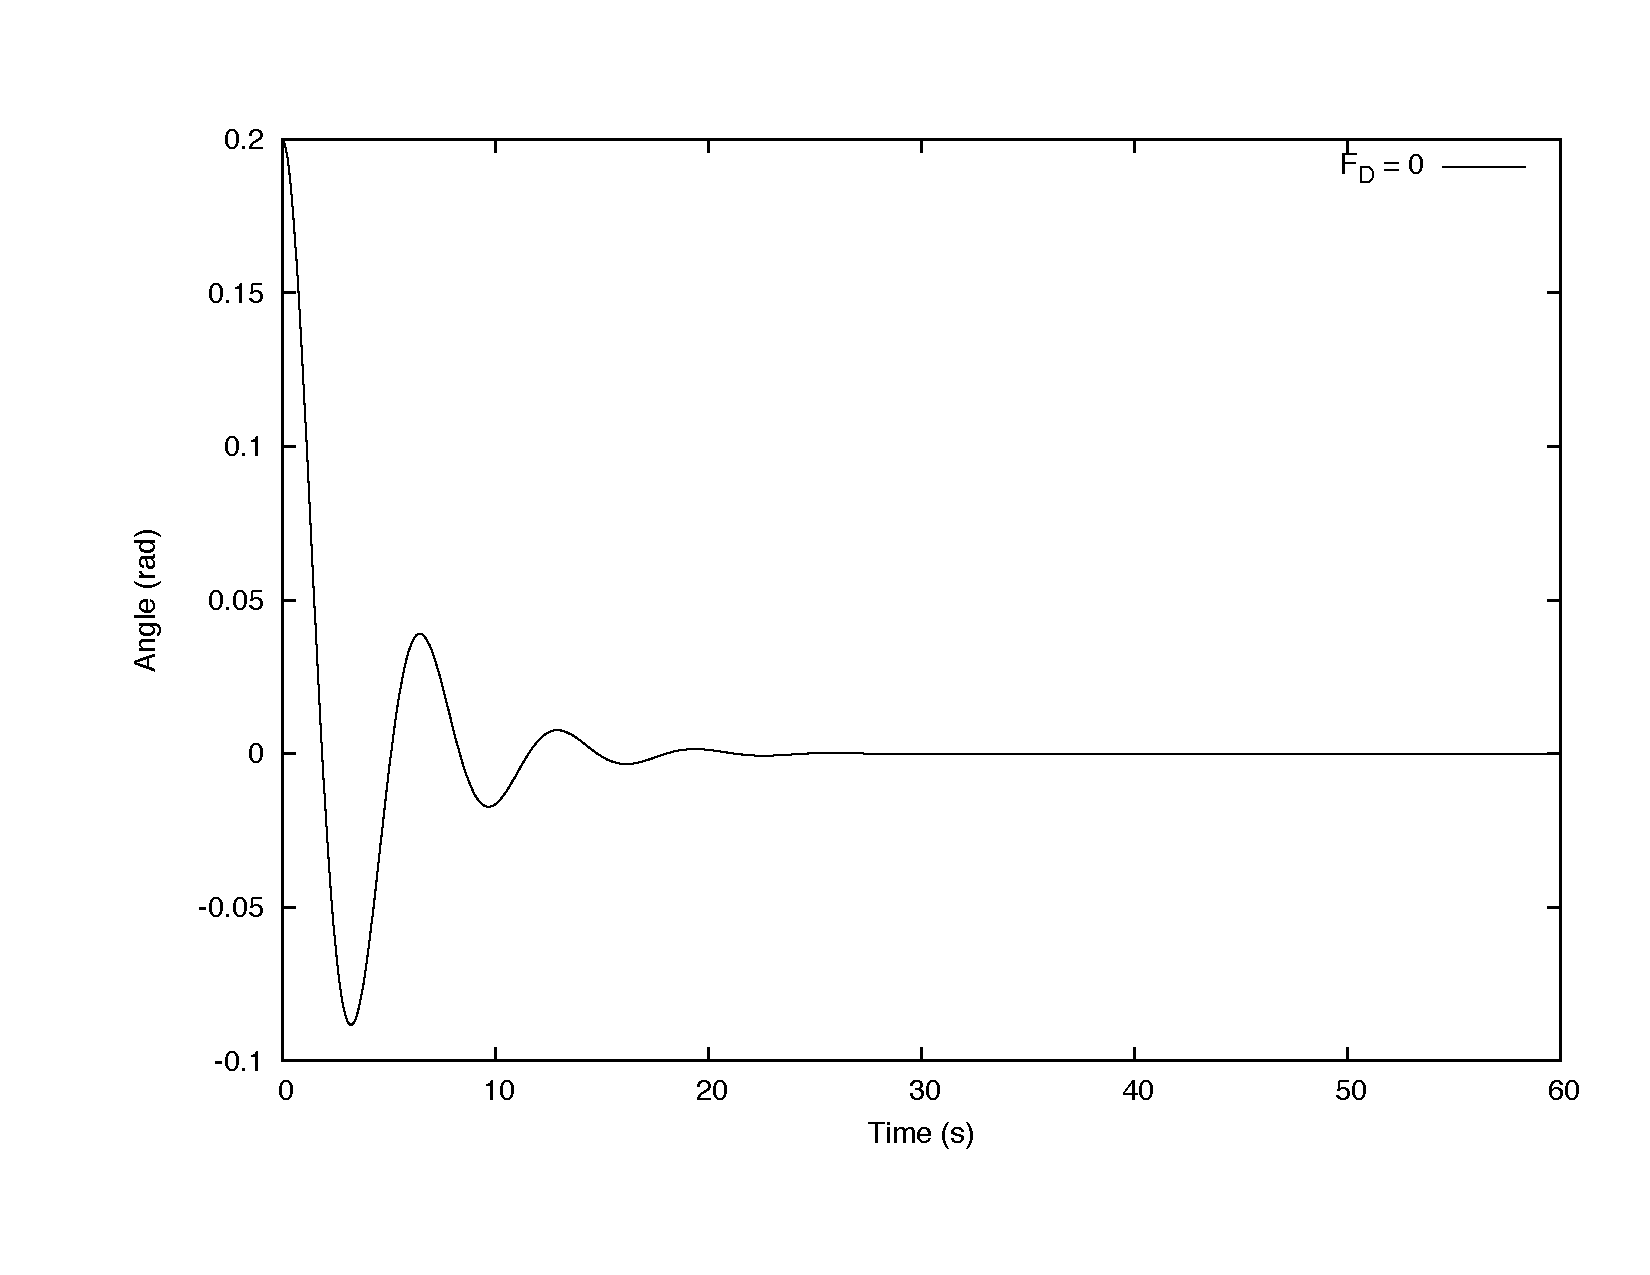
\includegraphics[width =120 mm, height = 75mm]{Fig_3_6_0_res.pdf}
\caption{Numeric solution to \eqref{SHMDampDriveNonLin} with $F_D=0$.}
\label{fig:3_6_0}
\end{figure}
\begin{figure}[!h]
\centering
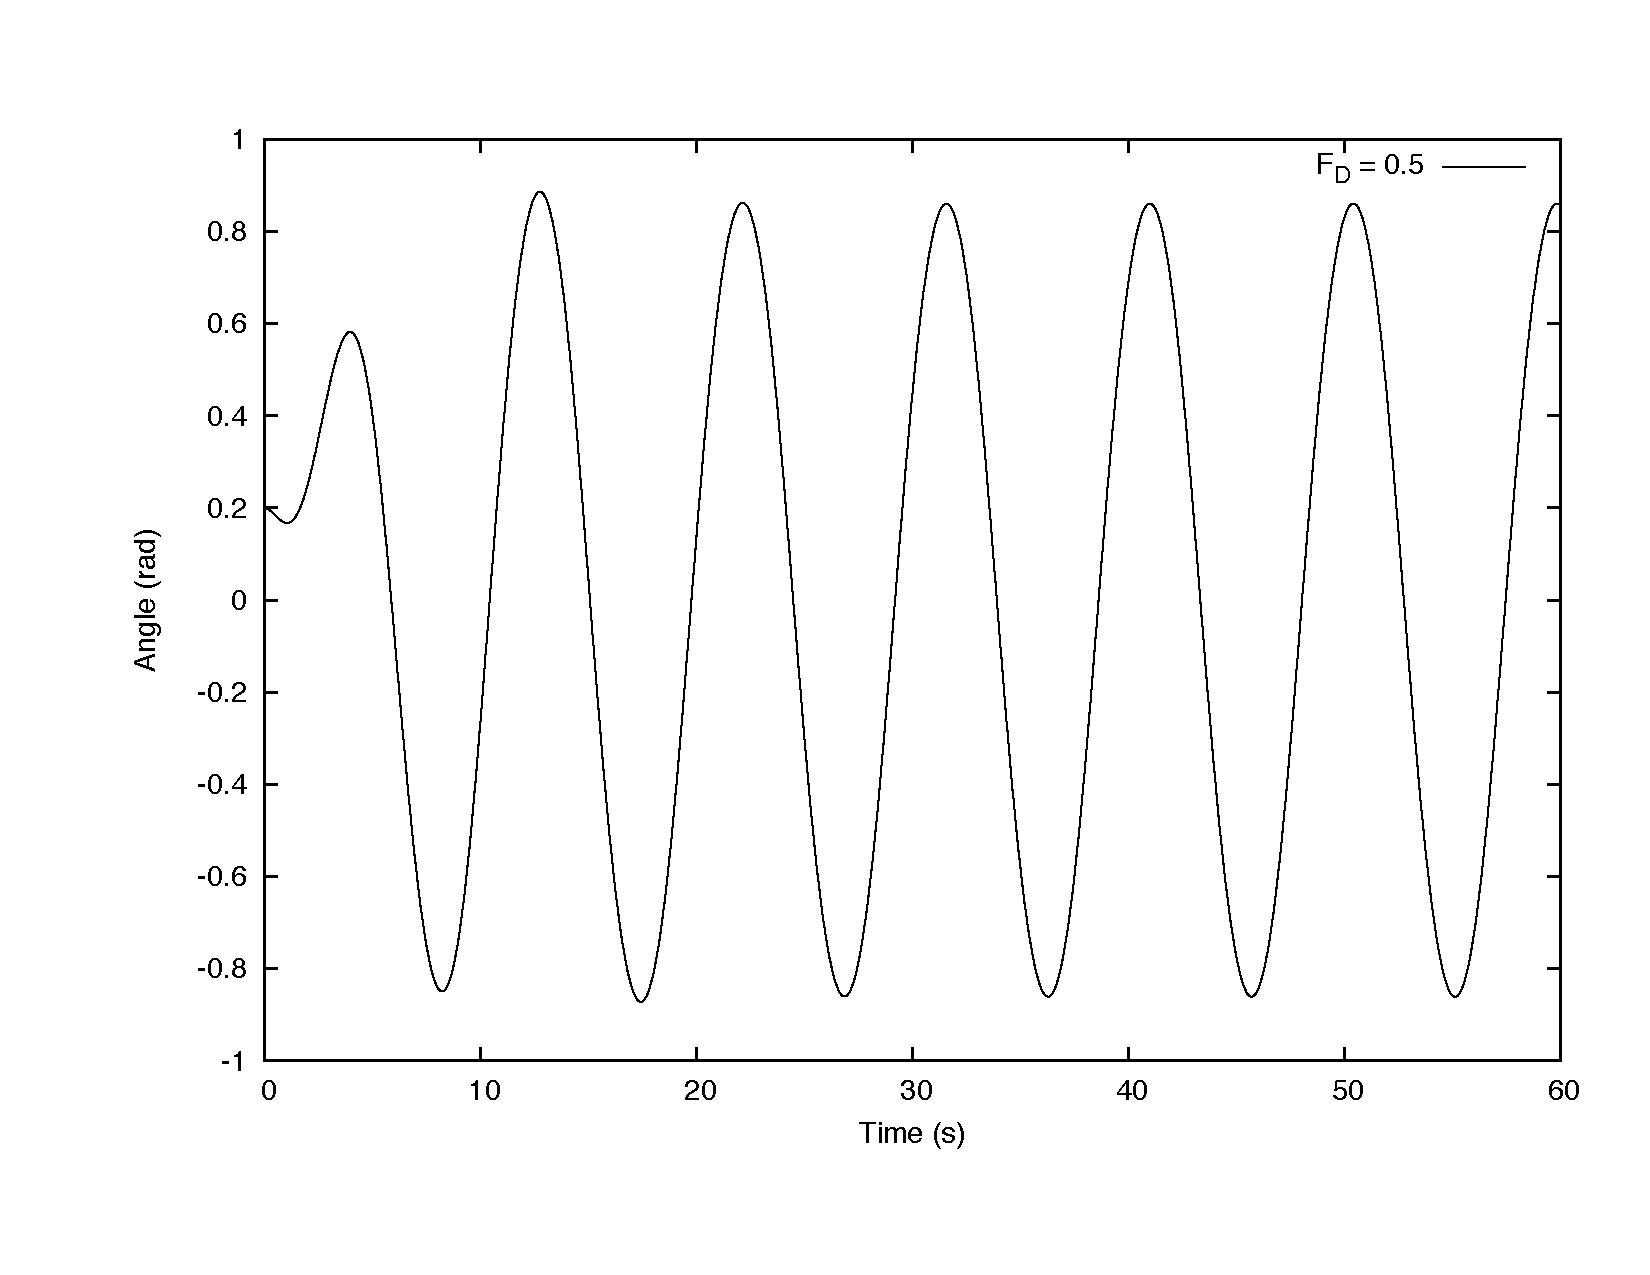
\includegraphics[width =110 mm, height = 59mm]{Fig_3_6_5_res.pdf}
\caption{Numeric solution to \eqref{SHMDampDriveNonLin} with $F_D=0.5$.}
\label{fig:3_6_5}
\end{figure}
\begin{figure}[!h]
\centering
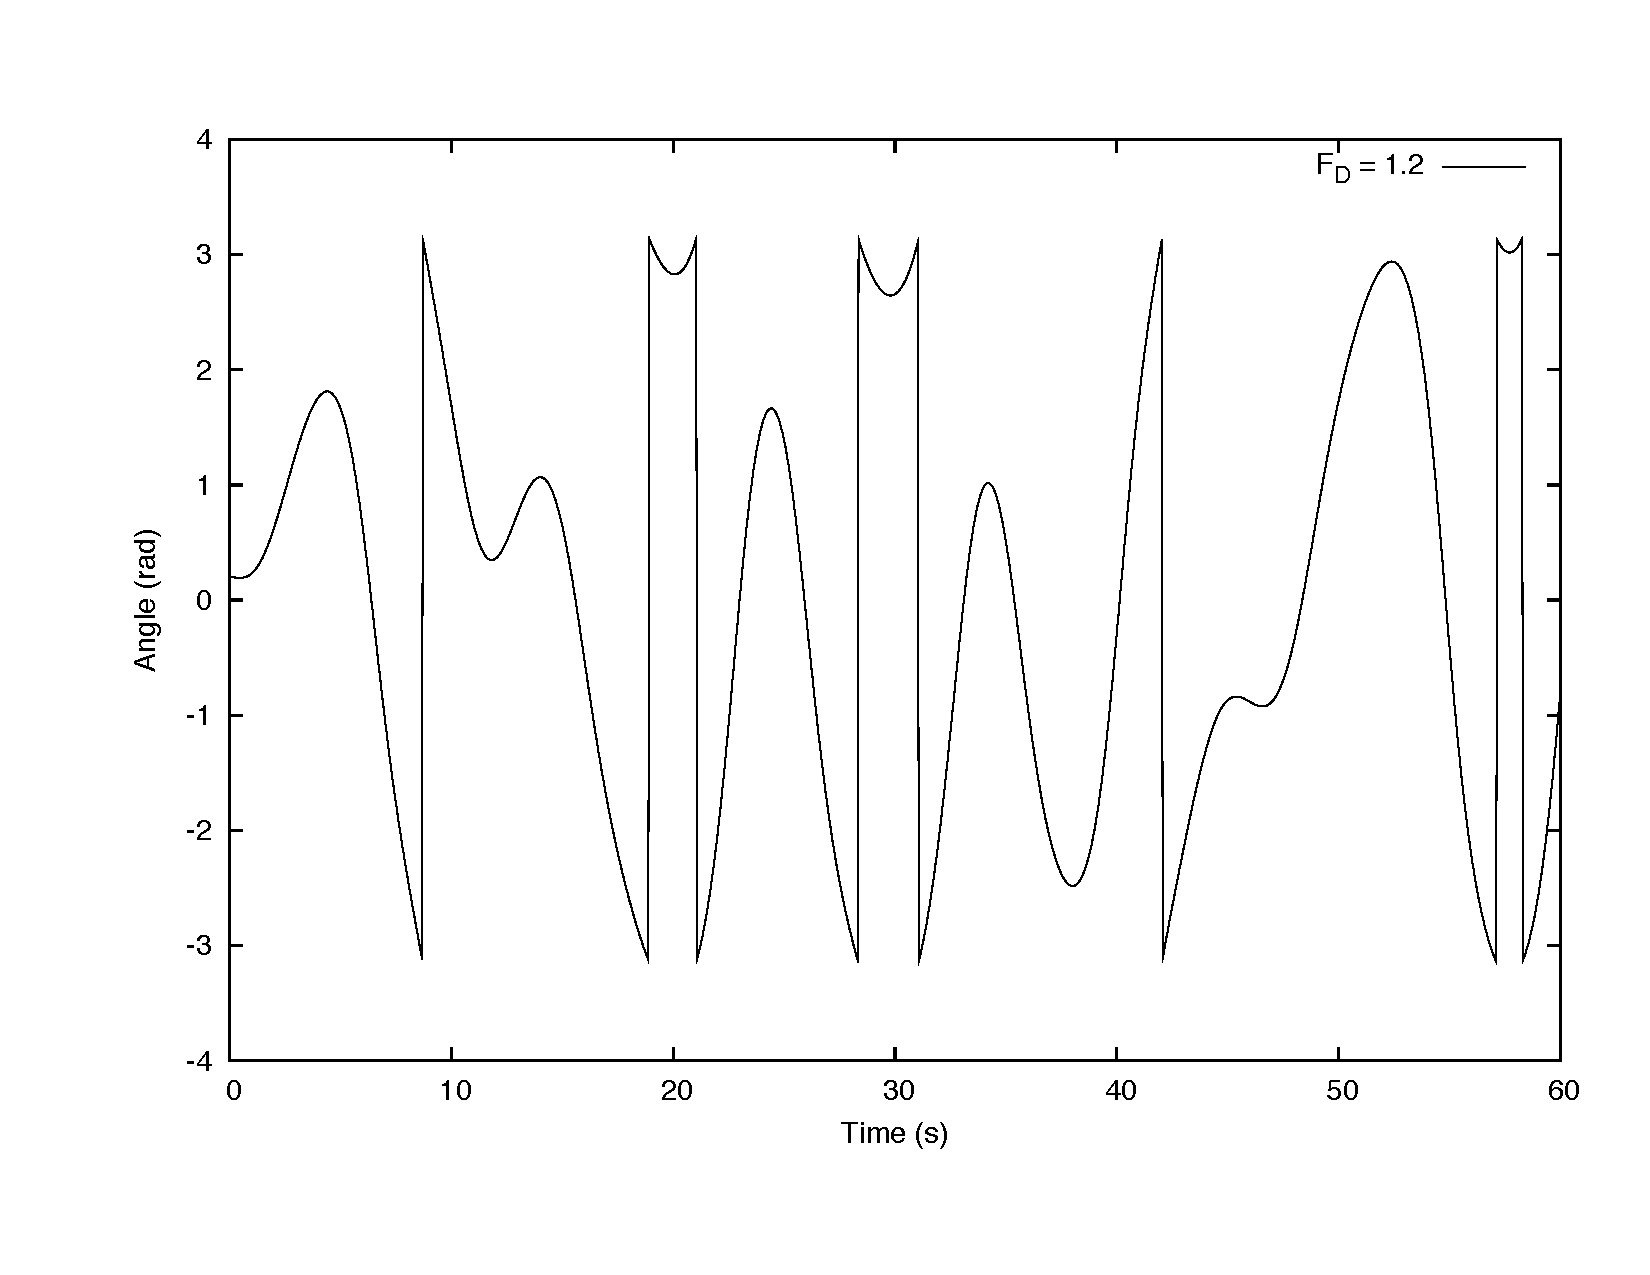
\includegraphics[width =110 mm, height = 59mm]{Fig_3_6_12_res.pdf}
\caption{Numeric solution to \eqref{SHMDampDriveNonLin} with $F_D=1.2$.  The discontinuities result from reseting any value of $|\theta|$ that is greater than $\pi$.}
\label{fig:3_6_12}
\end{figure}
\begin{figure}[!h]
\centering
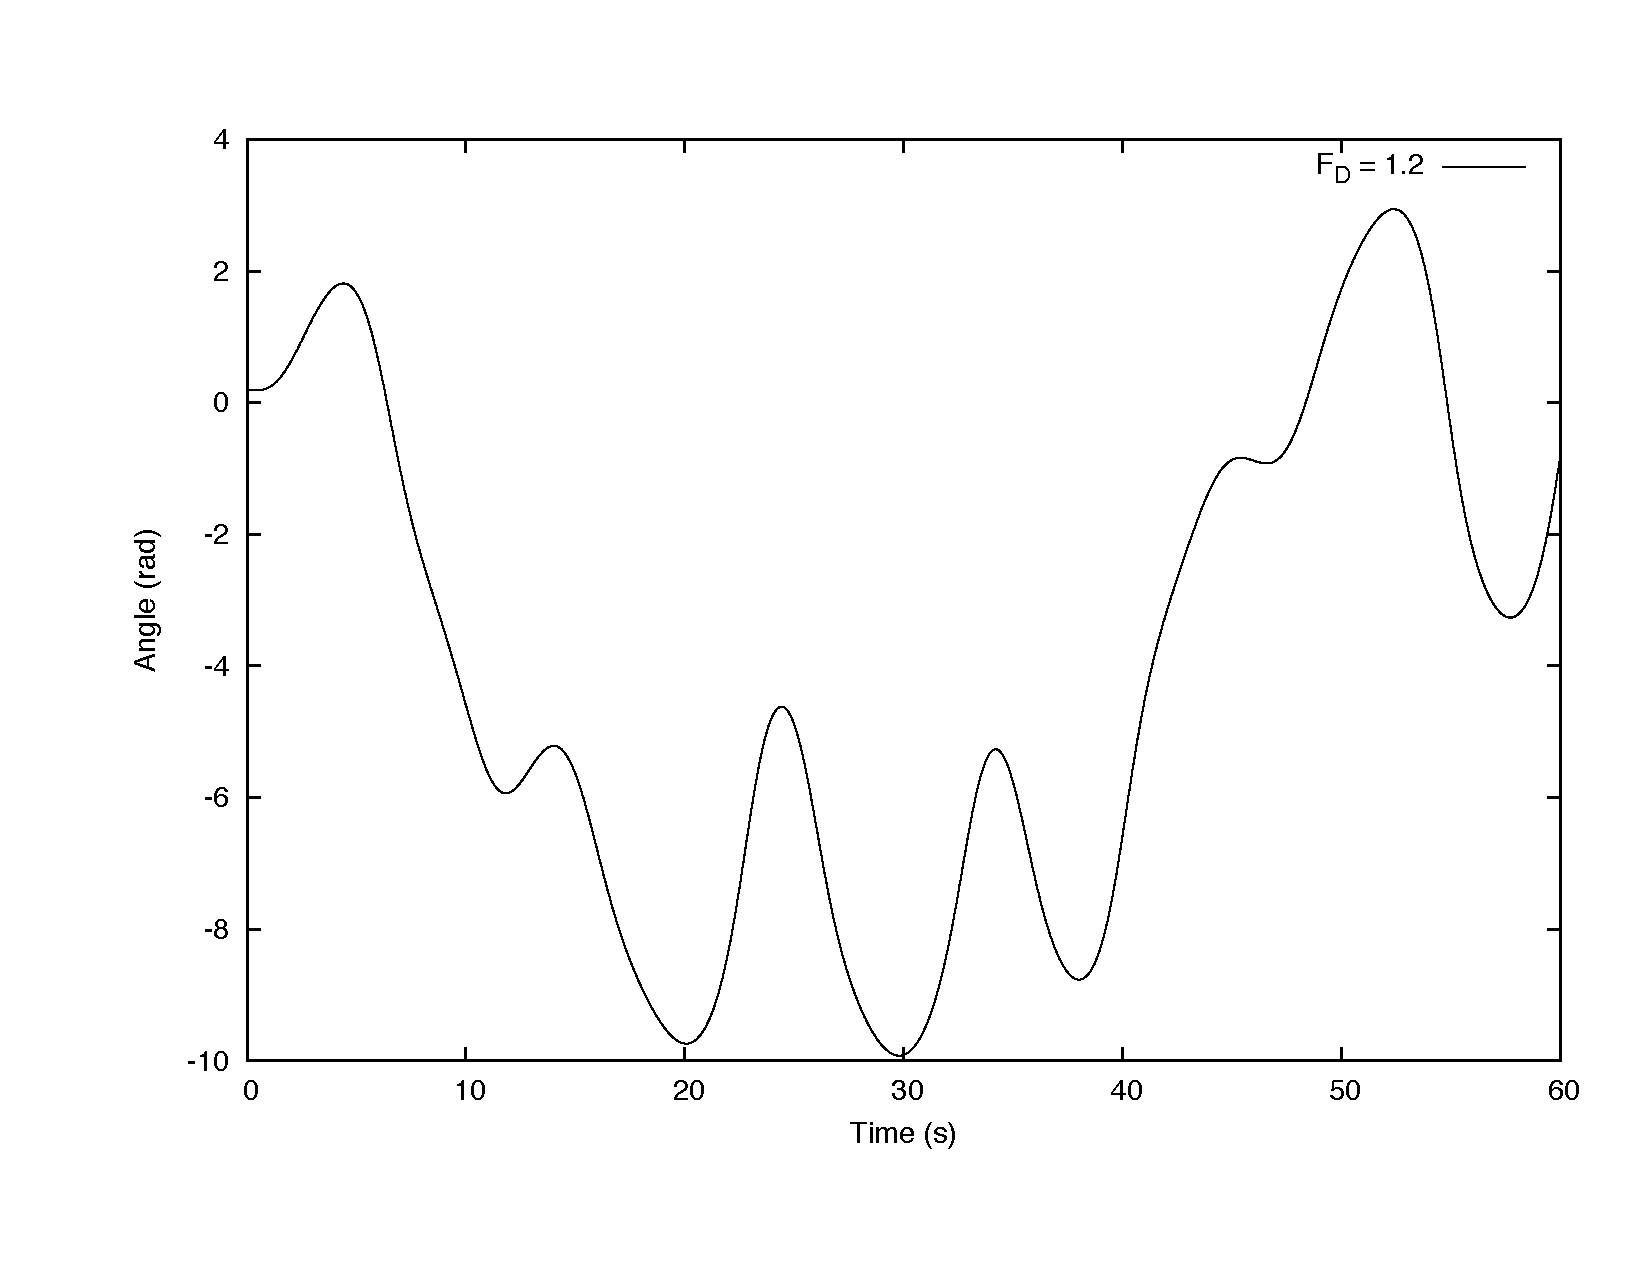
\includegraphics[width =110 mm, height = 59mm]{Fig_3_6_12_nores.pdf}
\caption{Numeric solution to \eqref{SHMDampDriveNonLin} with $F_D=1.2$.}
\label{fig:3_6_12_nores}
\end{figure}
\begin{figure}[!h]
\centering
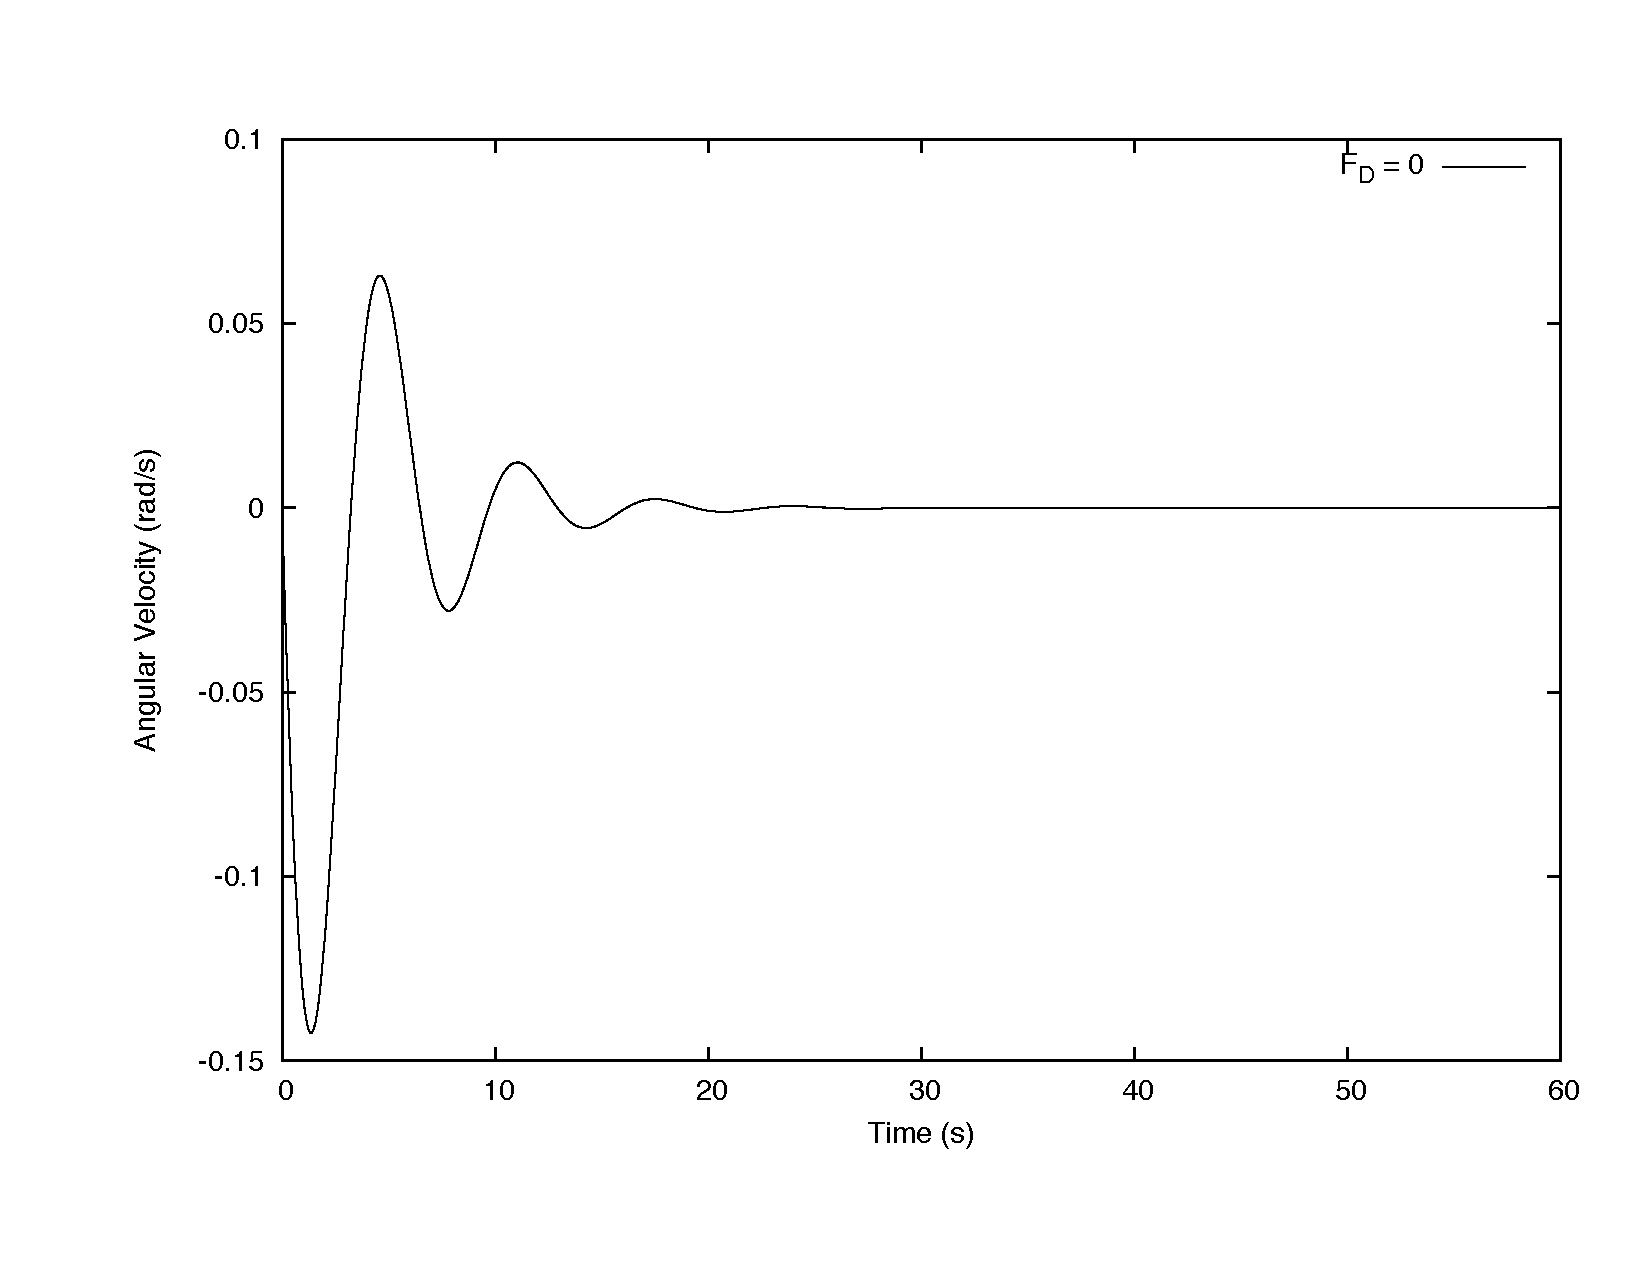
\includegraphics[width =110 mm, height = 59mm]{Fig_3_6_0_omeg.pdf}
\caption{Numeric solution to \eqref{SHMDampDriveNonLin} with $F_D=0.0$.}
\label{fig:3_6_0_omeg}
\end{figure}
\begin{figure}[!h]
\centering
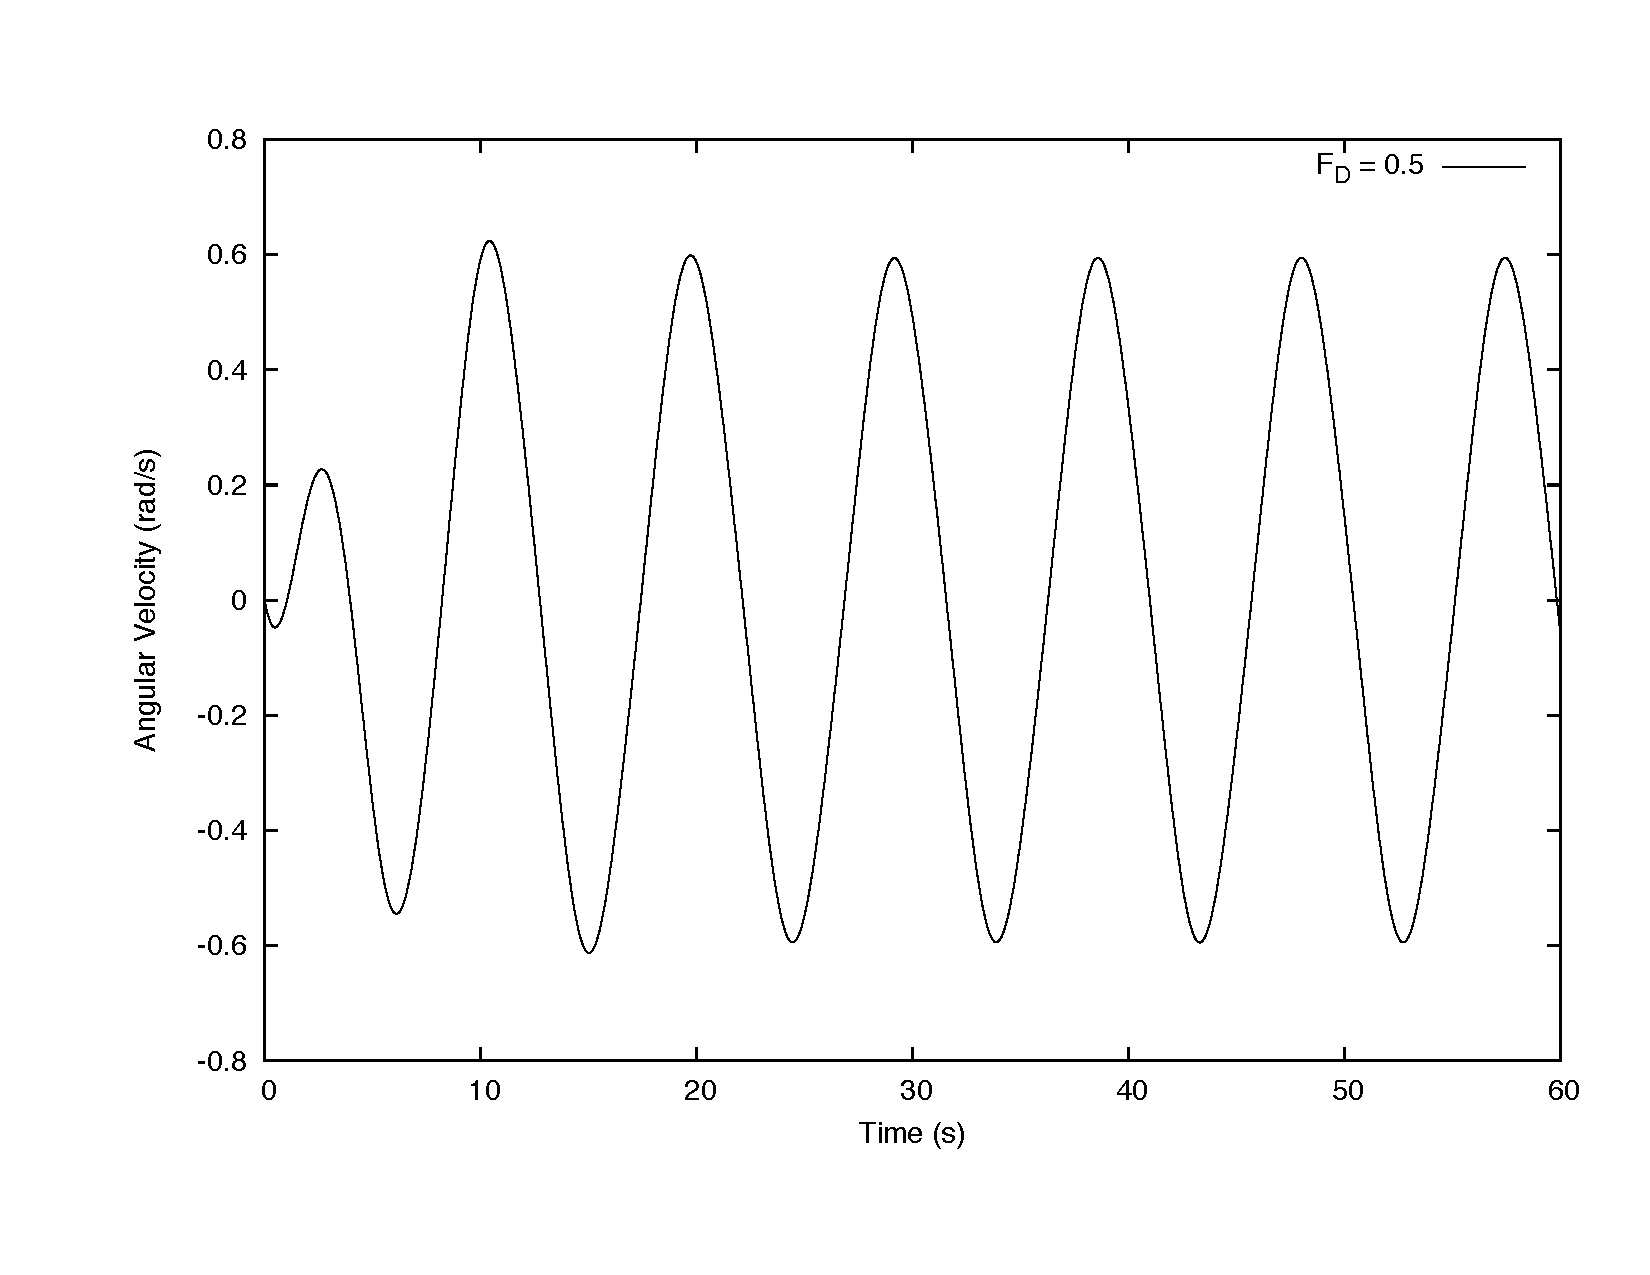
\includegraphics[width =110 mm, height = 59mm]{Fig_3_6_5_omeg.pdf}
\caption{Numeric solution to \eqref{SHMDampDriveNonLin} with $F_D=0.5$.}
\label{fig:3_6_5_omeg}
\end{figure}
\begin{figure}[!h]
\centering
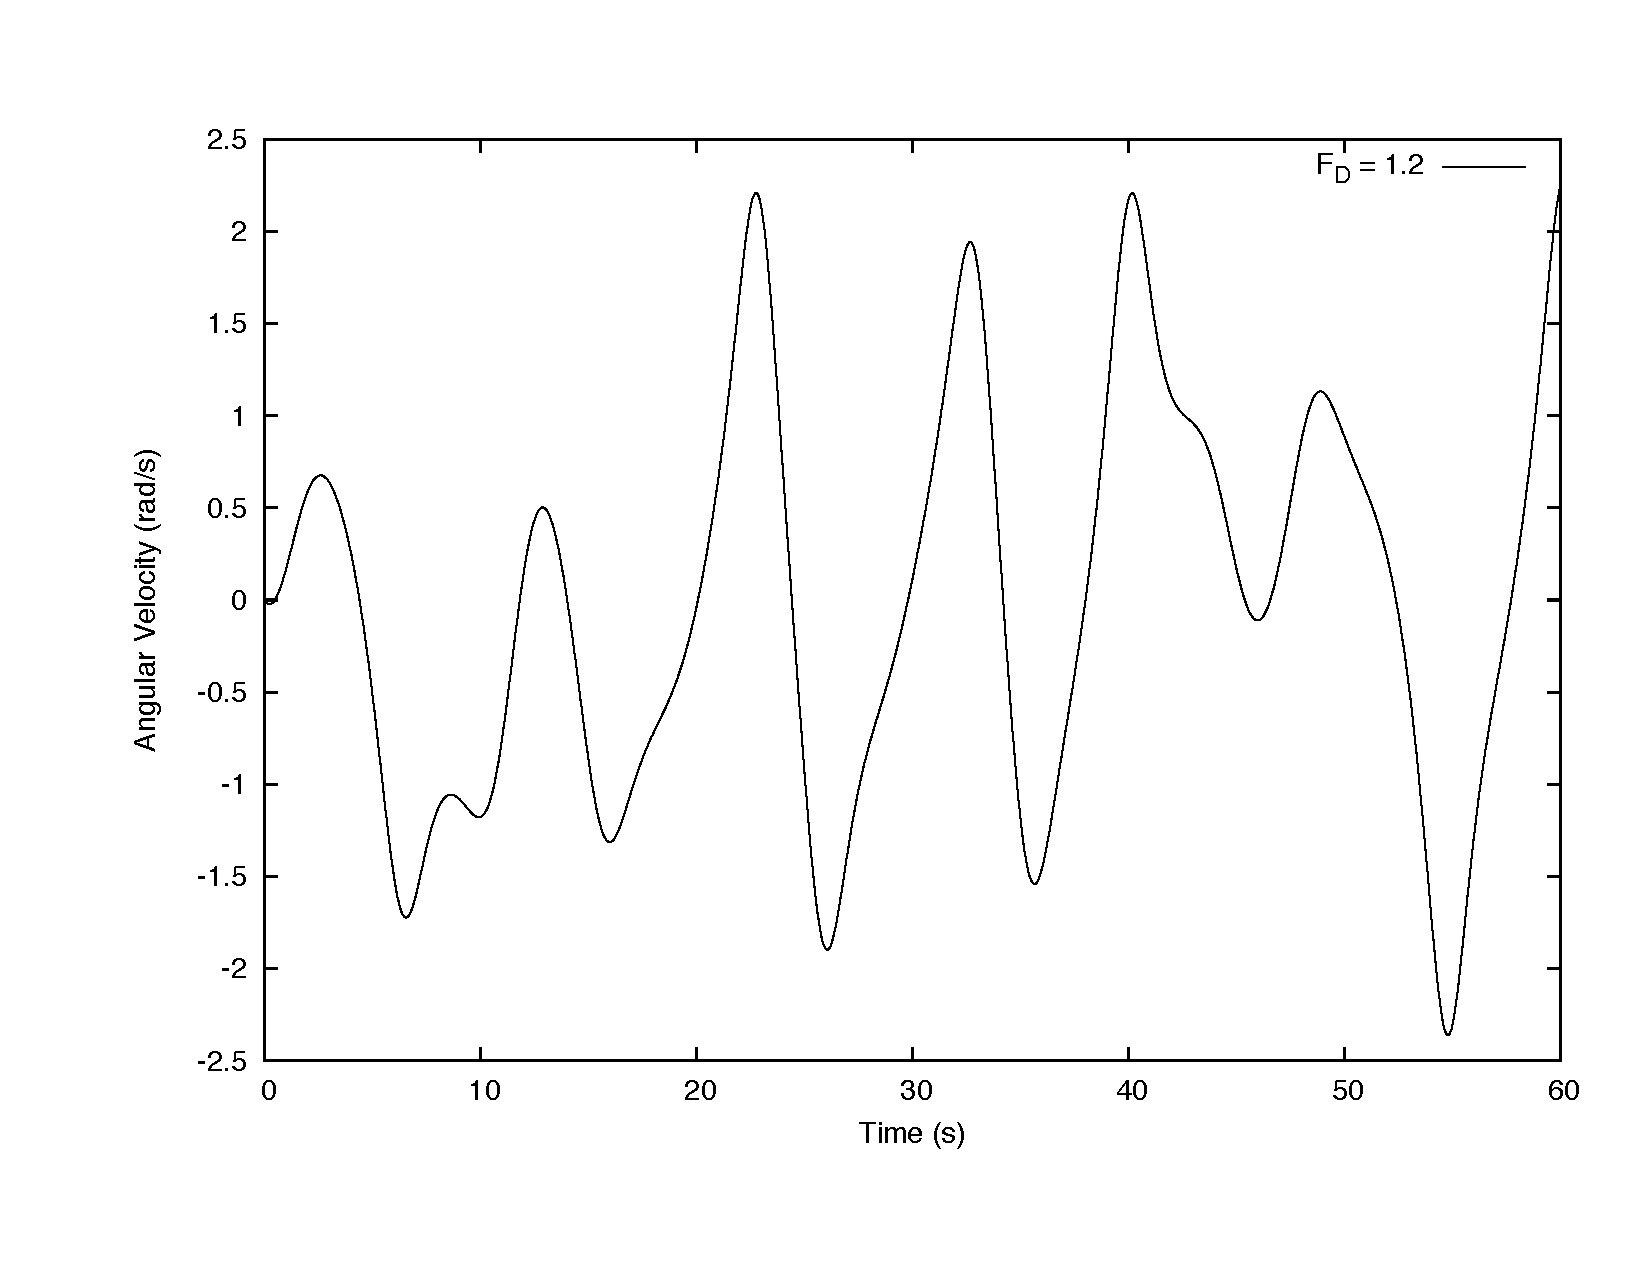
\includegraphics[width =110 mm, height = 59mm]{Fig_3_6_12_omeg.pdf}
\caption{Numeric solution to \eqref{SHMDampDriveNonLin} with $F_D=1.2$.}
\label{fig:3_6_12_omeg}
\end{figure}

Figures \ref{fig:3_6_0} through \ref{fig:3_6_12_nores} plot the angular position of the pendulum as a function of time at three different driving forces while figures \ref{fig:3_6_0_omeg} through \ref{fig:3_6_12_omeg} show the angular velocity as a function of time.  When there is no driving force ($F_D = 0$) one sees that the damping force causes the motion to decay away rapidly.  When the driving force is a small, non-zero value, one observes a simple oscillation that repeats for all time.  However, when the driving force becomes large, some very unique behavior is observed.  There seems to be no discernible pattern in the chaotic motion, however since the RK method was able to calculate it, there must be some pattern.  Further study of this problem results in the conclusion that the motion of this pendulum is both chaotic (thus unpredictable) and also deterministic.  

To understand this property, a phase space representation of the pendulum's motion is helpful.  A phase space diagram is a plot of the pendulum's angular position versus its angular velocity.  A specific type of phase space diagram, the Poincare section is a plot of these value at very precise intervals, namely when $\Omega_D t = 2n\pi$, or at time that are in phase with the driving force.
\begin{figure}[!h]
\centering
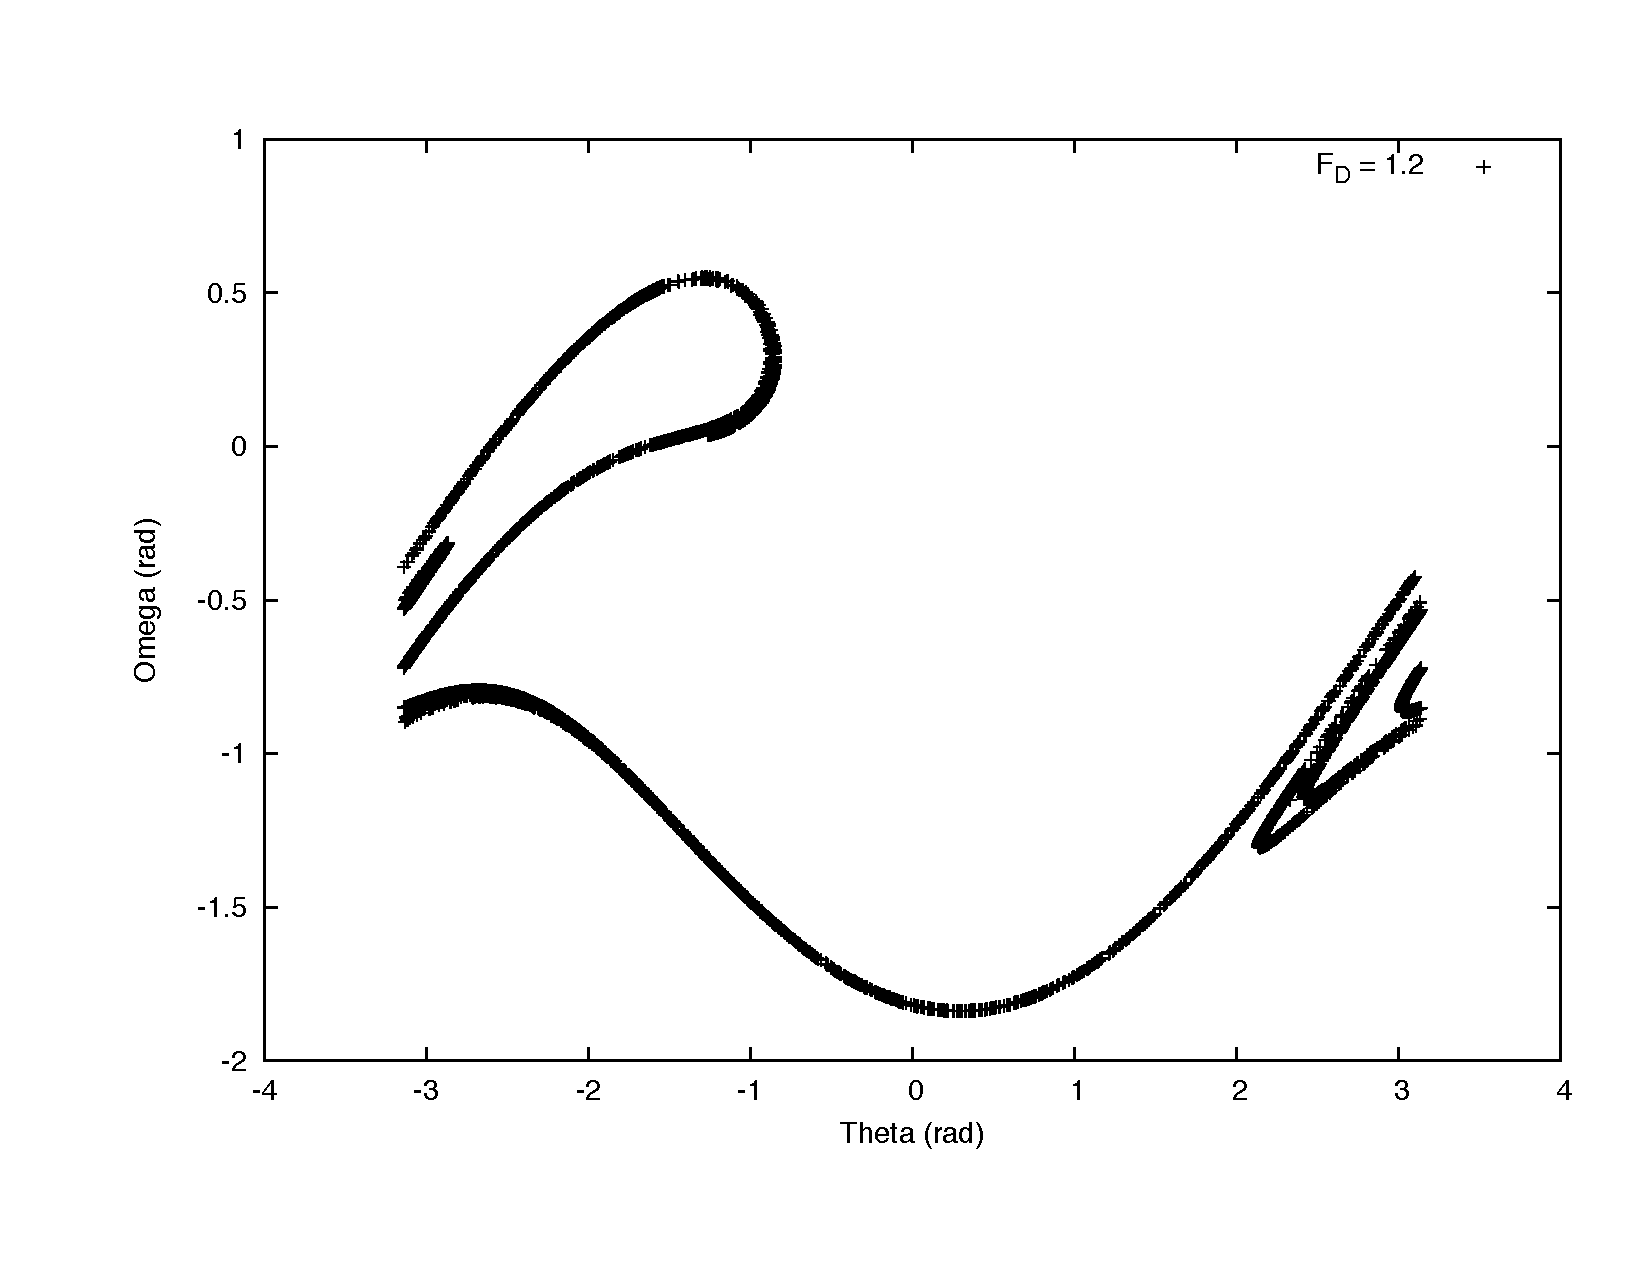
\includegraphics[width =120 mm, height = 80mm]{Fig_3_9.pdf}
\caption{A Poincare section of the damped driven pendulum with $F_D = 1.2$.}
\label{fig:3_9}
\end{figure}

The Poincare section of a chaotic system is the same, regardless of its initial conditions (if one disregards the initial, transient behavior).  The surface seen in Figure \ref{fig:3_9} is called a strange (due to the fuzzy nature) attractor.  Even though specific values of $\theta(t)$ cannot be predicted, the Poincare section provides values of $\omega$ and $\theta$ which match the surface of the attractor.

Now that the behavior in the chaotic regime has been explored, one may ask "when does the system become chaotic?"  
\begin{figure}[!h]
\centering
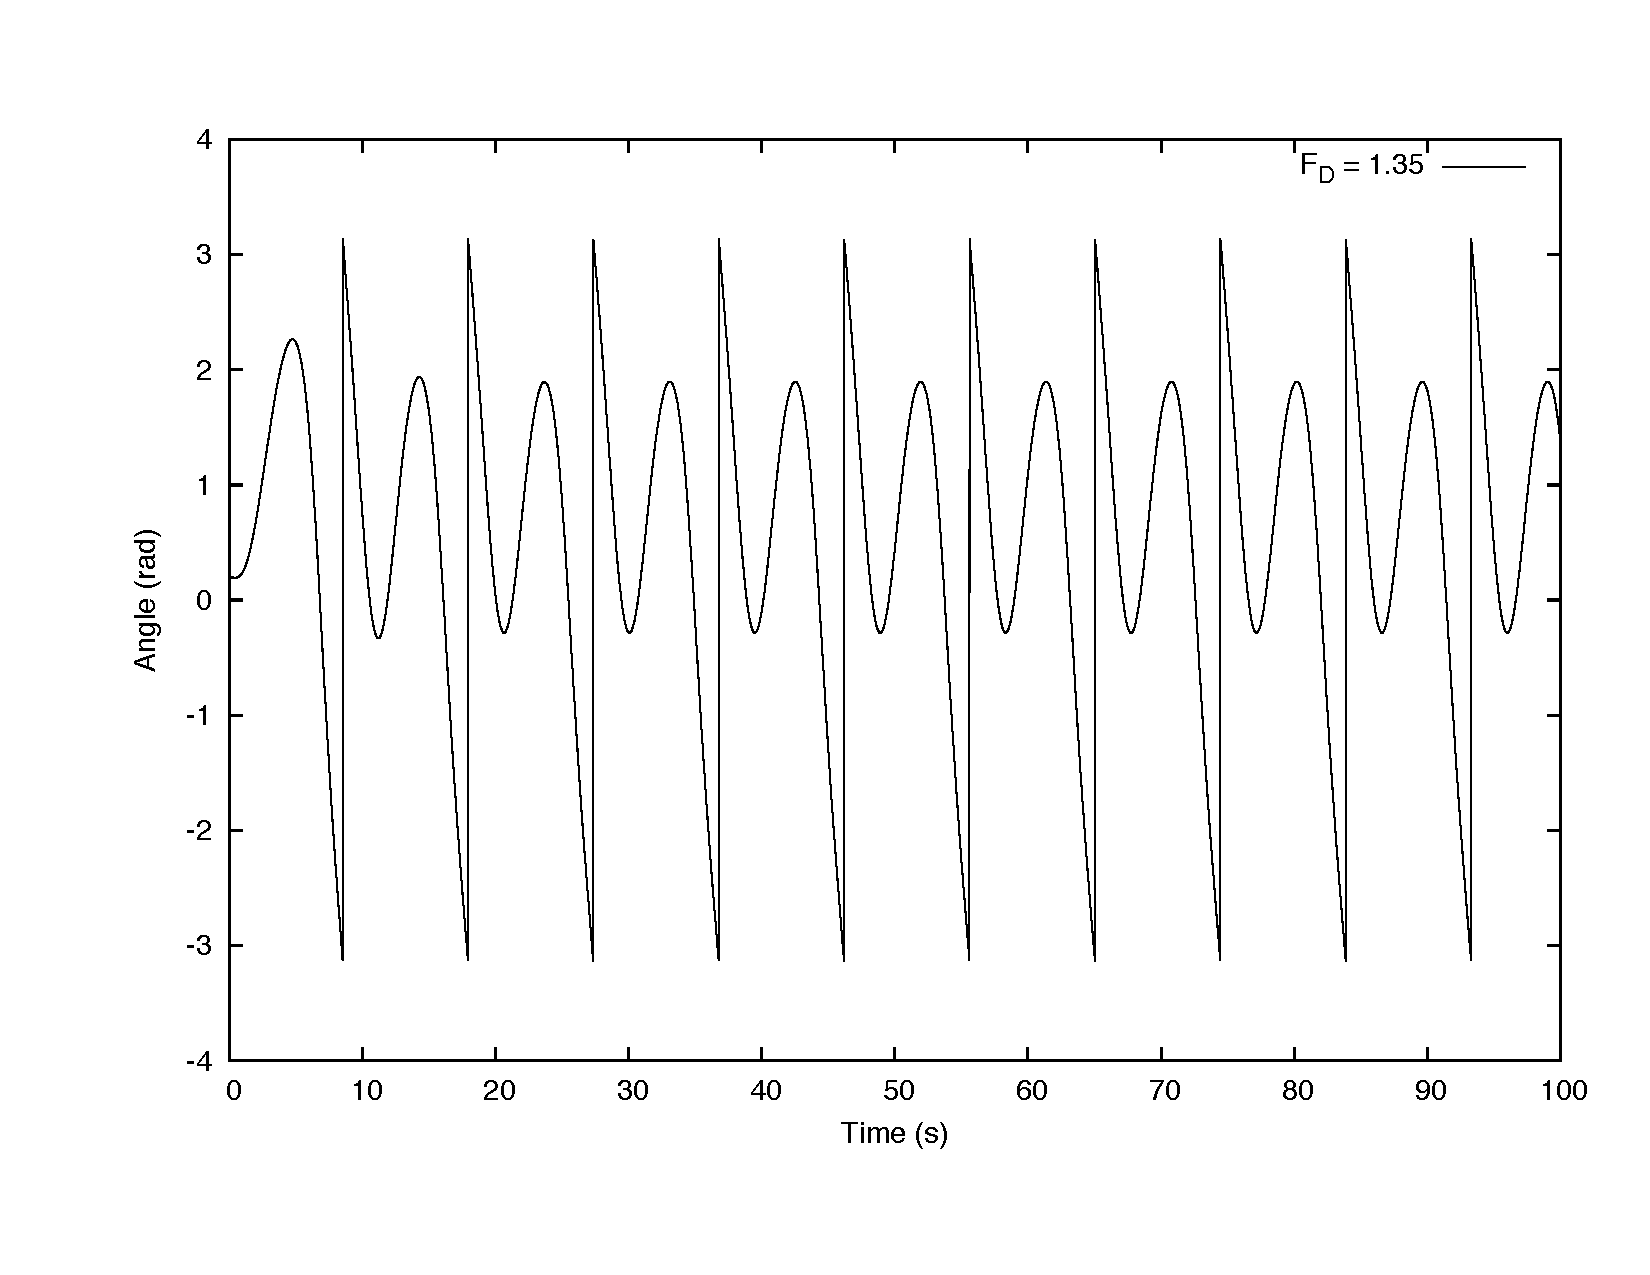
\includegraphics[width =110 mm, height = 80mm]{Fig_3_10_35.pdf}
\caption{Numeric solution to \eqref{SHMDampDriveNonLin} with $F_D=1.35$.}
\label{fig:3_10_35}
\end{figure}
\begin{figure}[!h]
\centering
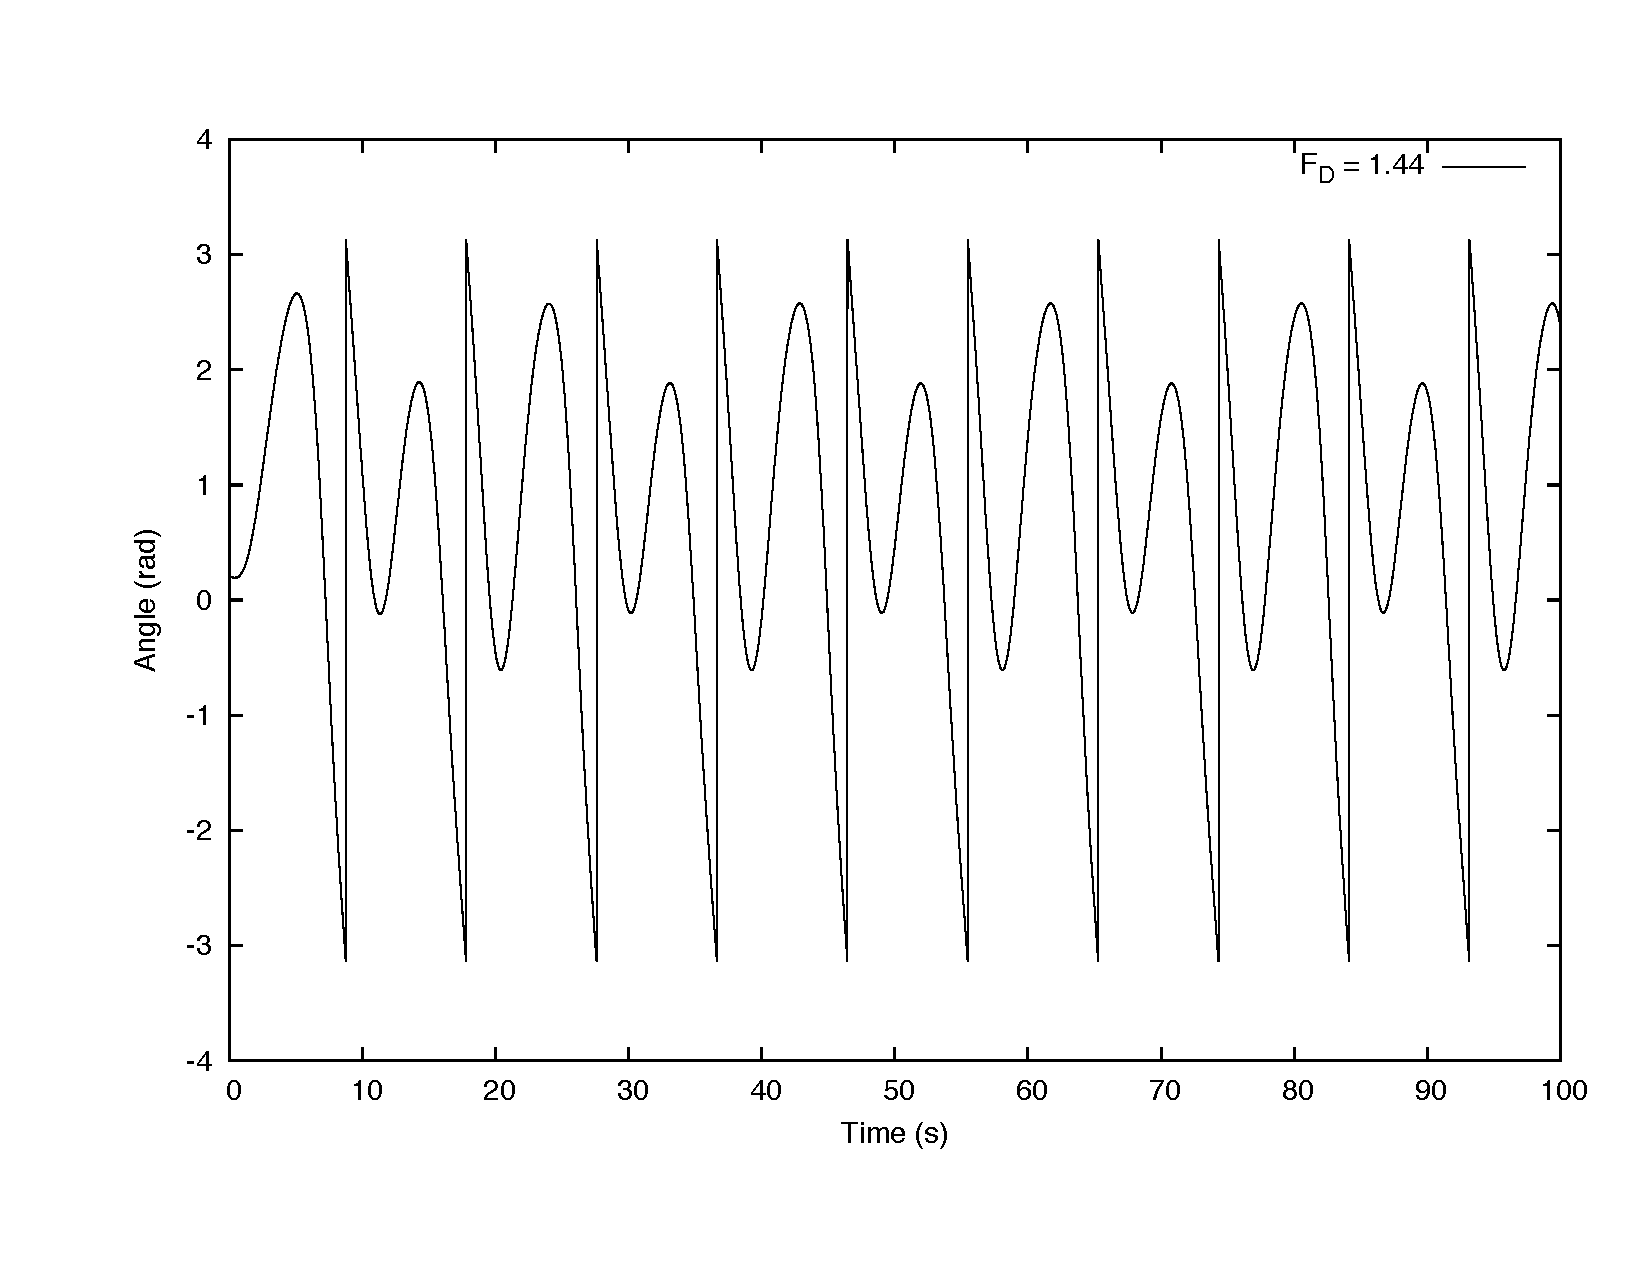
\includegraphics[width =110 mm, height = 65mm]{Fig_3_10_44.pdf}
\caption{Numeric solution to \eqref{SHMDampDriveNonLin} with $F_D=1.44$.}
\label{fig:3_10_44}
\end{figure}
\begin{figure}[!h]
\centering
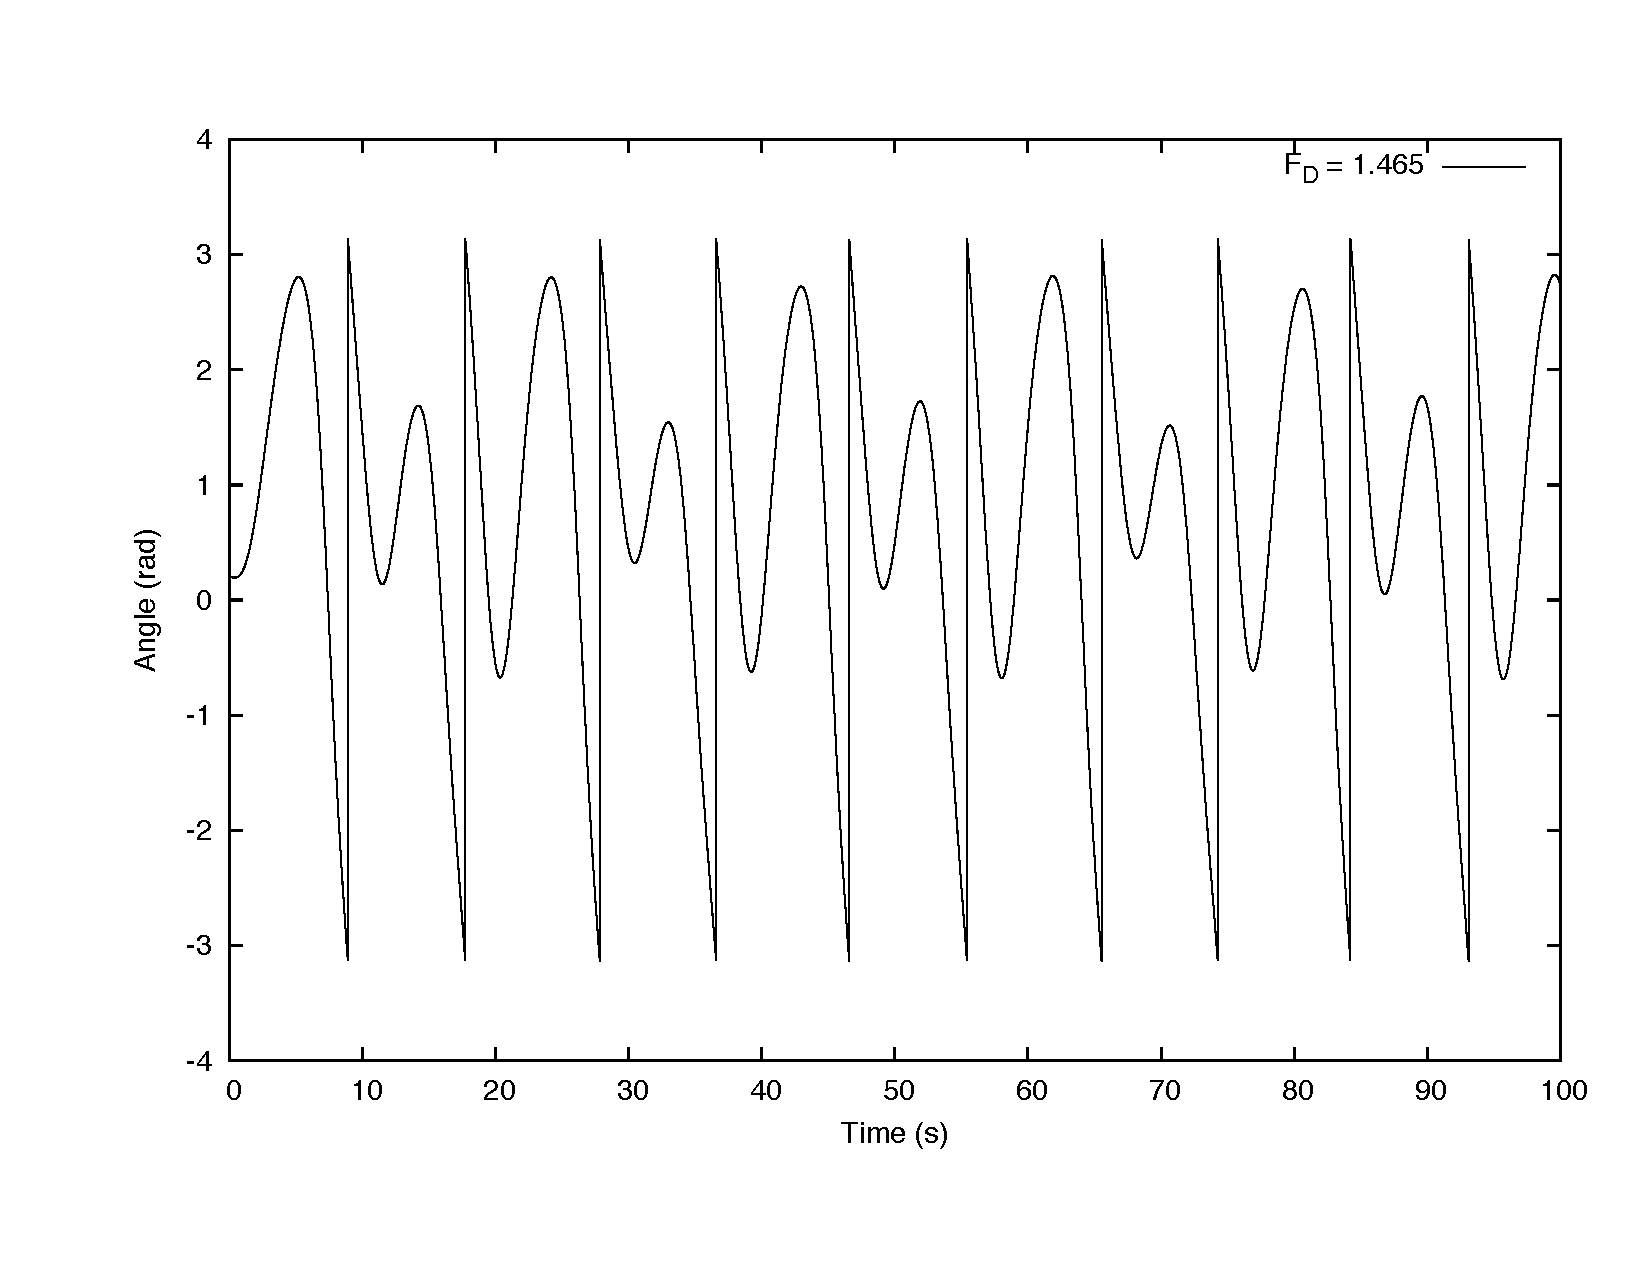
\includegraphics[width =110 mm, height = 65mm]{Fig_3_10_465.pdf}
\caption{Numeric solution to \eqref{SHMDampDriveNonLin} with $F_D=1.465$.}
\label{fig:3_10_465}
\end{figure}

Figures \ref{fig:3_10_35} through \ref{fig:3_10_465} show behavior called period doubling.  Although, on the surface, these three figures look very similar, if one pays close attention to the amplitude of the oscillations between angular resets, the unique properties become clear.  One sees the period doubling from the transition between Figure \ref{fig:3_10_35} and \ref{fig:3_10_44} and again from \ref{fig:3_10_44} to \ref{fig:3_10_465}.

To explore period doubling more thoroughly, a bifurcation diagram was constructed.  Bifurcation diagrams are plots of $\theta$ in phase with the driving force against the force amplitude, $F_D$.  At low values of $F_D$, there is only one value of $\theta$ that occurs in phase with the drive force.  However, as $F_D$ is increased, one observes two, then four, then many points that occur in phase with the driving frequency.  This cascade of period double is referred to as the 'path to chaos.'
\begin{figure}[!h]
\centering
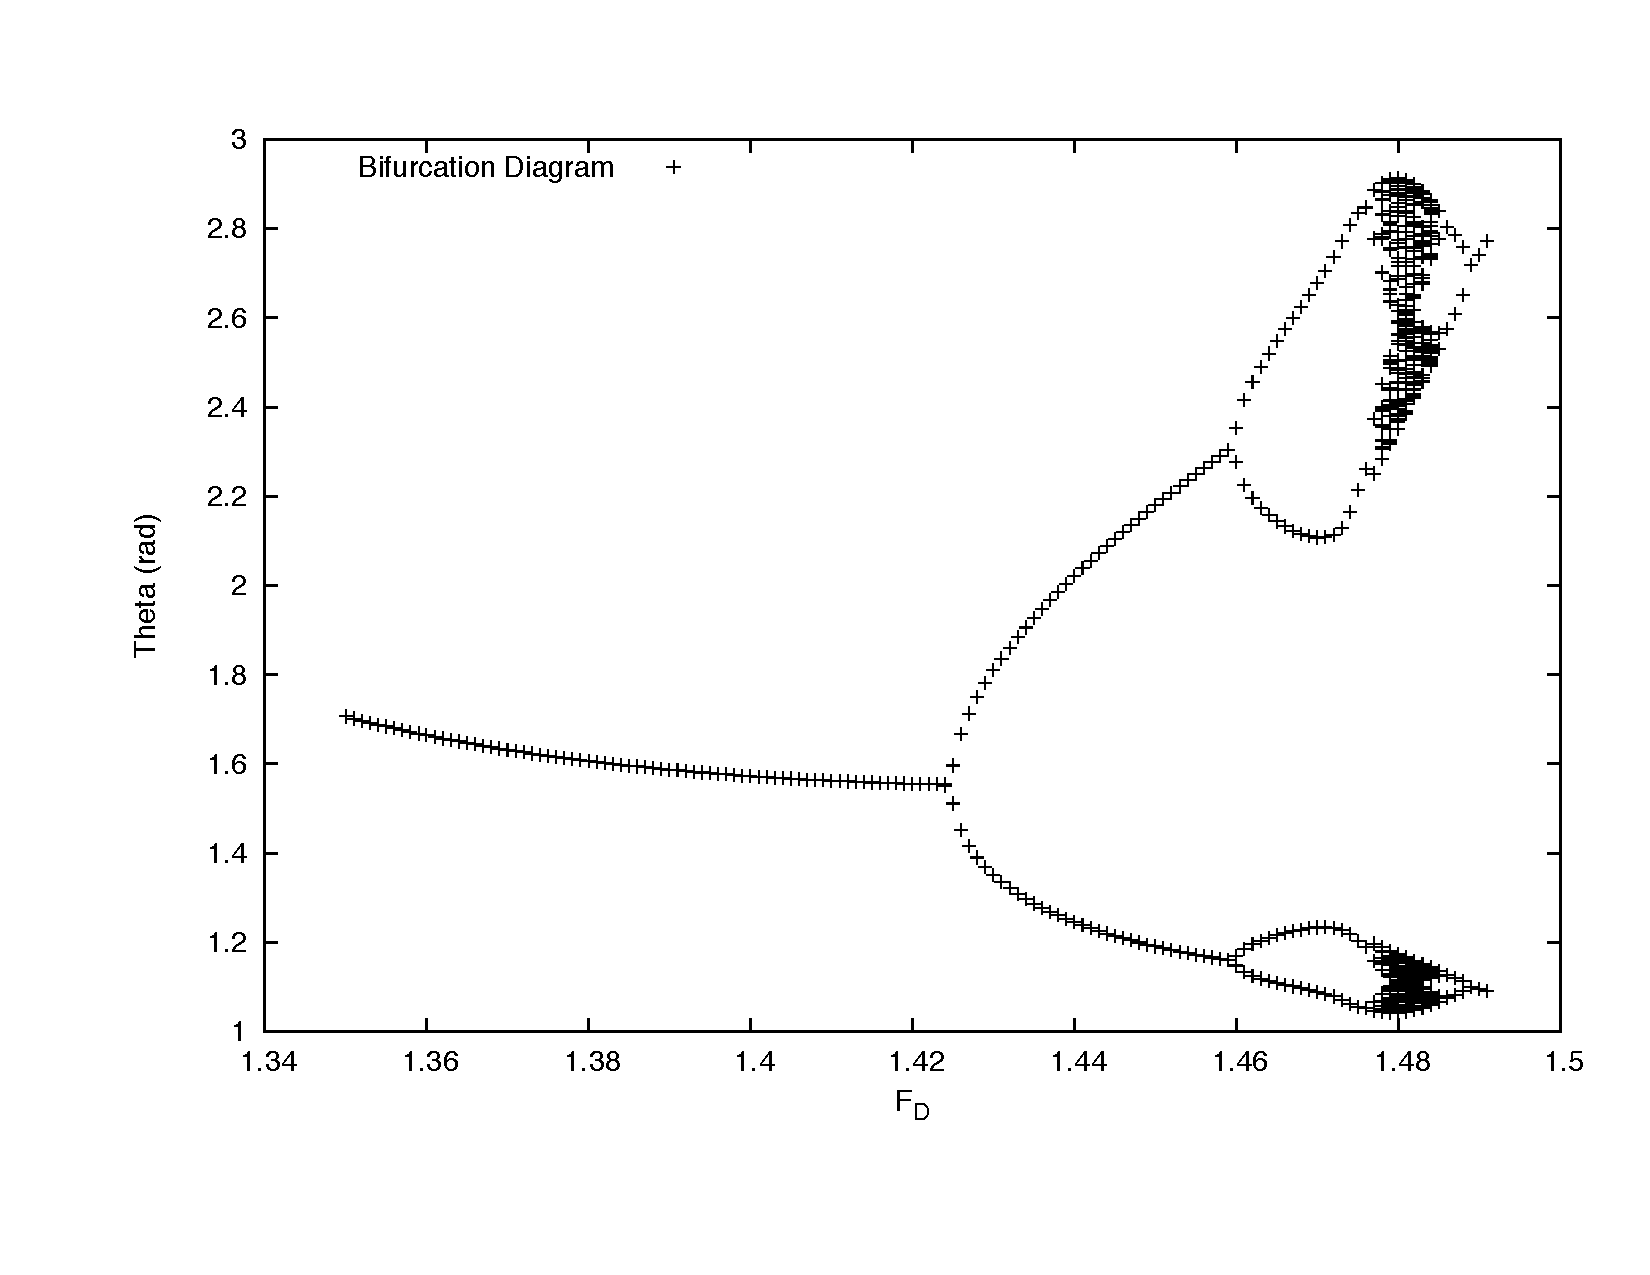
\includegraphics[width =110 mm, height = 65mm]{Fig_3_11.pdf}
\caption{Bifurcation diagram for the damped, driven pendulum.}
\label{fig:3_11}
\end{figure}

\subsection{Duffing Oscillator}
The next application of the RK methods the Duffing Oscillator.  The Duffing oscillator is another periodic potential well that causes chaotic behavior.  
\begin{equation}
\label{duff}
\ddot{x} = -c\dot{x}+bx-dx^3+F\cos{(\omega t)} 
\end{equation}
\eqref{duff} describes a pair of potential wells brought together to form two wells connected by a small, quadratic barrier.
\begin{equation}
\label{duffV}
V(x)=-\frac{1}{2}x^2+\frac{1}{4}x^4
\end{equation}
For the approximations performed in this lab, the following parameters were used:  $c=0.24, F=0.68, \omega = 1.7, b=d=1$ and initial conditions $x(0) = 1$ and $\dot{x}(0)=-1$.  Similar chaotic behavior as discussed above can be observed in the Duffing oscillator.  To explore these properties, another Poincare section was developed.
\begin{figure}[!h]
\centering
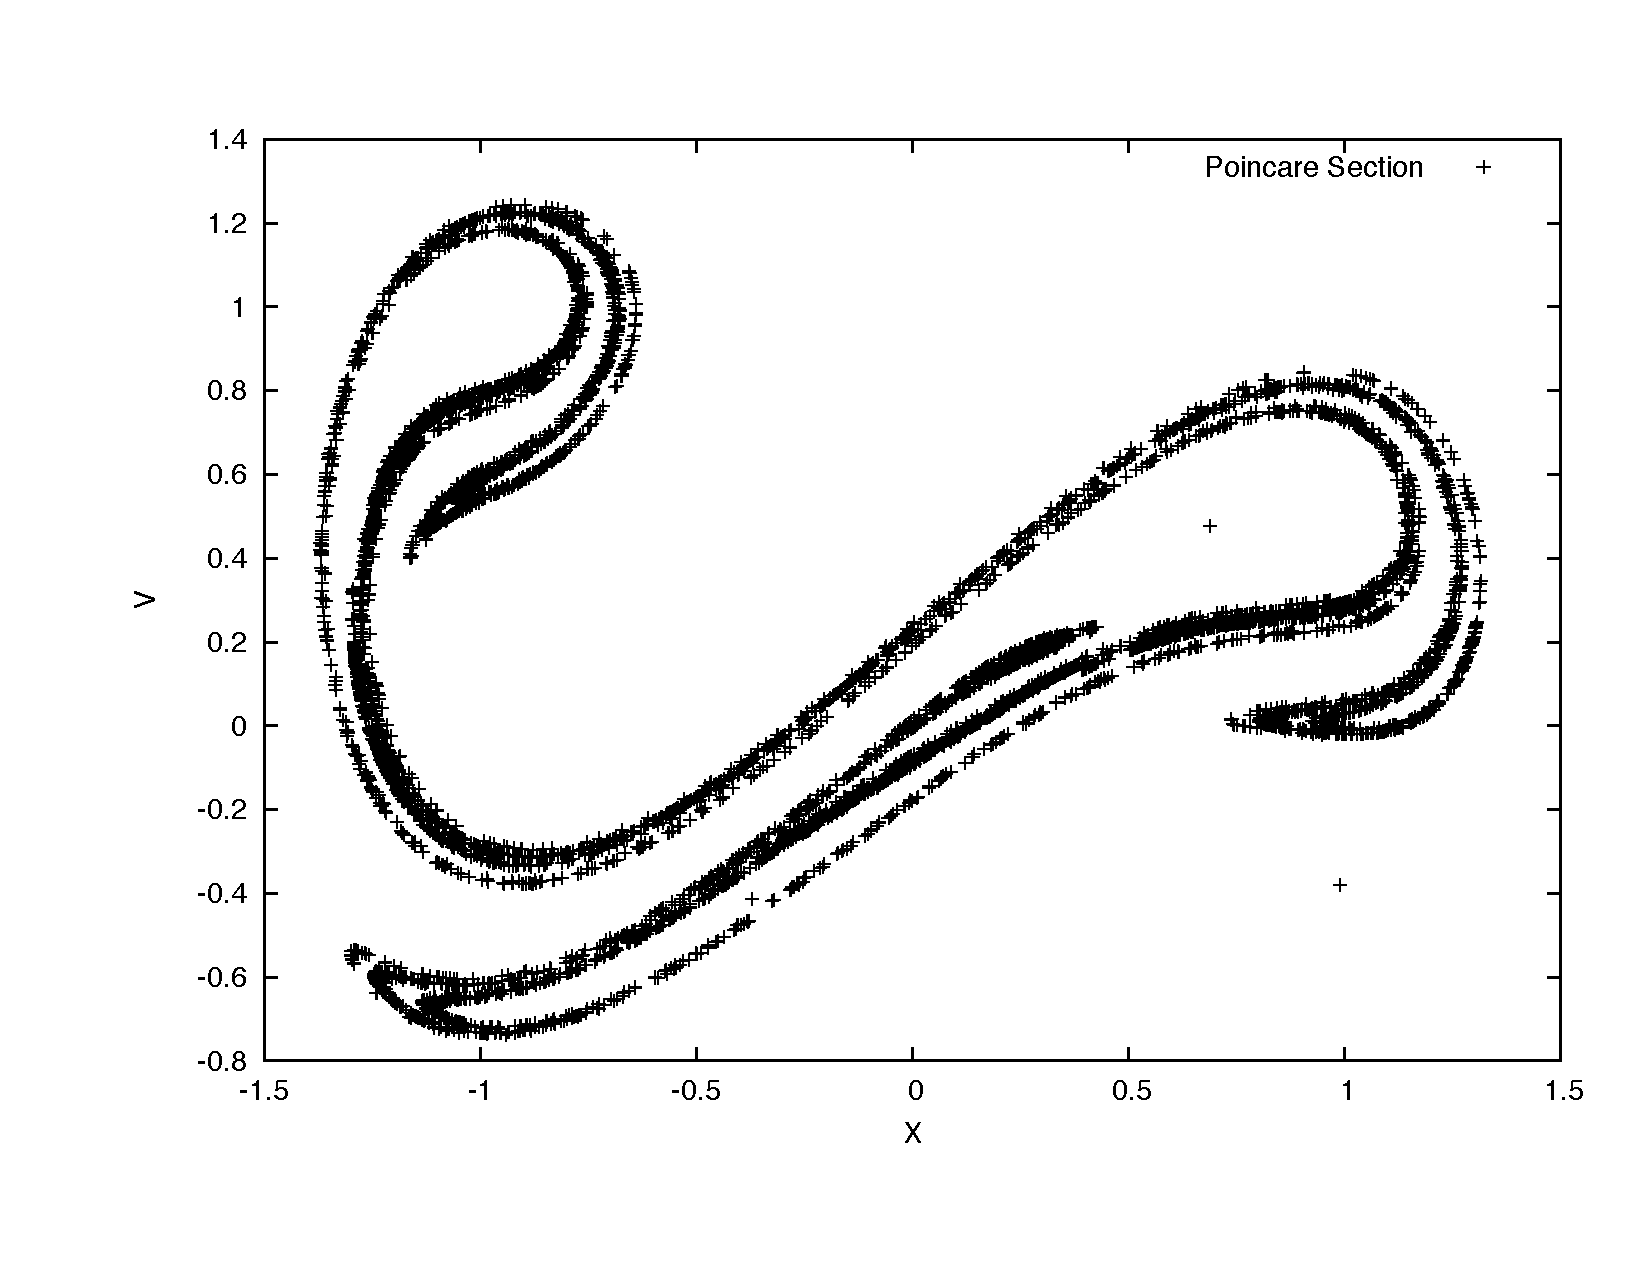
\includegraphics[width =110 mm, height = 60mm]{Fig_12_12.pdf}
\caption{Poincare section of the Duffing oscillator.}
\label{fig:12_12}
\end{figure}

Once again, there is a clearly defined surface that the system attracts to after the initial, transient oscillations have decayed away.  Another interesting feature of the Poincare section is its fractal nature.  Although none of the sections developed in this report had enough points to demonstrate this behavior, if one were to zoom in closely on a highly detailed Poincare section, one would observe similar patterns at all levels of zoom.
\subsection{Van der Pol Oscillator}
The final oscillator application of the RK method is the Van der Pol oscillator.  The Van der Pol oscillator equation was developed describe the behavior of an electrical circuit using triodes.
\begin{equation}
\label{van}
\ddot{x} = -x-\epsilon(x^2-1)\dot{x}
\end{equation}
For the sake of simplicity, $\epsilon=1$, and the initial conditions were defined as $x(0)=0.5$ and $\dot{x}(0)=0$.   Several plots were generated to show the behavior of this system, shown in \ref{fig:5_10a} through \ref{fig:5_10d}.
\begin{figure}[!h]
\centering
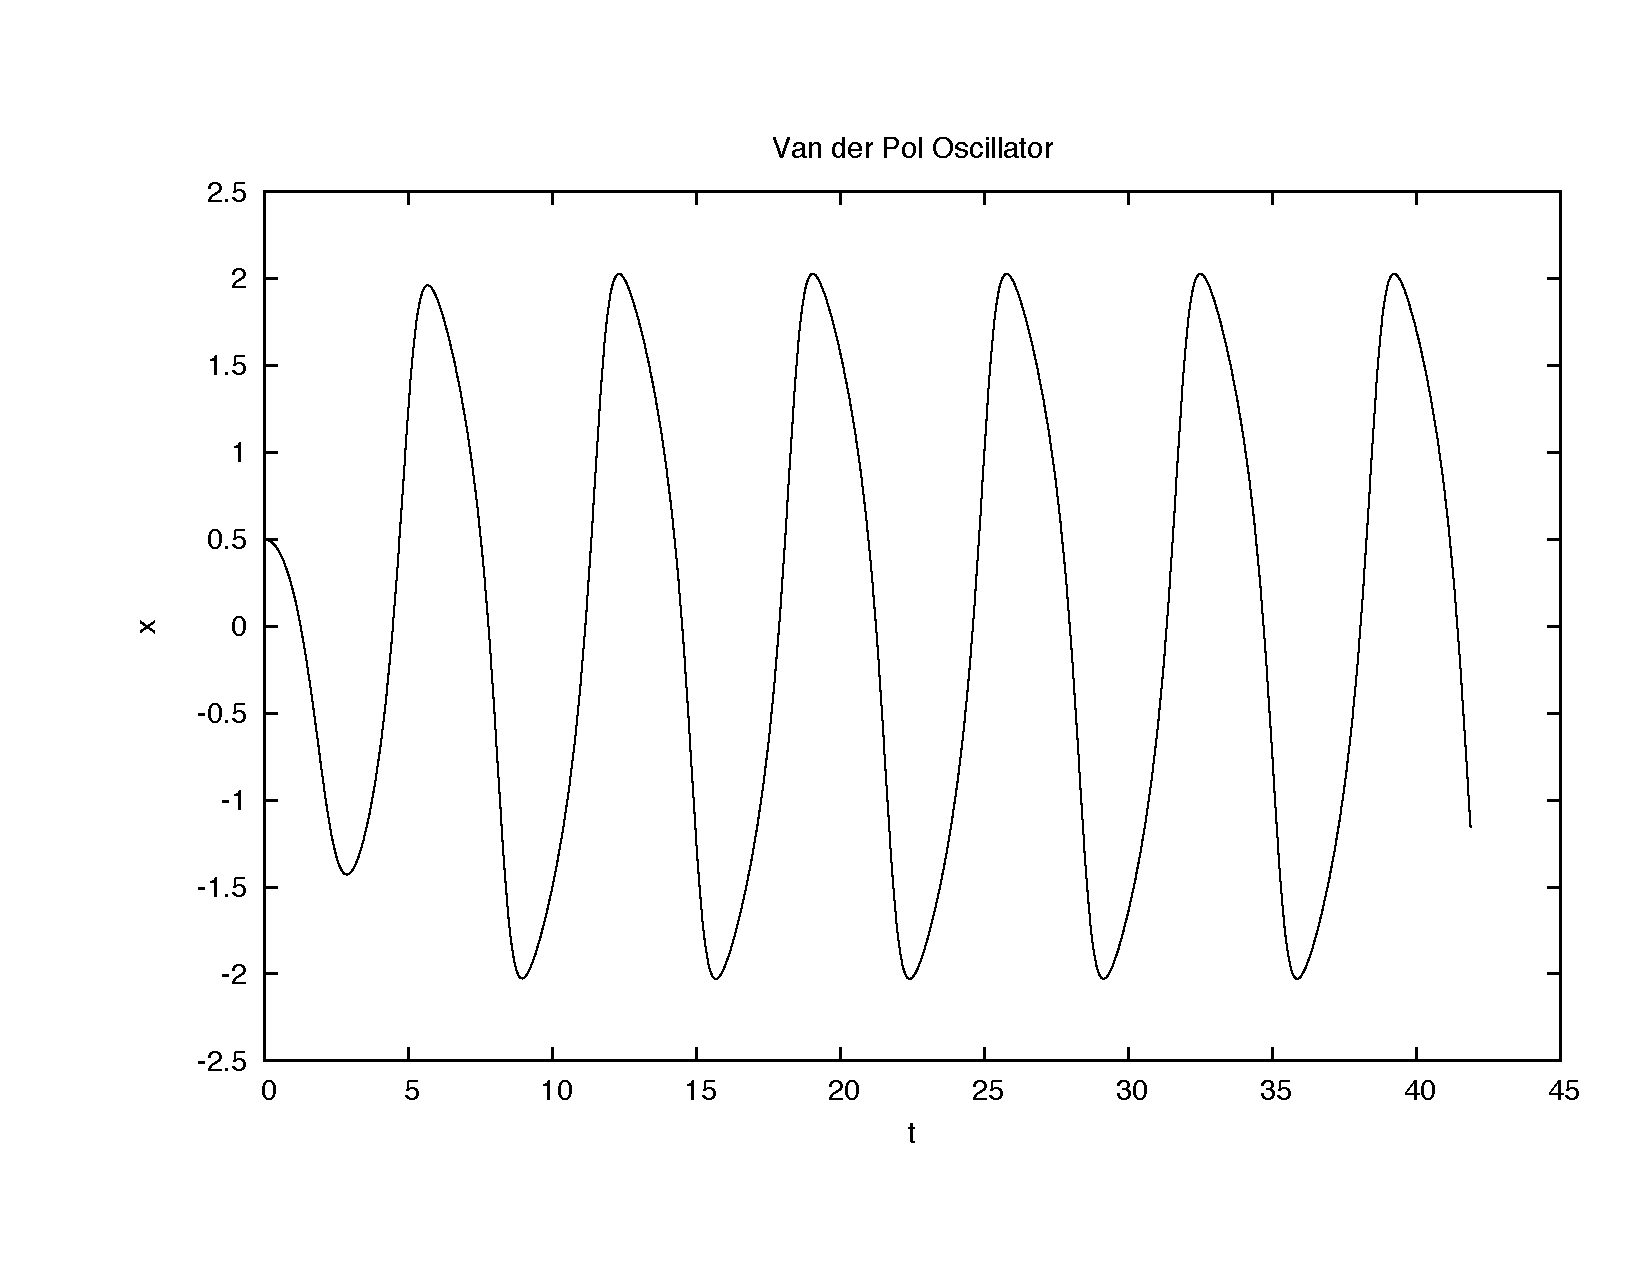
\includegraphics[width =110 mm, height = 80mm]{Fig_5_10_a.pdf}
\caption{Numeric evaluation of $x(t)$ in \eqref{van}.}
\label{fig:5_10a}
\end{figure}
\begin{figure}[!h]
\centering
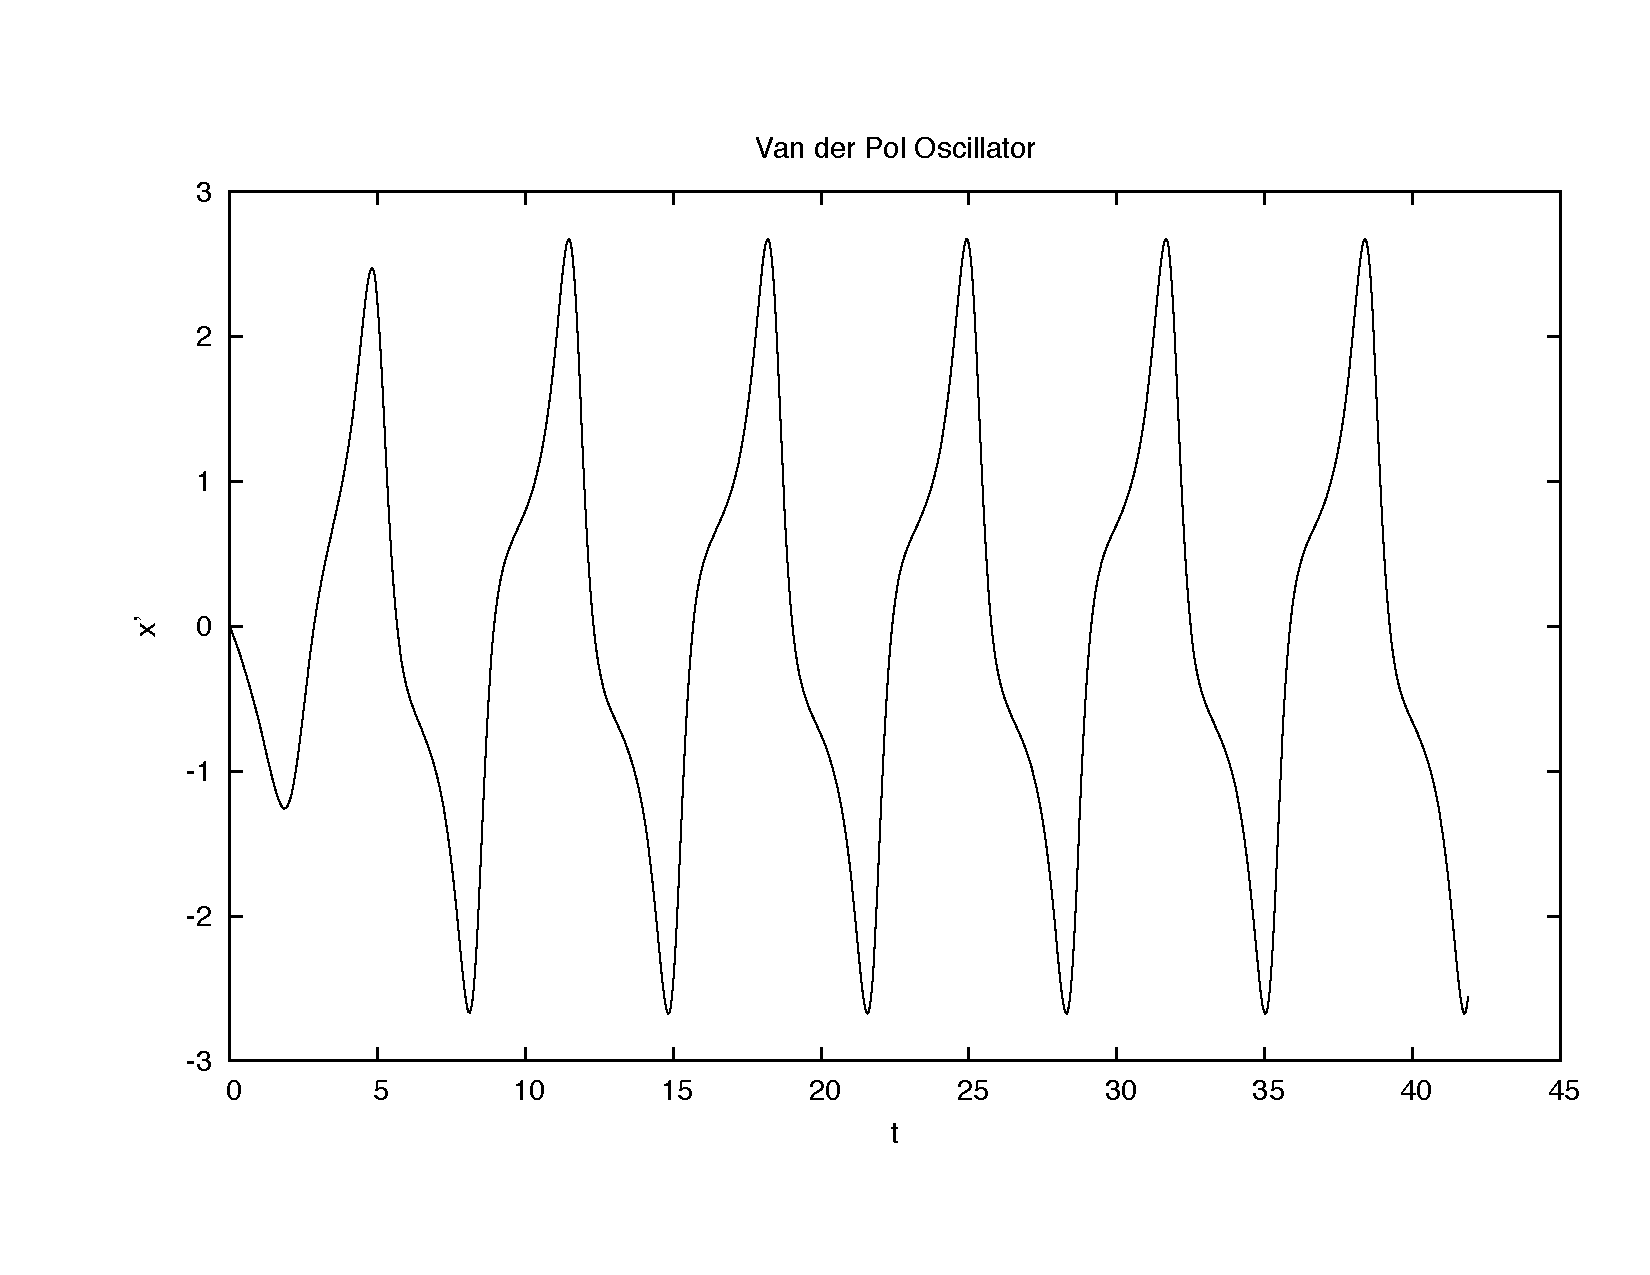
\includegraphics[width =110 mm, height = 60mm]{Fig_5_10_b.pdf}
\caption{Numeric evaluation of $\dot{x}(t)$ in \eqref{van}.}
\label{fig:5_10b}
\end{figure}
\begin{figure}[!h]
\centering
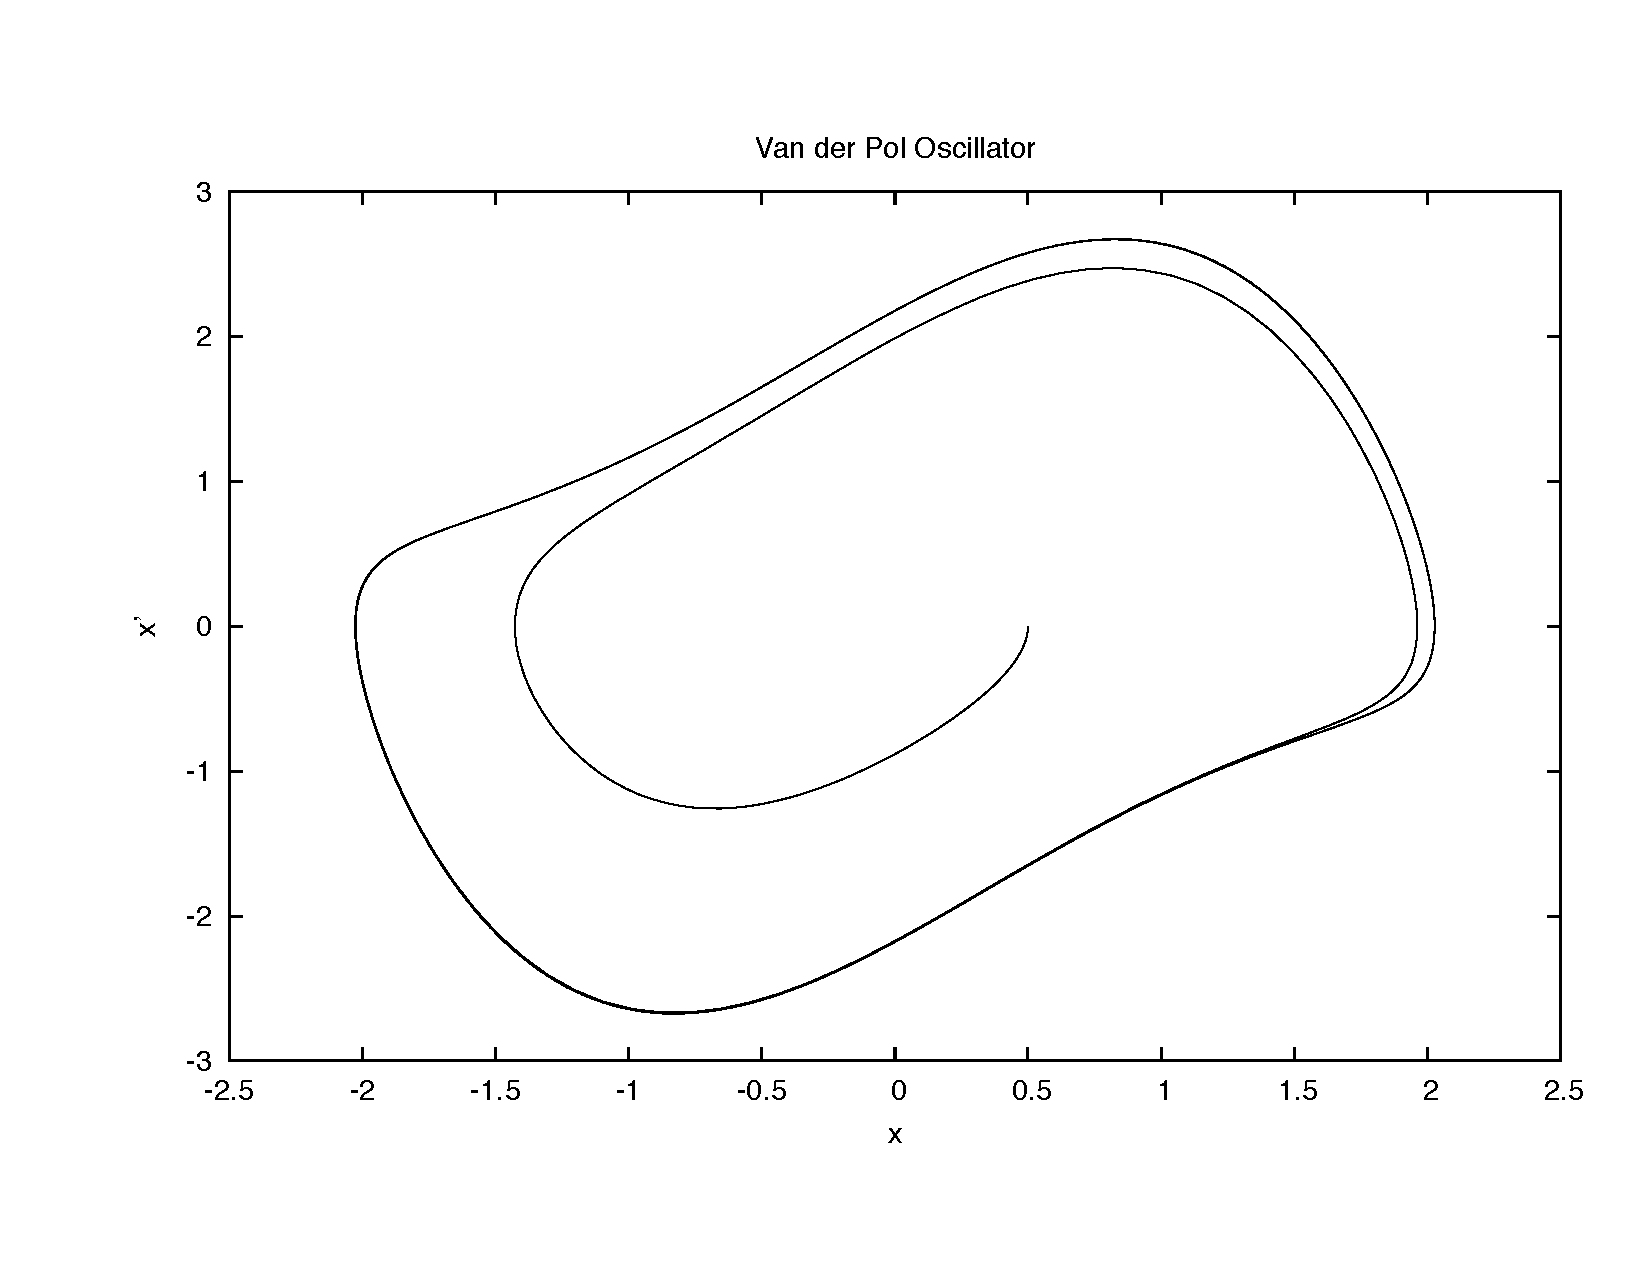
\includegraphics[width =110 mm, height = 60mm]{Fig_5_10_c.pdf}
\caption{Phase space plot of numeric evaluation of \eqref{van}.}
\label{fig:5_10c}
\end{figure}
\begin{figure}[!h]
\centering
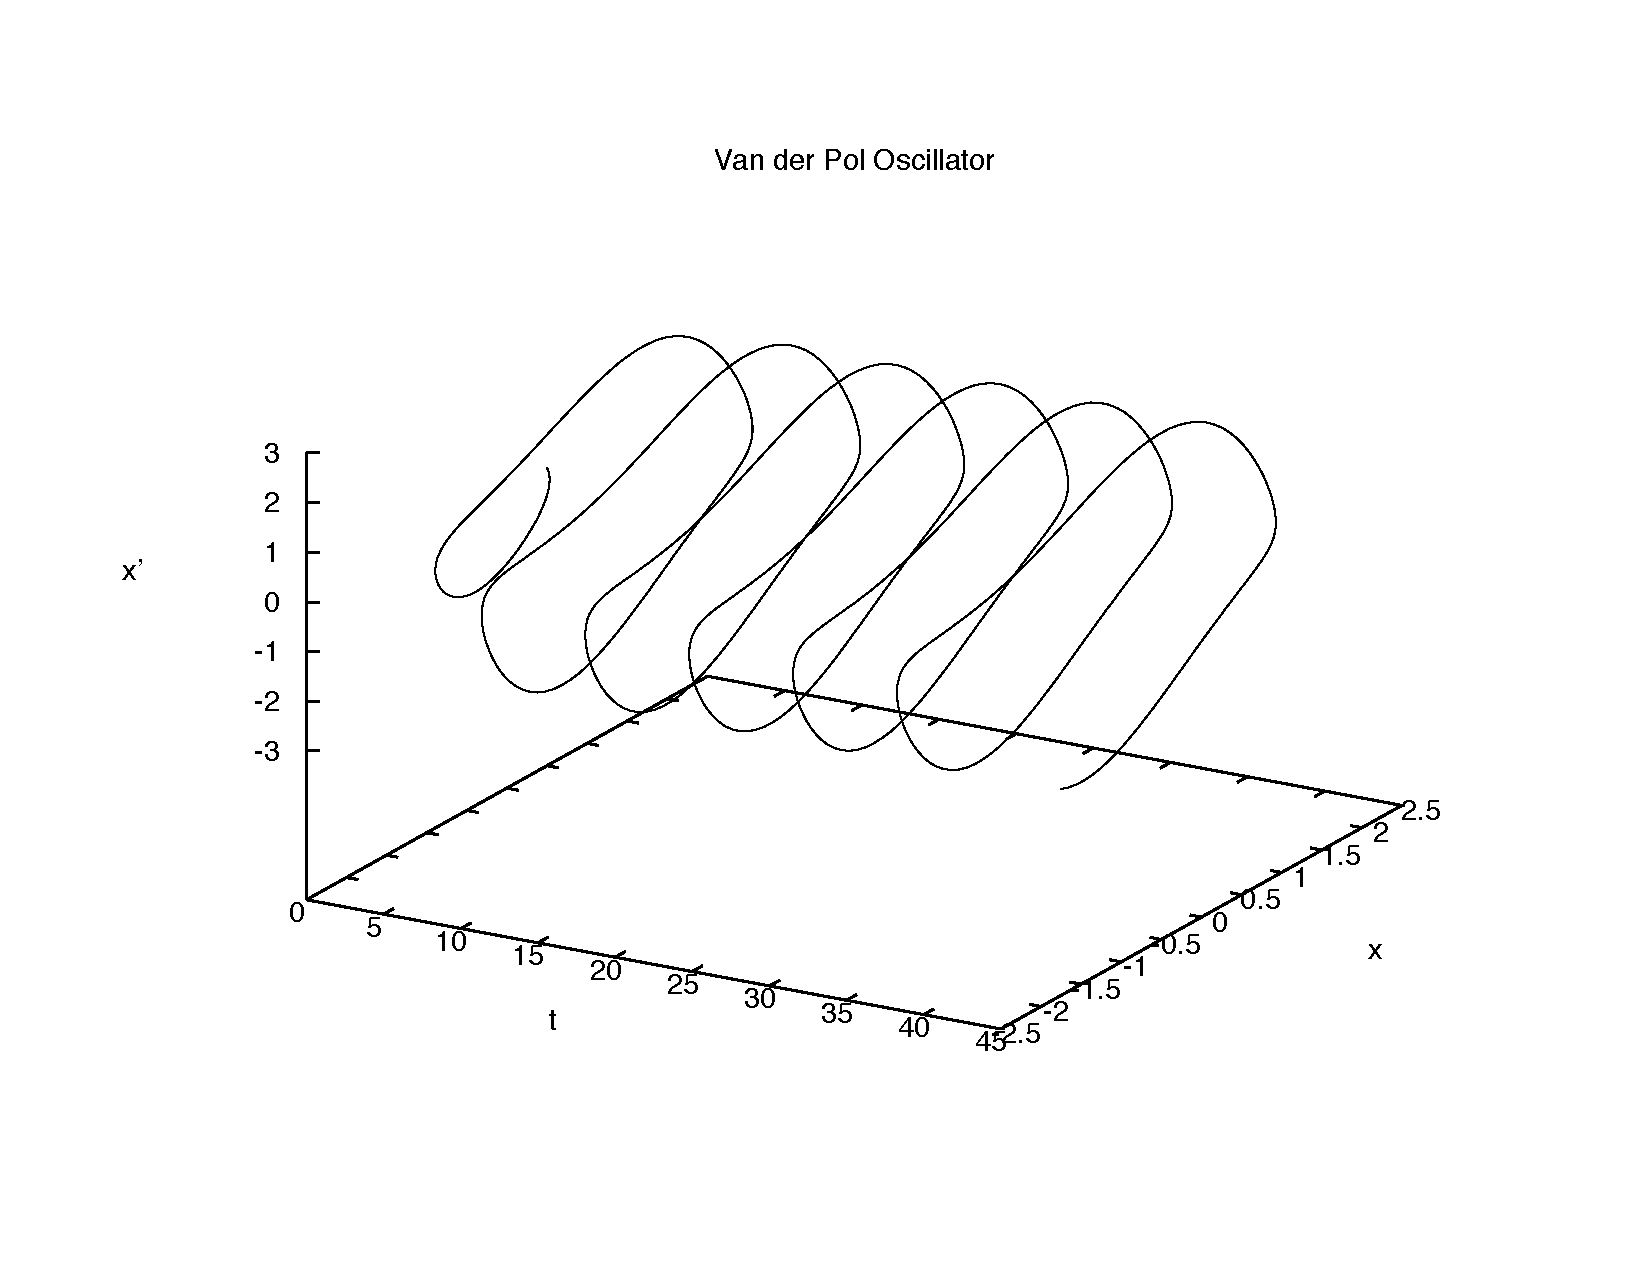
\includegraphics[width =110 mm, height = 60mm]{Fig_5_10_d.pdf}
\caption{Numeric evaluation of \eqref{van}.}
\label{fig:5_10d}
\end{figure}
\begin{figure}[!h]
\centering
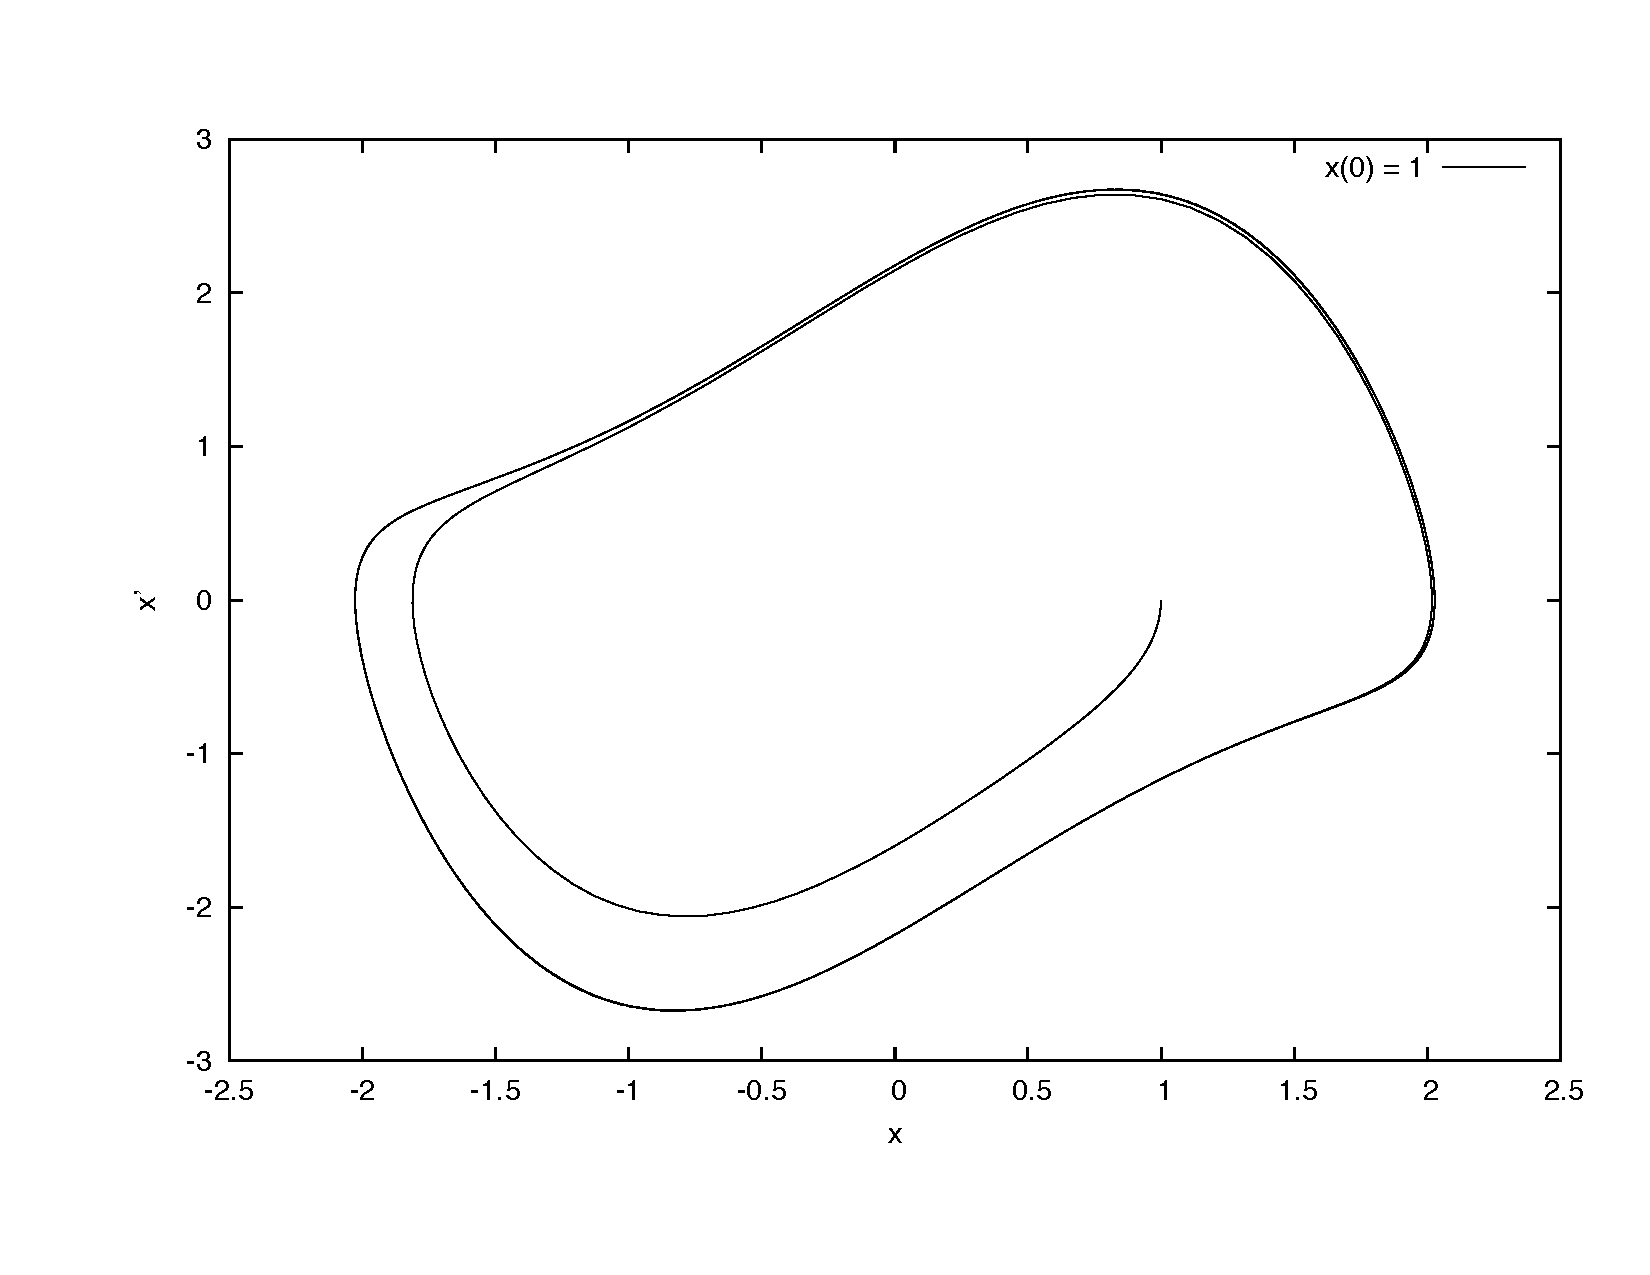
\includegraphics[width =110 mm, height = 60mm]{Ex_5_19_1.pdf}
\caption{Phase space diagram with $x(0)=1$.}
\label{fig:5_19a}
\end{figure}
\begin{figure}[!h]
\centering
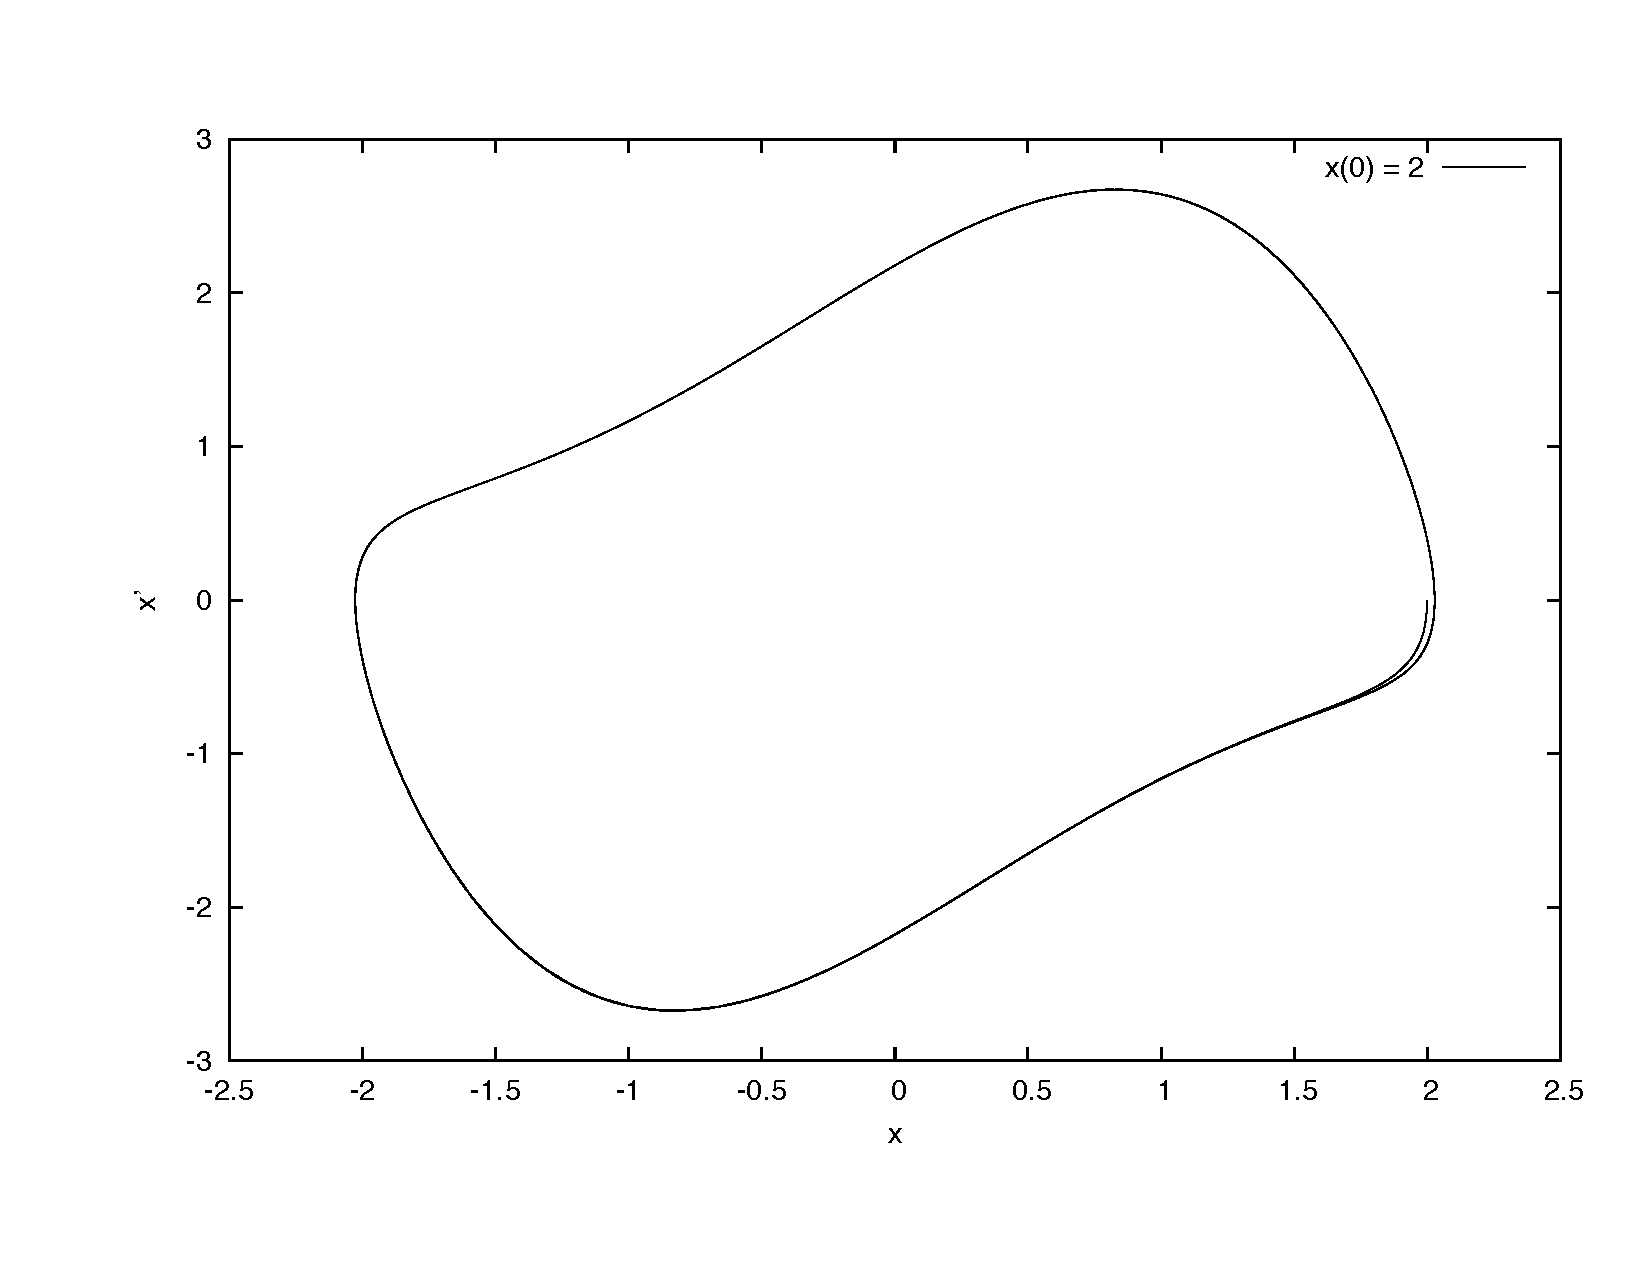
\includegraphics[width =110 mm, height = 60mm]{Ex_5_19_2.pdf}
\caption{Phase space diagram with $x(0)=2$.}
\label{fig:5_19b}
\end{figure}
\begin{figure}[!h]
\centering
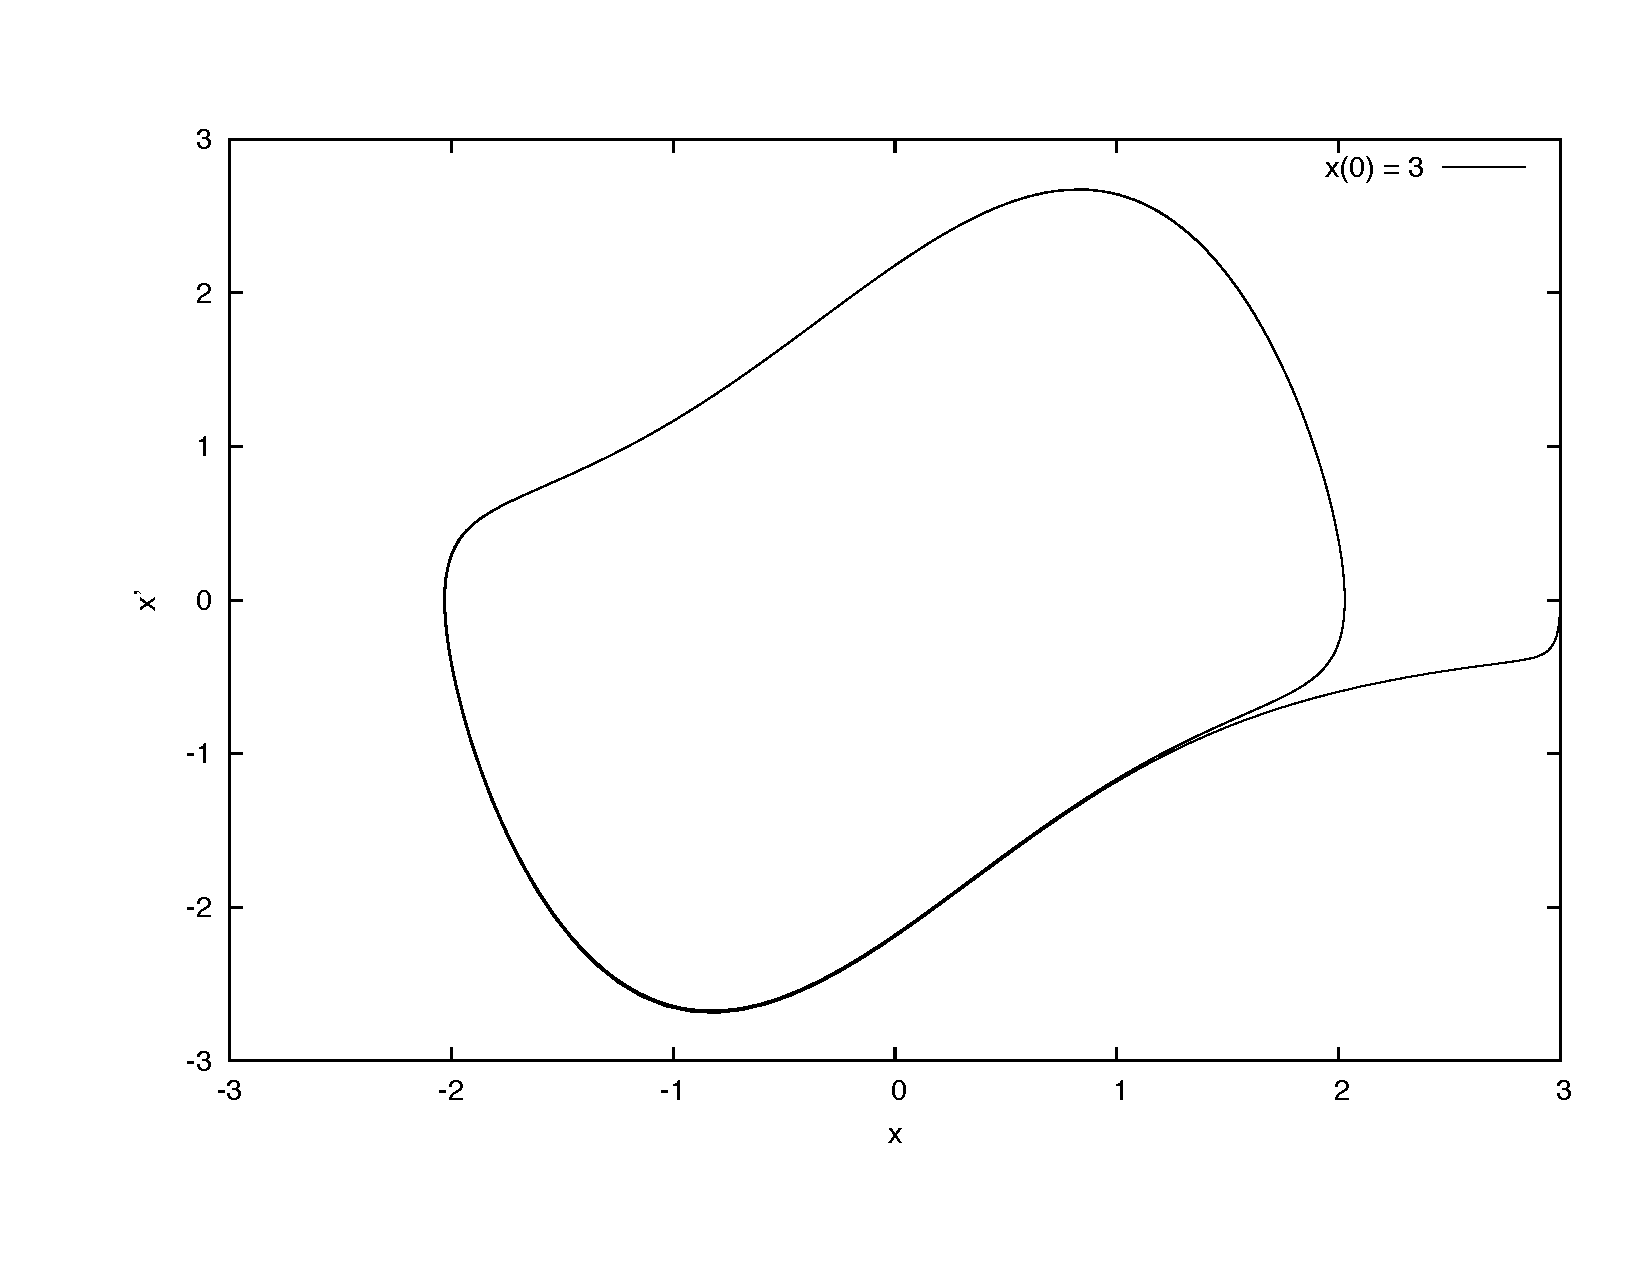
\includegraphics[width =110 mm, height = 60mm]{Ex_5_19_3.pdf}
\caption{Phase space diagram with $x(0)=3$.}
\label{fig:5_19c}
\end{figure}

Additionally, three different starting points for $x(0)$ to demonstrate the attractive properties of the phase space plot.  This series is shown in figures \ref{fig:5_19a} through \ref{fig:5_19c}.  Even though the system begins at different points, the same result occurs immediately.
\pagebreak
\subsection{Quantum Mechanics}
The final application of the RK method explored in this lab is the analysis of two quantum mechanical potentials:
\begin{equation}
\label{v1}
V(x)=x^2
\end{equation}
\begin{equation}
\label{v2}
V(x)=|x|
\end{equation}
The first potential, the harmonic oscillator, has been very thoroughly studied and can be solved analytically with little effort.  Unfortunately, this relatively simple problem caused enormous problems for the code developed in this lab.  The wave functions could not be successfully generated for this potential system and the energy values returned that were associated with them were also incorrect.

The application of the second potential generated much more successful results.  The first five wave function are shown below in figures \ref{fig:quant1} through \ref{fig:quant5}.  The first order wave function has an error in that $\psi(x)$ approaches negative infinity as $x$ gets large.  This is a result of the boundary condition only being applied to the initial $x$ value and not at both ends of the well.  The energy values for this potential system were also calculated, shown in Table 1.
\begin{center}
Table 1:  Energy of \eqref{v2} \\
\begin{tabular}{ | c | c |}
\hline
N & Energy \\ \hline
1&	-107623.894705 \\ \hline
2&	131.270440 \\ \hline
3&	-26.452375 \\ \hline
4&	1.399143 \\ \hline
5&	-0.428047 \\ \hline
\end{tabular}
\end{center}
It is clear that the energy for the first wave function is incorrect, which is to be expected due to the error in the wave function, itself.  Since no analytic or standard values were provided, it is quite difficult to comment on the accuracy of these results.  The apparent oscillation between positive and negative values would indicate a potential error, but more data is required to make a meaningful conclusion.  A graphical analysis of the wave functions generated with this code yields promising observations.  One sees that, in all cases but the first order, the wave functions decay away exponentially in the region that would be classically forbidden.  Additionally, there is the expected oscillations in the allowed region.
\begin{figure}[!h]
\centering
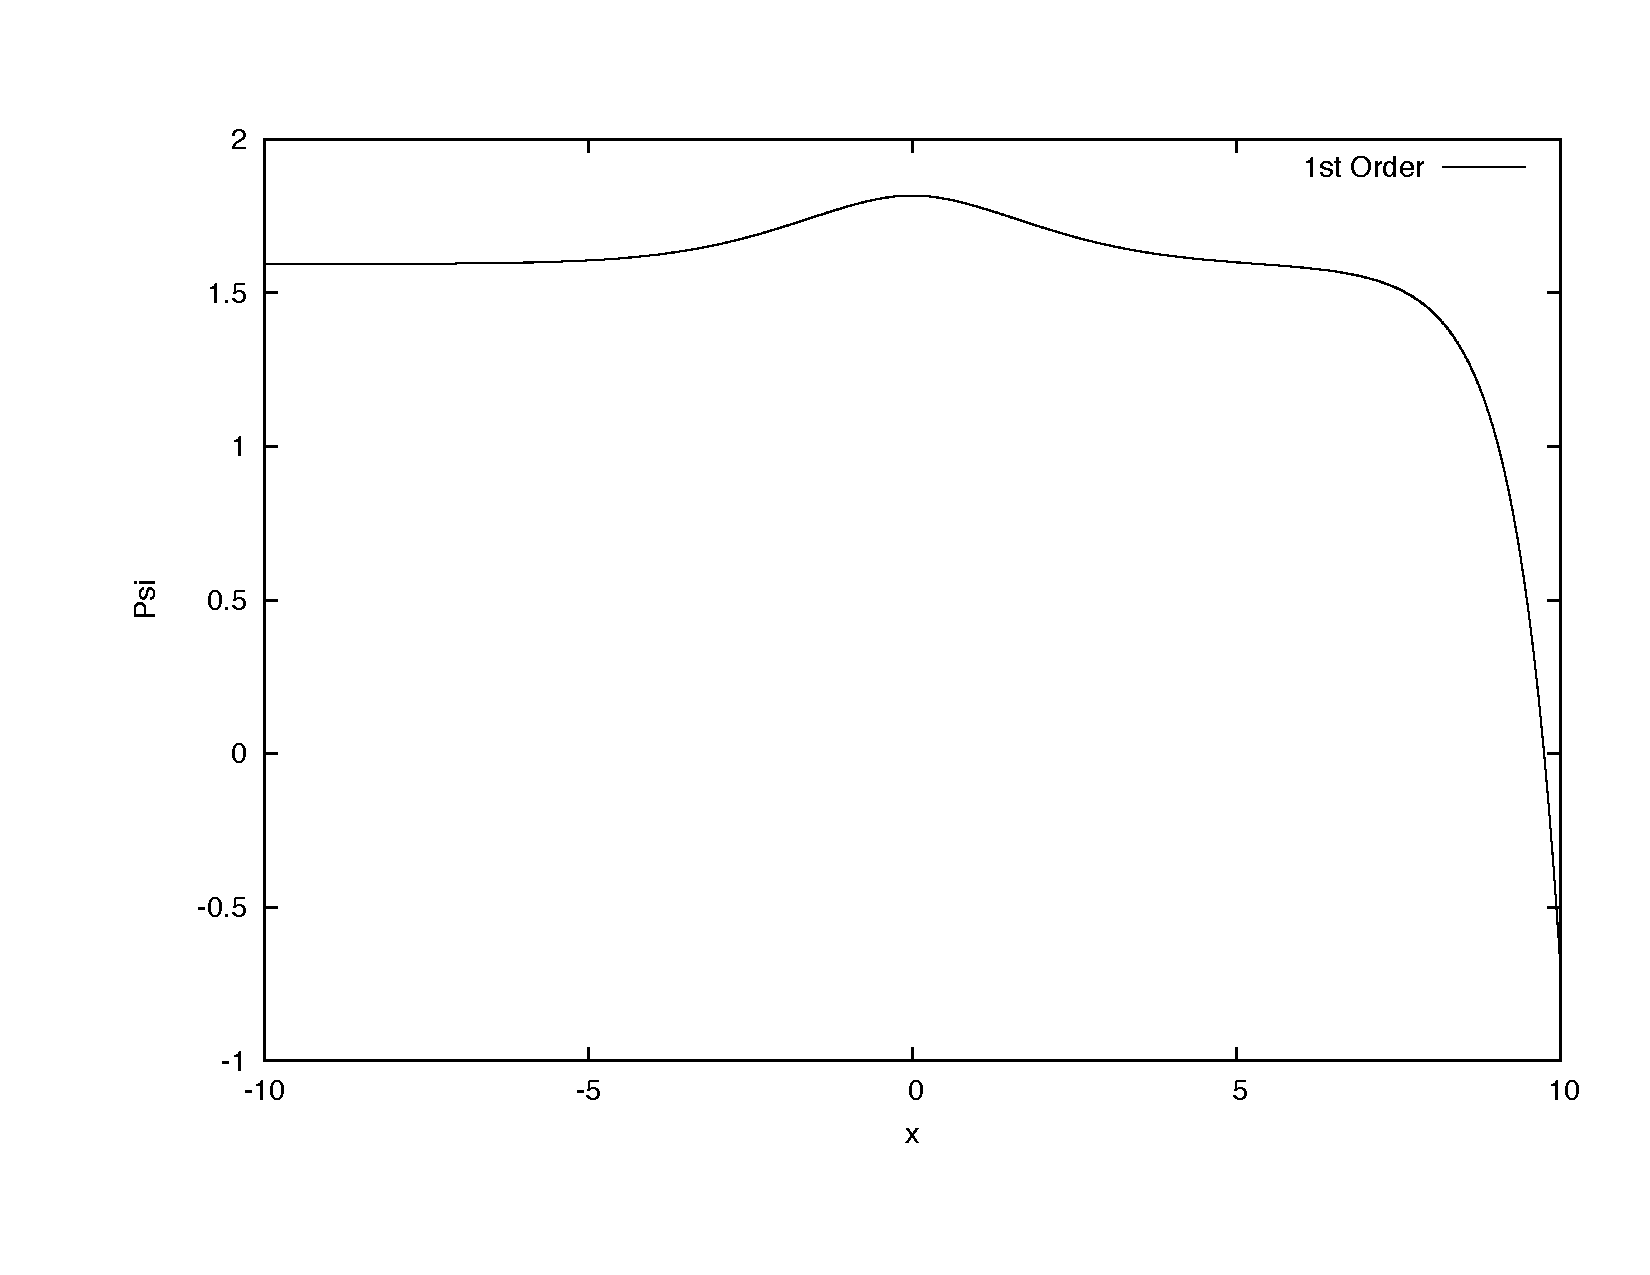
\includegraphics[width =110 mm, height = 45mm]{quantum_abs_1.pdf}
\caption{First order wave function for the \eqref{v2}.}
\label{fig:quant1}
\end{figure}
\begin{figure}[!h]
\centering
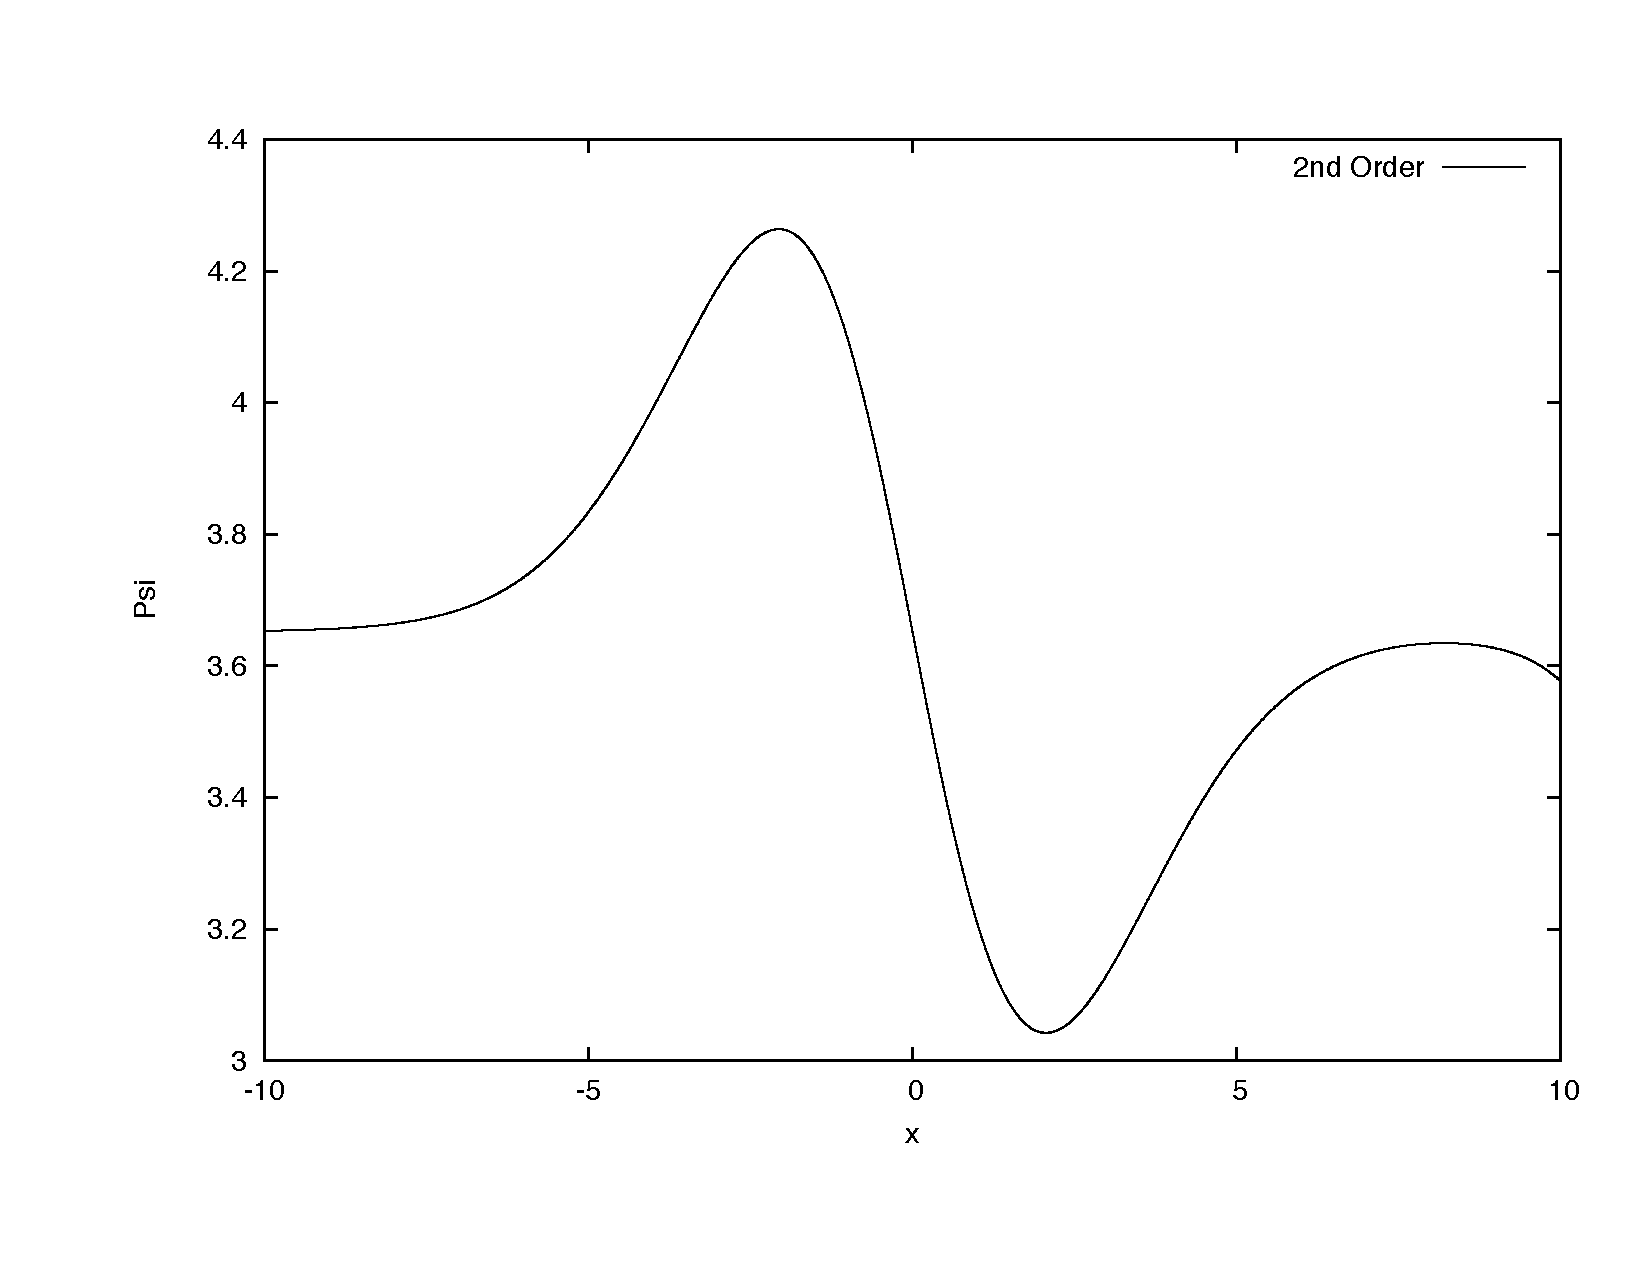
\includegraphics[width =110 mm, height = 60mm]{quantum_abs_2.pdf}
\caption{Second order wave function for the \eqref{v2}.}
\label{fig:quant2}
\end{figure}
\begin{figure}[!h]
\centering
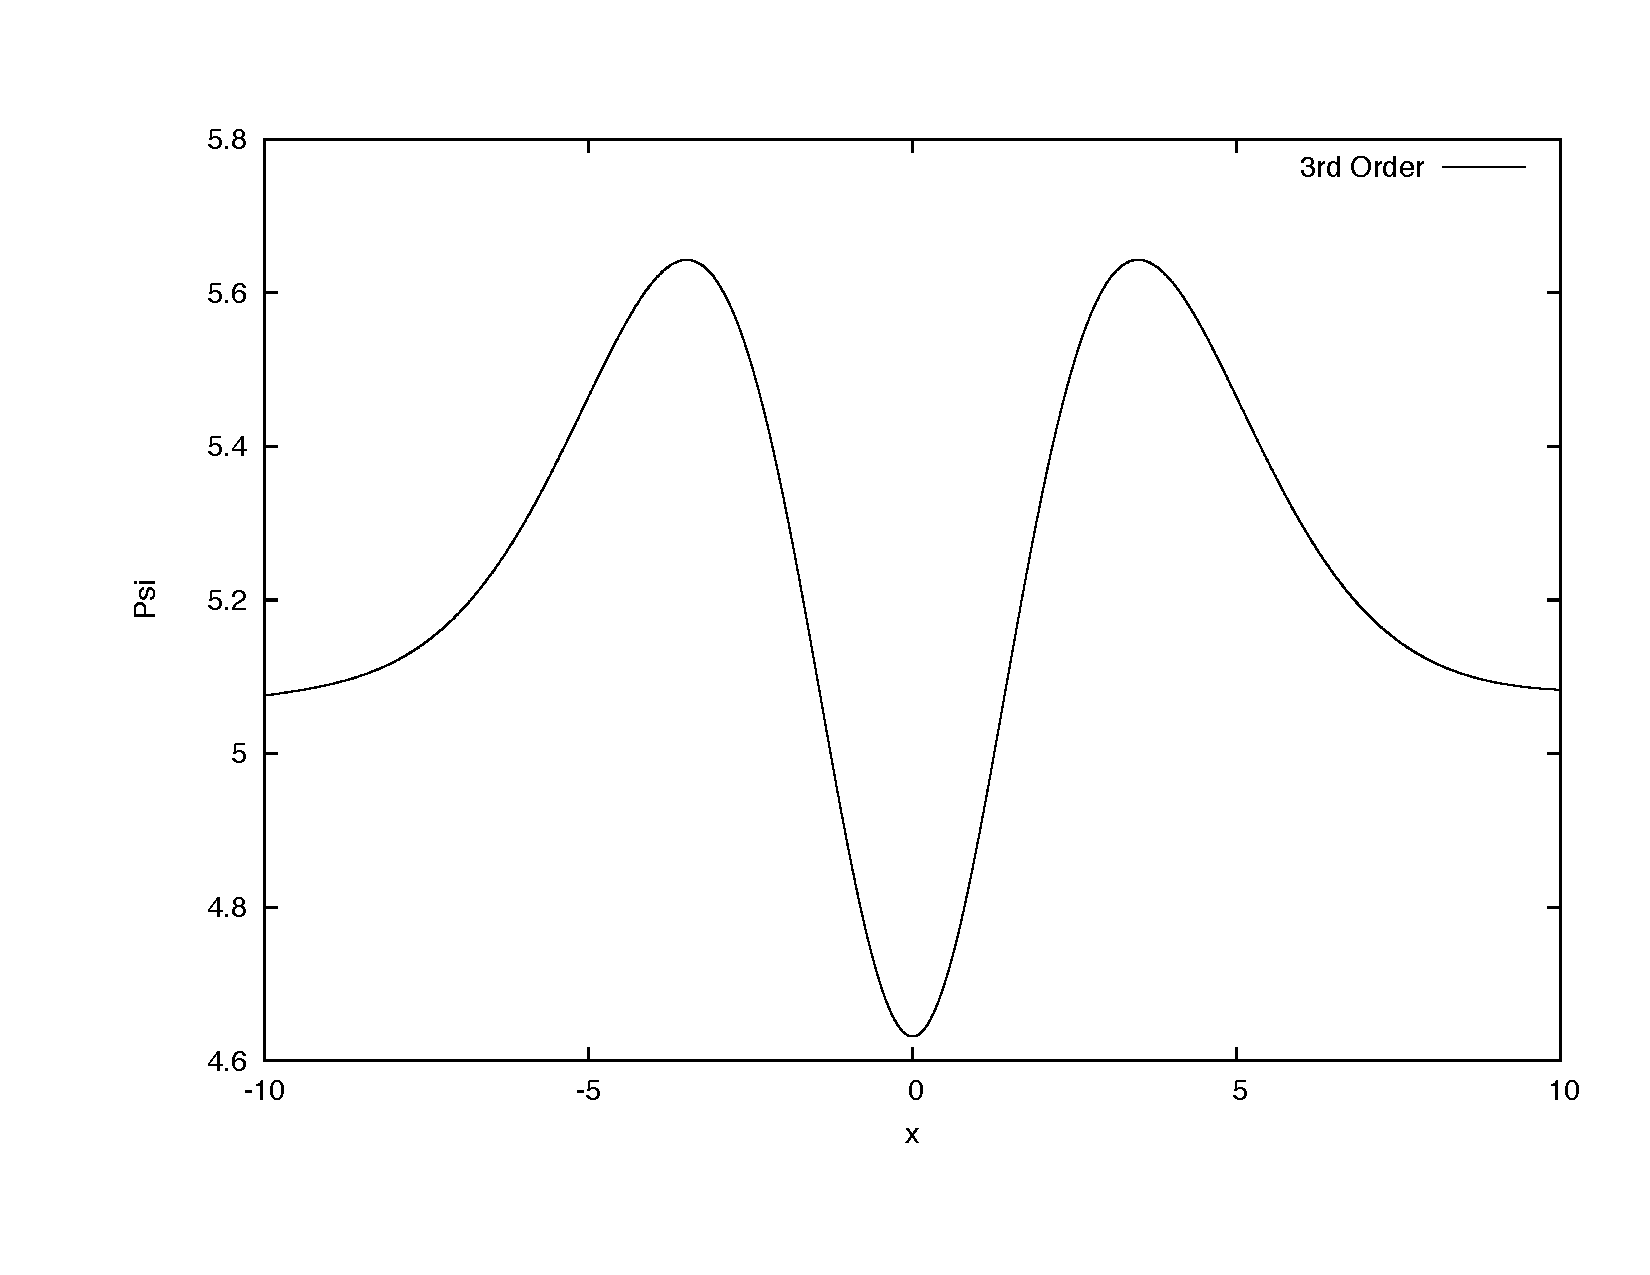
\includegraphics[width =110 mm, height = 60mm]{quantum_abs_3.pdf}
\caption{Third order wave function for the \eqref{v2}.}
\label{fig:quant3}
\end{figure}
\begin{figure}[!h]
\centering
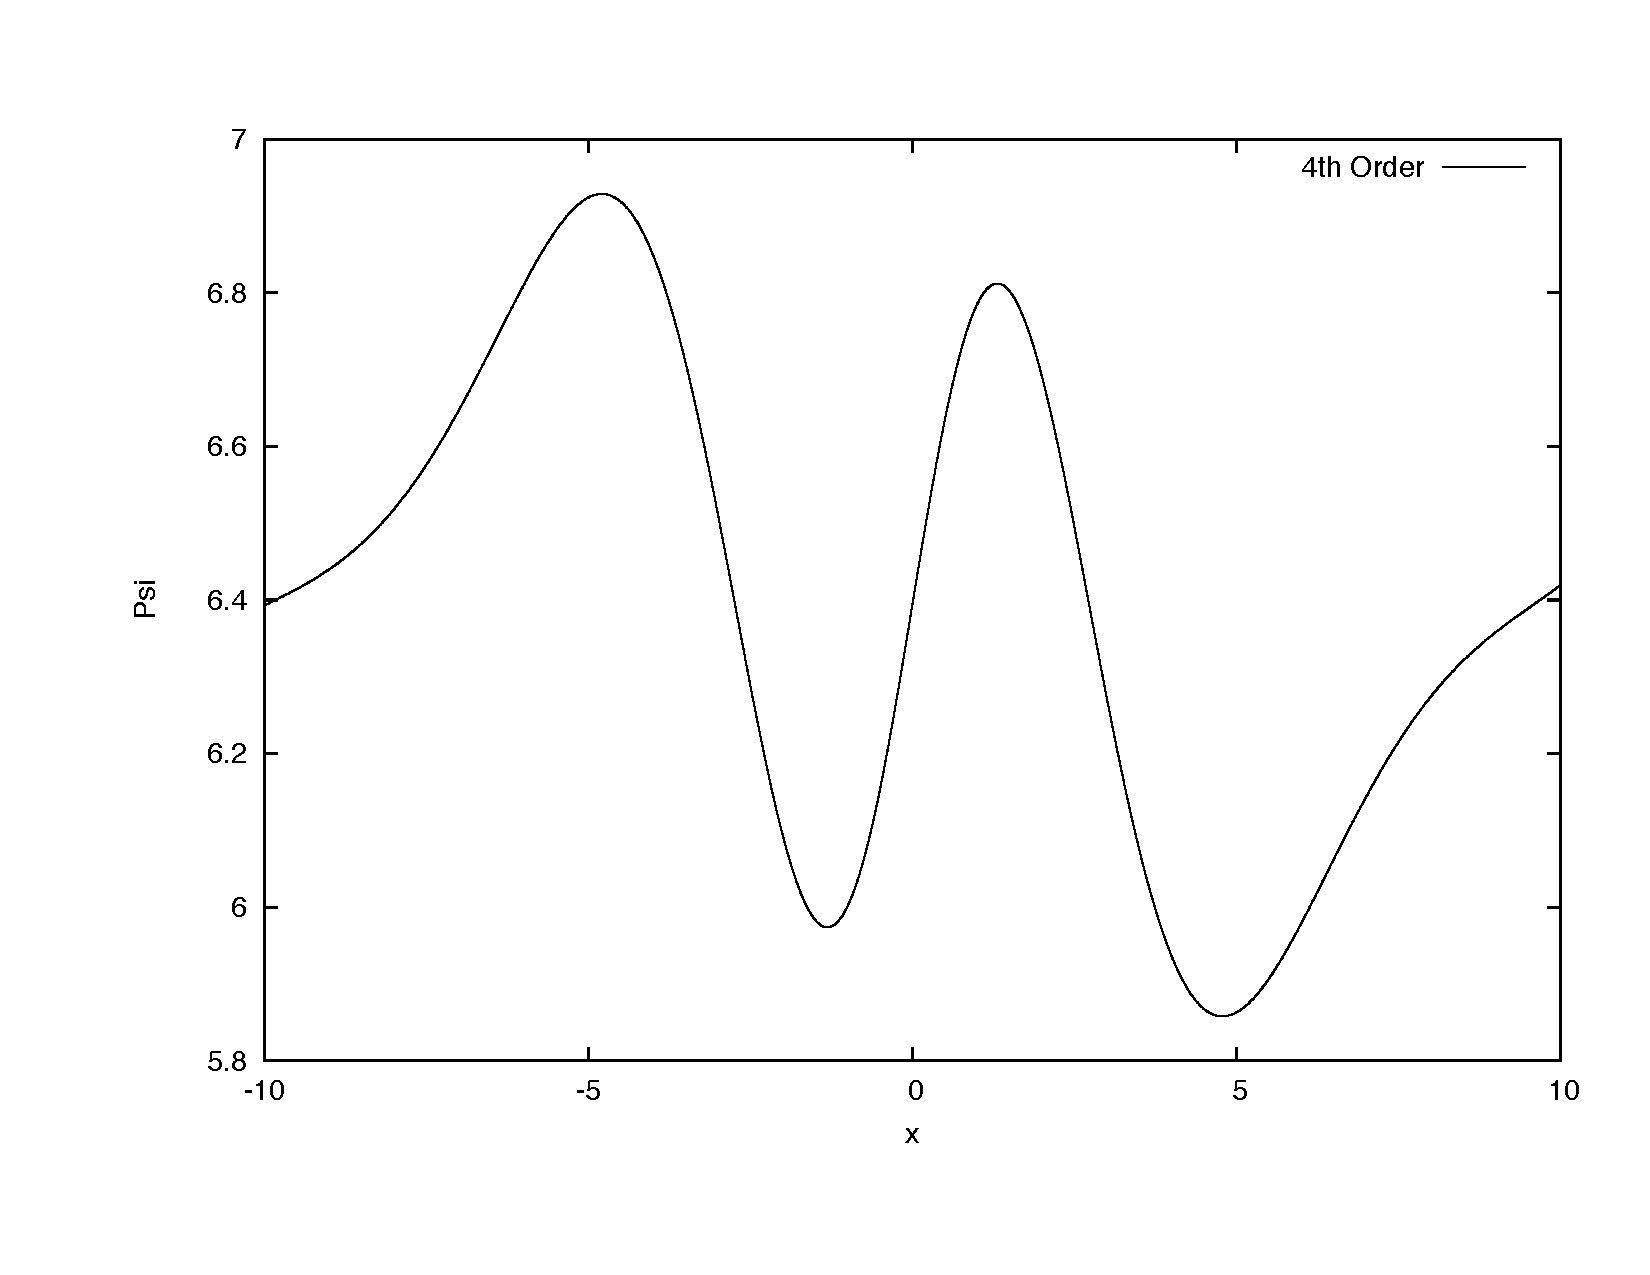
\includegraphics[width =110 mm, height = 60mm]{quantum_abs_4.pdf}
\caption{Fourth order wave function for the \eqref{v2}.}
\label{fig:quant4}
\end{figure}
\begin{figure}[!h]
\centering
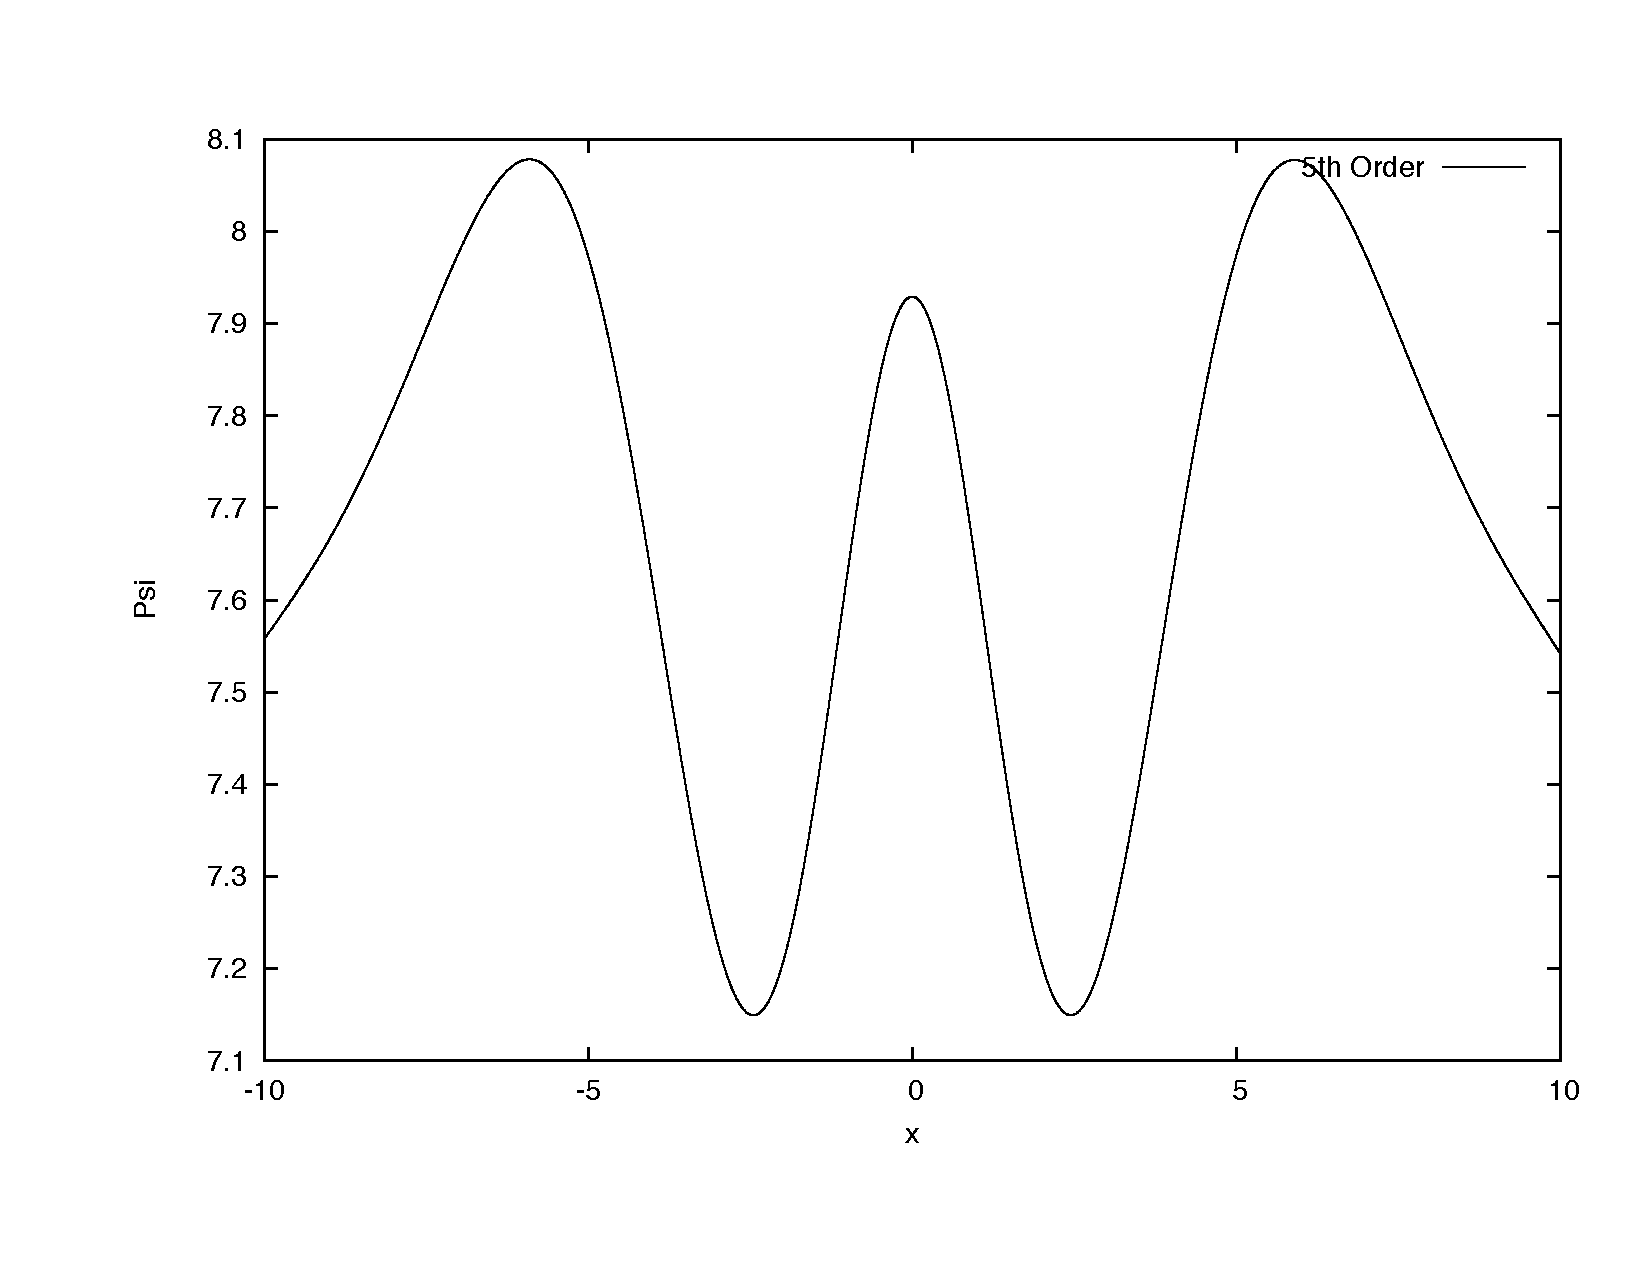
\includegraphics[width =110 mm, height = 60mm]{quantum_abs_5.pdf}
\caption{Fifth order wave function for the \eqref{v2}.}
\label{fig:quant5}
\end{figure}
\pagebreak
\subsection{Exercise 5.33}
The first application of the finite difference technique was the analysis of a simple differential equation
\begin{equation}
\label{533}
y''(x)-5y'(x)+10y(x)=10x
\end{equation}
with the initial conditions $y(0)=0$ and $y(1)=100$.
\begin{center}
Table 2:  Solution to \eqref{533} \\
\begin{tabular}{ | c | c |}
\hline
$x$ & $y(x)$ \\ \hline
0.0&	0.000000000000000 \\ \hline
0.1&	1.868039343425737 \\ \hline
0.2&	4.761292691344755 \\ \hline
0.3&	9.002066522620158 \\ \hline
0.4&	14.949257041676869 \\ \hline
0.5&	22.973326710040435 \\ \hline
0.6&	33.412203844890676 \\ \hline
0.7&	46.501233590674303 \\ \hline
0.8&	62.269332700293980 \\ \hline
0.9&	80.392982039667089 \\ \hline
1.0&	100.000000000000000 \\ \hline
\end{tabular}
\end{center}
These results match those found in Devries' Computation Physics text book to a high accuracy (~5\%).  These results were obtained by allowing a linear solution between $y(0)$ and $y(1)$ 'relax' down into the proper values seen above.
\subsection{Piano Wire}
The next application of the finite difference method was the analysis of the fundamental frequencies of vibration in a nonuniform piano wire.  Beginning with the standard wave equation
\begin{equation}
\label{wave}
\frac{\partial^2u(x,t)}{\partial t^2}=\frac{T}{\mu(x)} \frac{\partial^2 u(x,t)}{\partial x^2}
\end{equation}
one can substitute \eqref{finitey''} into \eqref{wave} to find
\begin{equation}
\label{wave2}
\frac{T}{\mu_i} \frac{y_{i+1}-2y_i+y_{i-1}}{h^2}+\omega^2 y_i=0
\end{equation}
By making use of the fixed ends, one can develop a matrix equation of form
\begin{equation}
\label{mat}
\mathbf{A x} = \lambda \mathbf{x}
\end{equation}
where $\lambda = \omega^2$ and 

\[
\begin{bmatrix}
-2\frac{T}{\mu_1 h^2} & \frac{T}{\mu_1h^2} &0 & & \\
\frac{T}{\mu_2 h^2} & -2\frac{T}{\mu_2 h^2} & \frac{T}{\mu_2 h^2}& & \\
 & \ddots&\ddots & \ddots & & \\
 & & \frac{T}{\mu_{N-2} h^2} & -2\frac{T}{\mu_{N-1} h^2}& \frac{T}{\mu_{N-1} h^2} \\
 & & & \frac{T}{\mu_N h^2} & -2\frac{T}{\mu_1 h^2} \\  
\end{bmatrix}
  =
\mathbf{A} \]
\[
\begin{bmatrix}
f_1\\
f_2\\
\vdots \\
f_{N-1}\\
f_N\\
\end{bmatrix}
  =
\mathbf{x} \]
A method for developing the solution of matrices of this form was developed in the previous lab, so completing this problem was a simple process.  A varying mass density was used that had the following form
\begin{equation}
\label{mu}
\mu(x)= \mu_0 + (x - \frac{L}{2})\Delta
\end{equation}
The parameters for this system were set to $\mu_0 = 0.954$, $L=1$, $T=1000$, $\Delta=0.5$, and $dt=1e-3$.  Table 3 shows the eigenvalues generated.
\begin{center}
Table 2:  Eigenvalues of \eqref{mat} \\
\begin{tabular}{ | c |}
\hline
1.001001502504383 \\ \hline
2.002003005008766 \\ \hline
3.011334633106239 \\ \hline
4.010257389327687 \\ \hline
5.010010020030060 \\ \hline
6.010178407416700 \\ \hline
7.014156884015866 \\ \hline
\end{tabular}
\end{center}
these values are expressed in multiples of the fundamental frequency:
\begin{equation}
\label{f0}
f_0=\frac{\pi}{L}\sqrt{\frac{T}{\mu_0}}
\end{equation}
The fact that the low order eigenvalues are essentially interval multiples of $f_0$ lends support to these results.

This problem was further explored by studying the effects of putting a Gaussian 'bump' in the center of the wire and observing the time evolution.
\begin{equation}
\label{gauss}
u(x,0)= e^{-100(x-0.5)^2} , 0<x<1
\end{equation}
Using a time step of $dt=1e-4$, the following series of snapshots were taken.
\begin{figure}[!h]
\centering
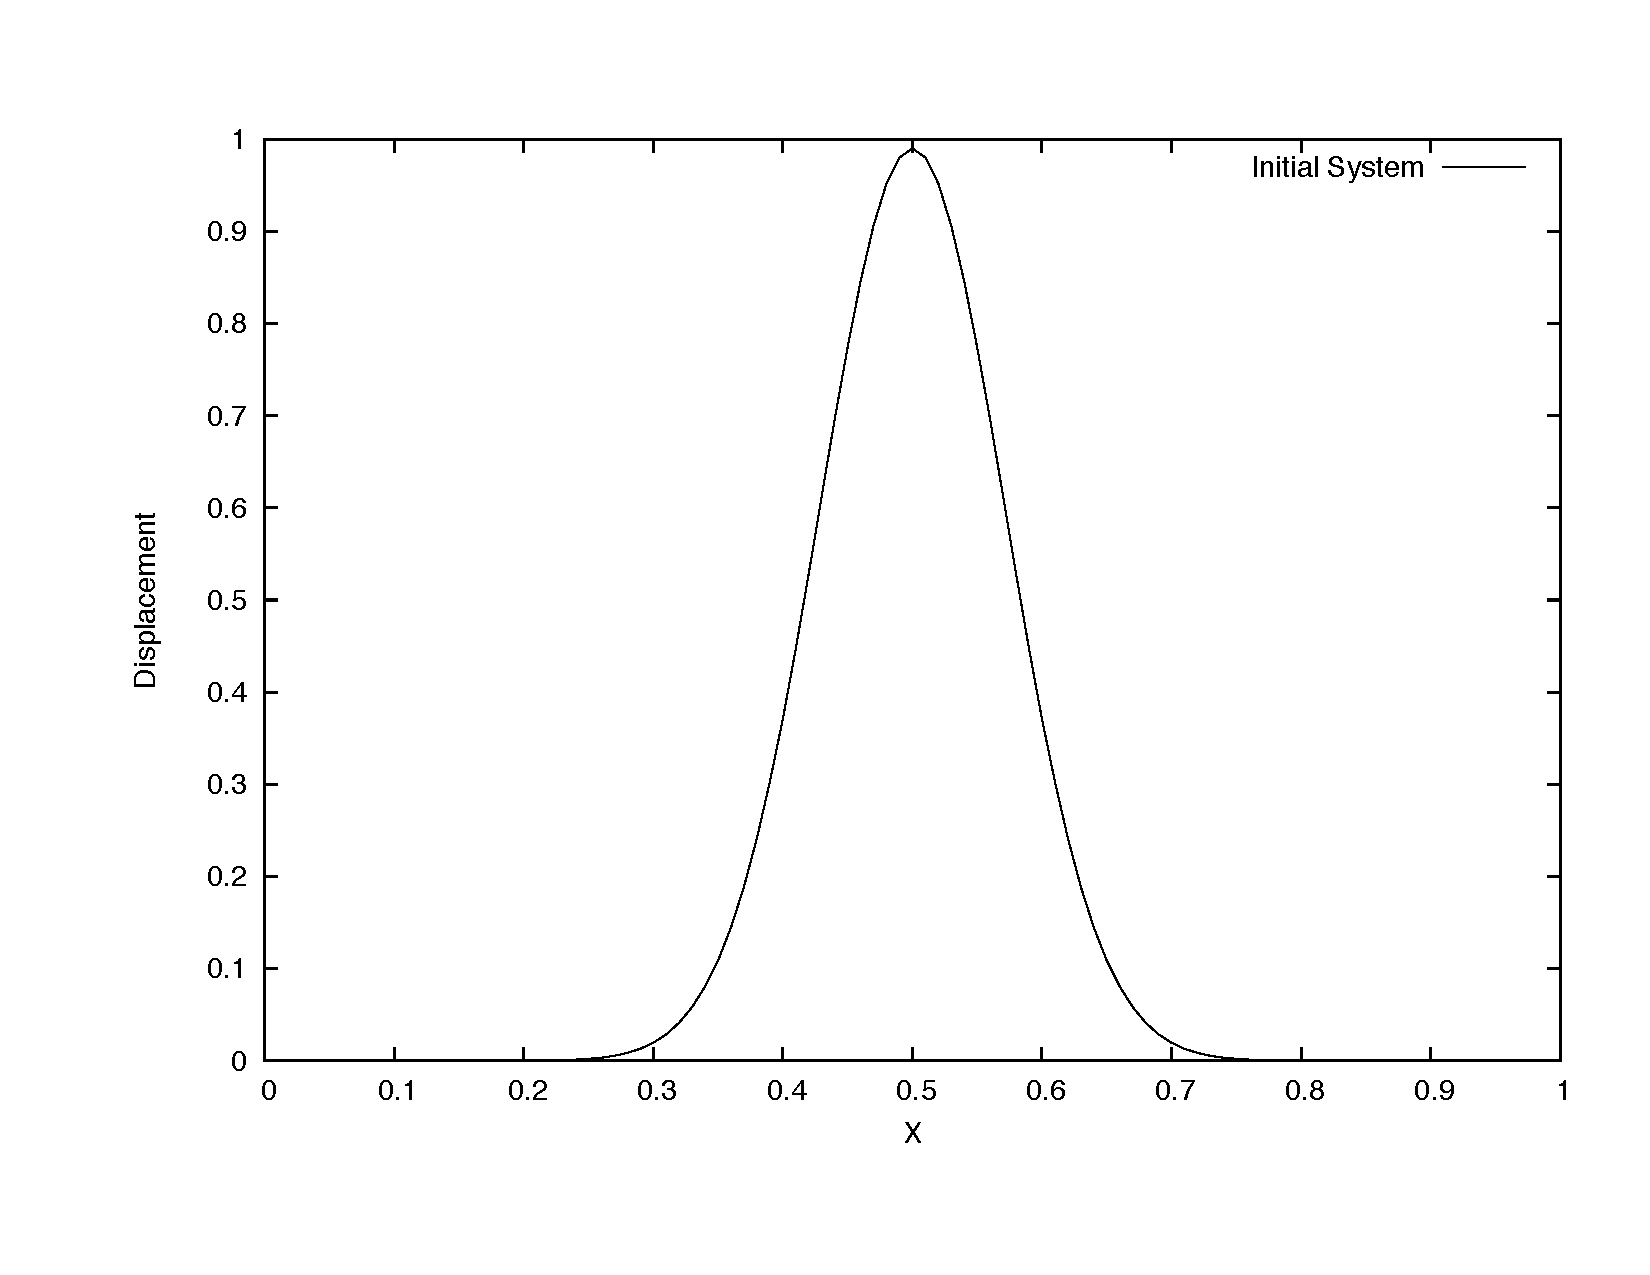
\includegraphics[width =110 mm, height = 50mm]{Ex_7_1_0.pdf}
\caption{Initial state of the 'bumped' piano wire.}
\label{fig:7_1_0}
\end{figure}
\begin{figure}[!h]
\centering
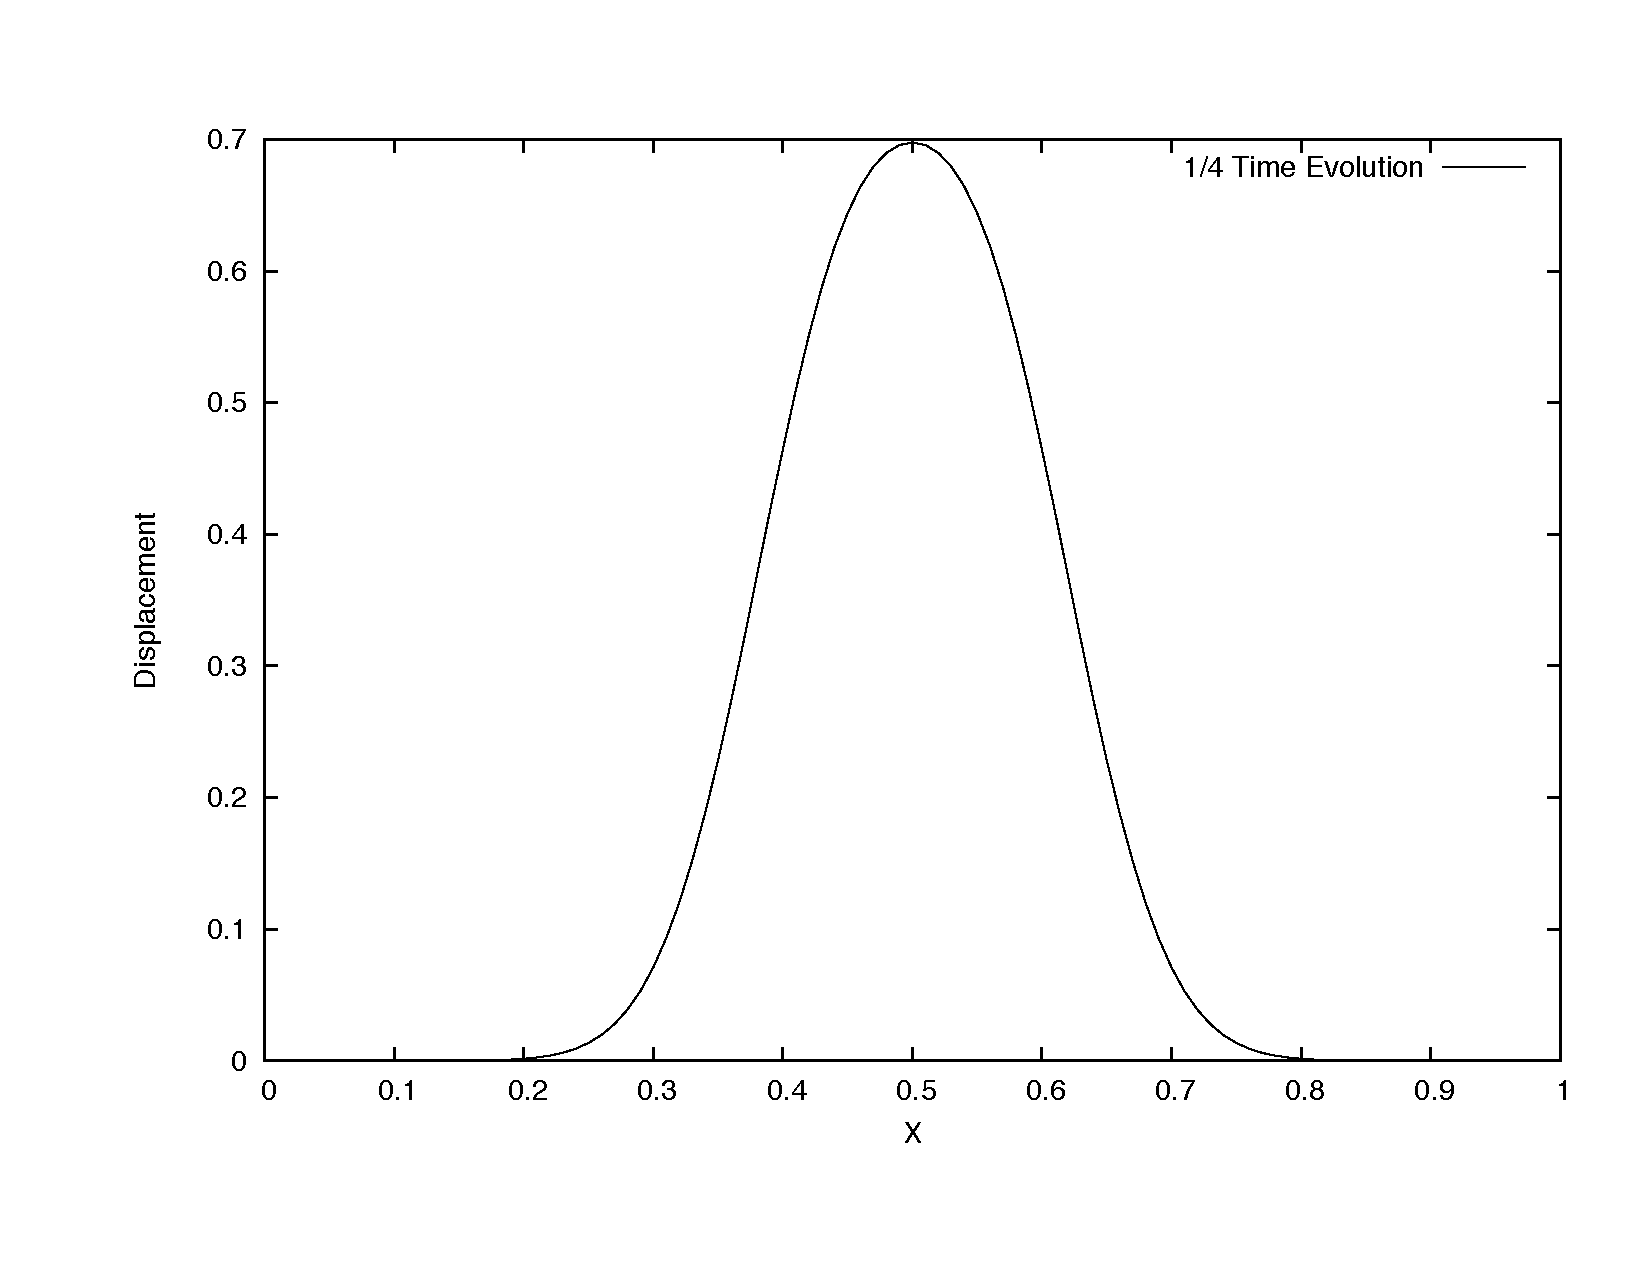
\includegraphics[width =110 mm, height = 50mm]{Ex_7_1_25.pdf}
\caption{'Bumped' piano wire after 1/4 time evolution.}
\label{fig:7_1_25}
\end{figure}
\begin{figure}[!h]
\centering
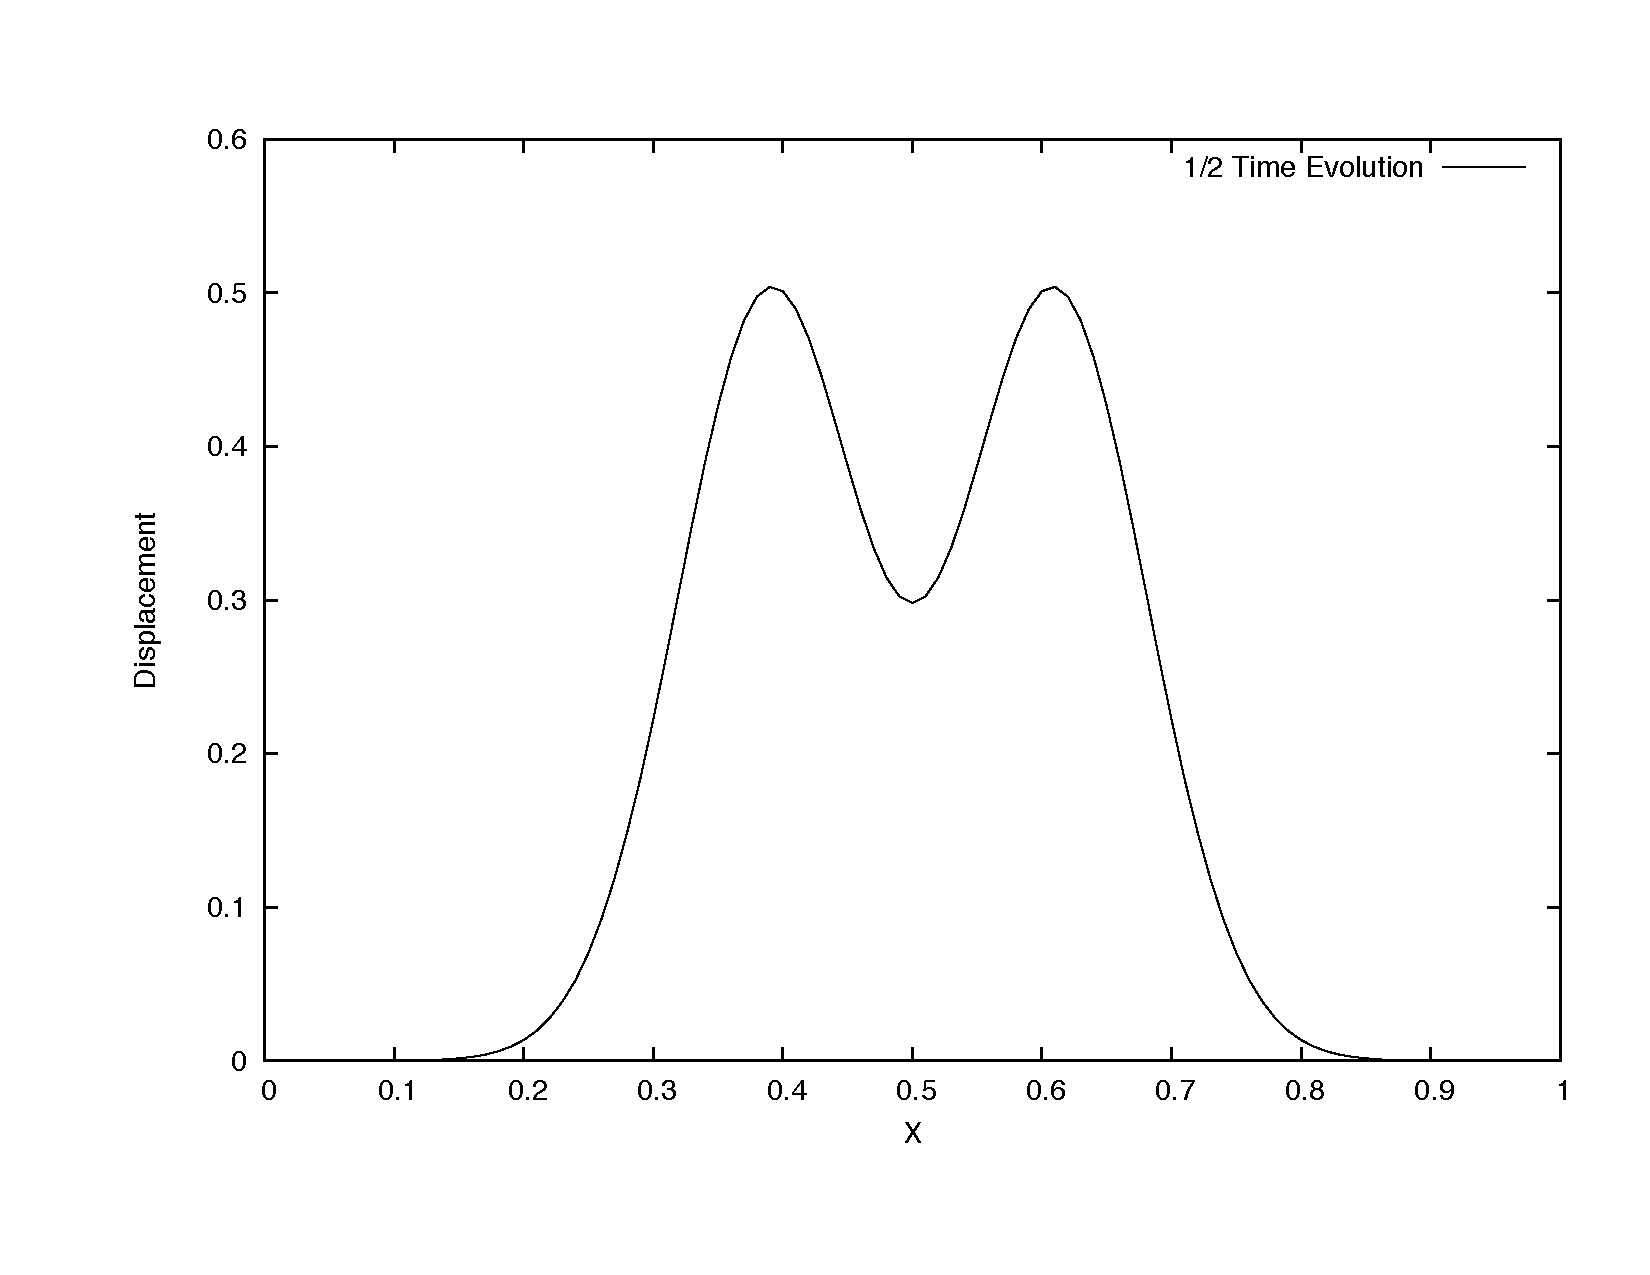
\includegraphics[width =110 mm, height = 60mm]{Ex_7_1_50.pdf}
\caption{'Bumped' piano wire after 1/2 time evolution.}
\label{fig:7_1_50}
\end{figure}
\begin{figure}[!h]
\centering
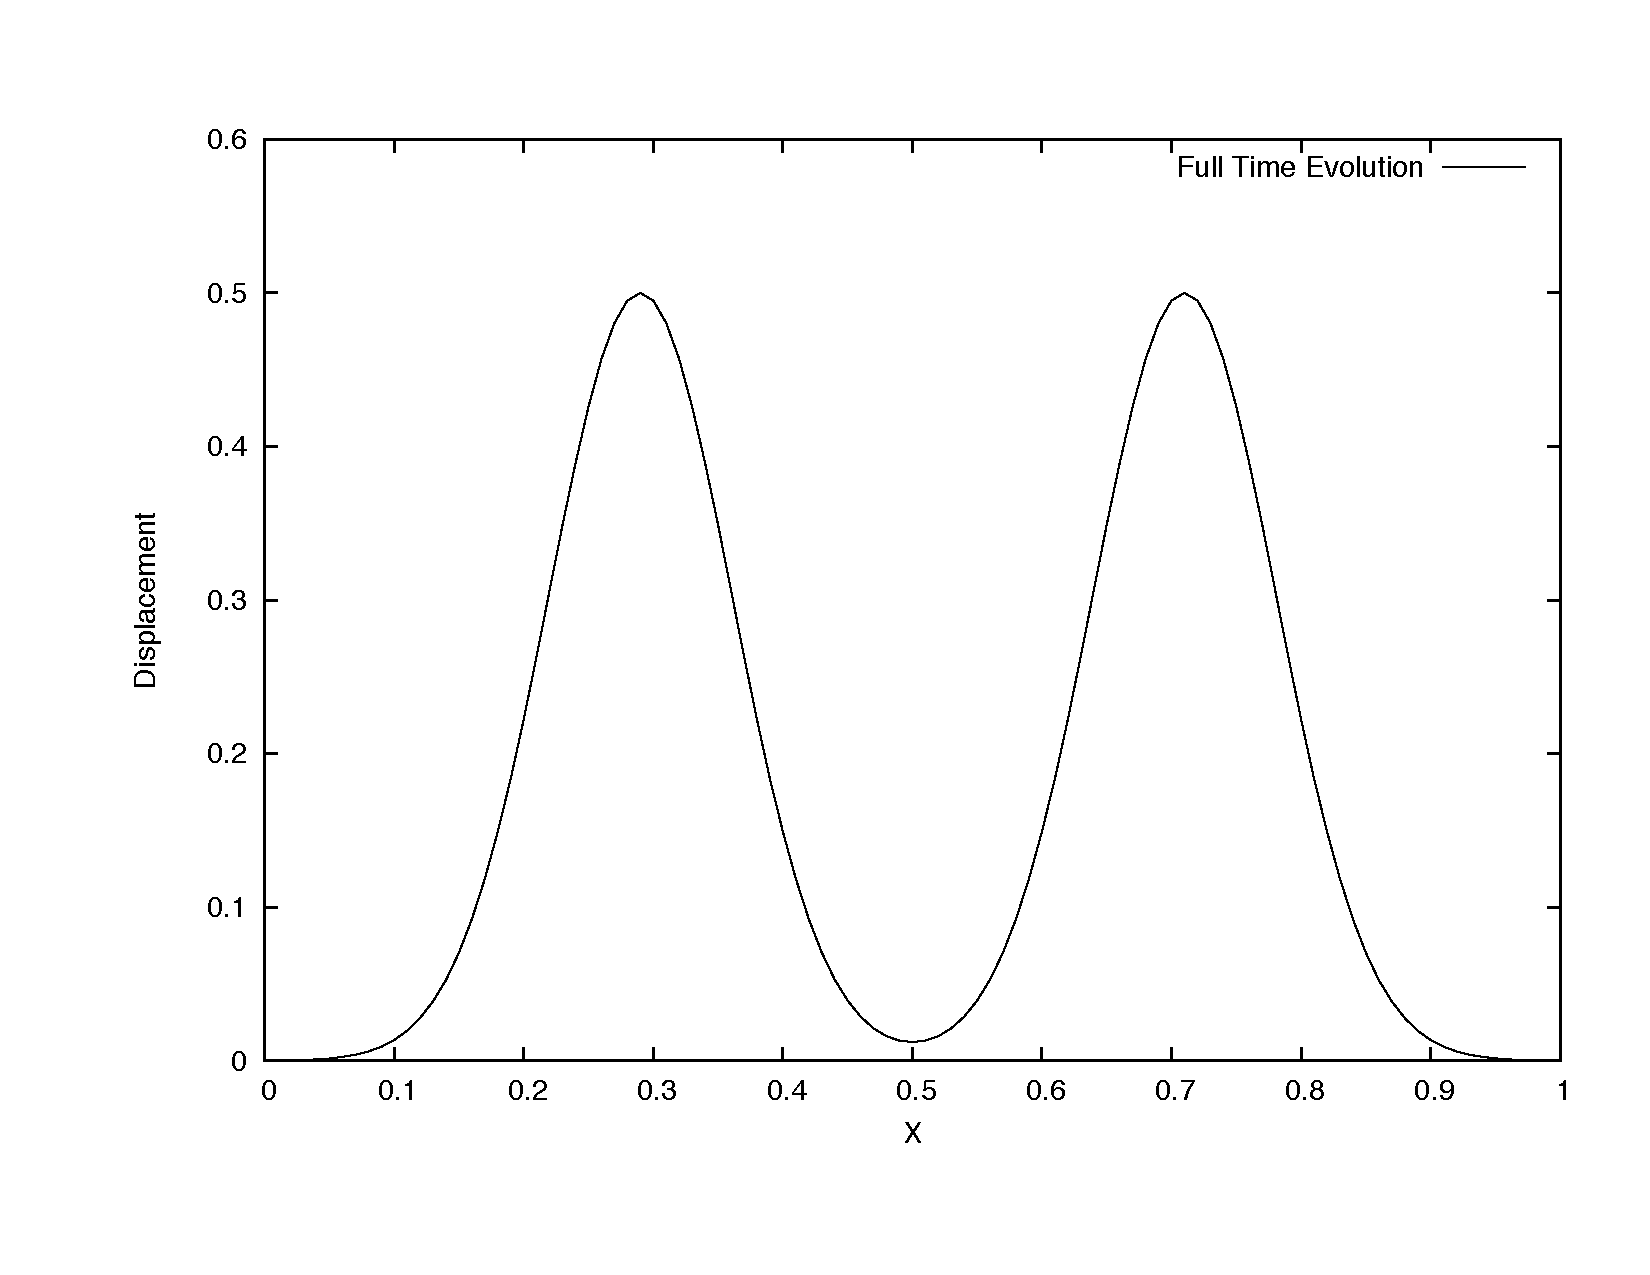
\includegraphics[width =110 mm, height = 60mm]{Ex_7_1_100.pdf}
\caption{Final state of the 'bumped' piano wire.}
\label{fig:7_1_100}
\end{figure}

This time evolution shows the clear decay of the initial state into two outward traveling Gaussian wave packets.  The same calculations were repeated using $dt=1e-2$ in order to demonstrate the unstable solution of this system.  This is shown in Figure \ref{fig:7_2}.
\begin{figure}[!h]
\centering
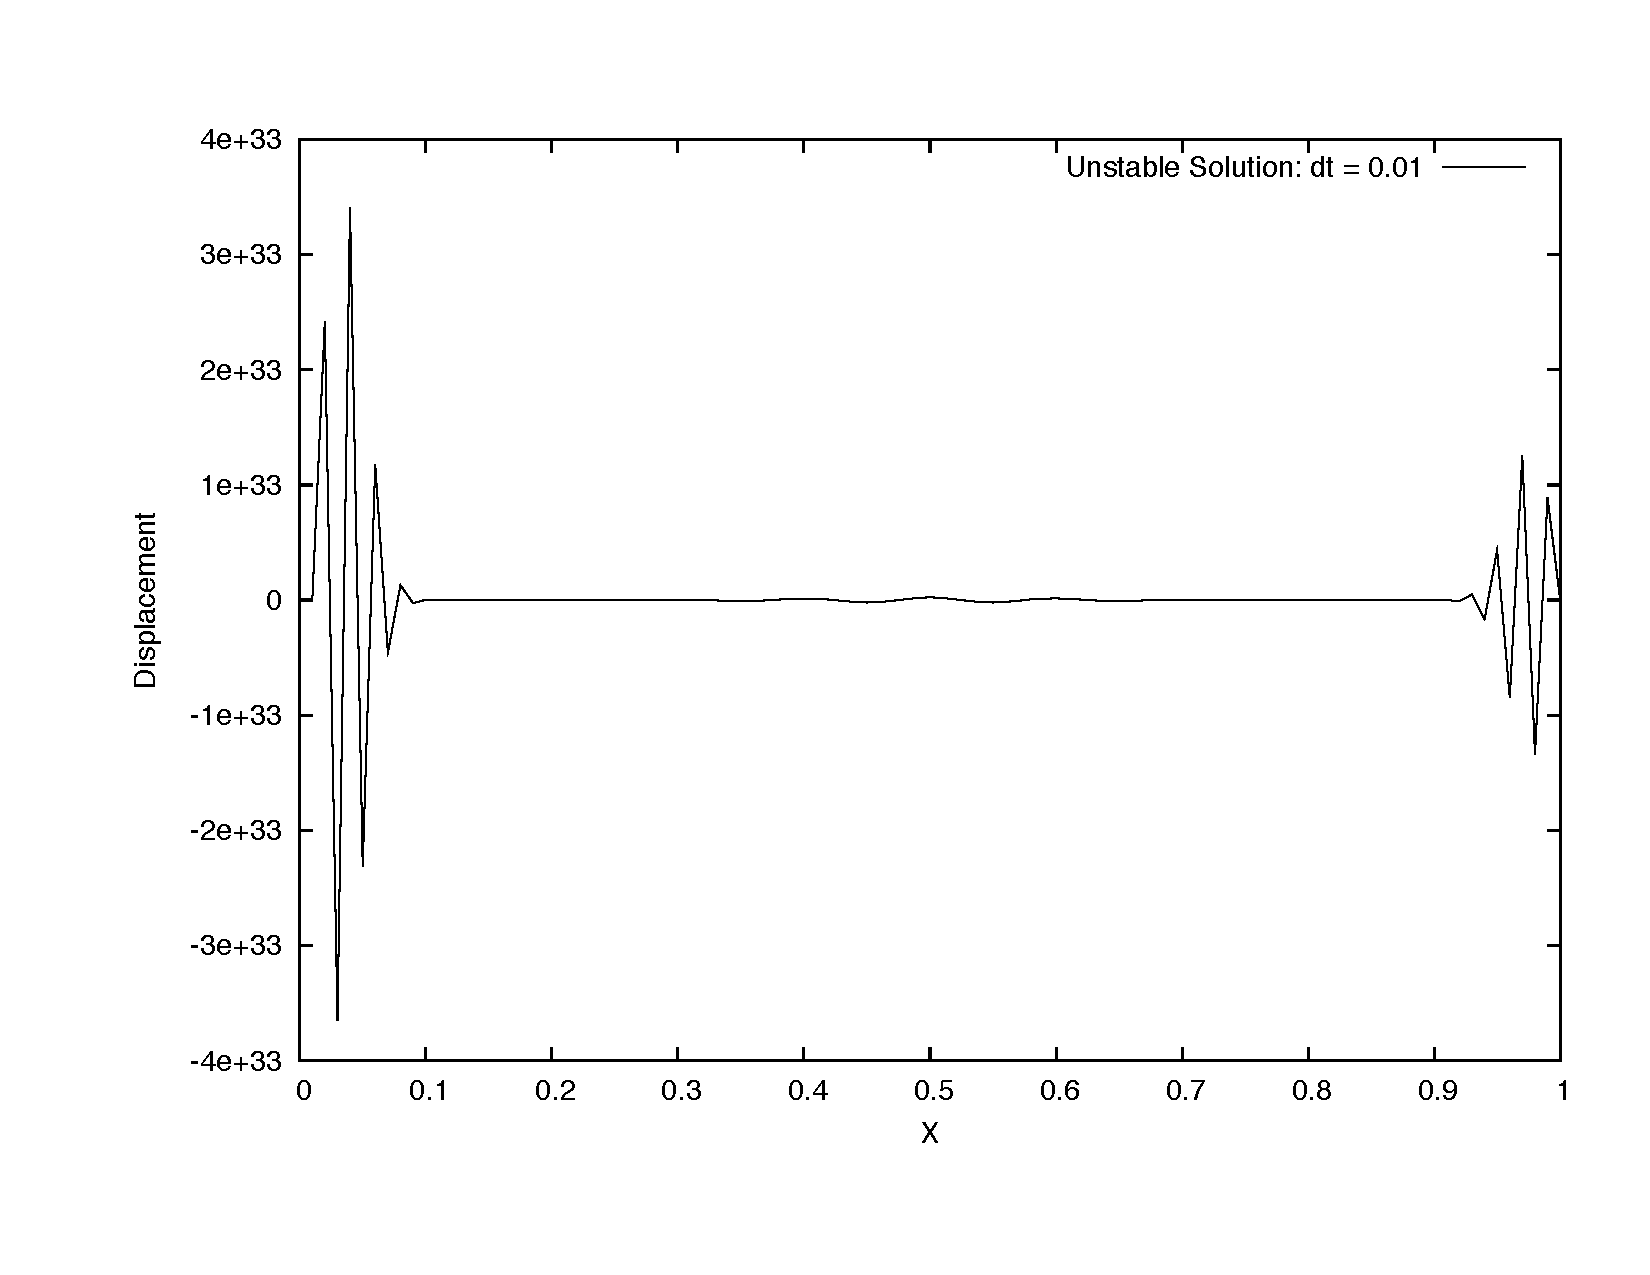
\includegraphics[width =110 mm, height = 60mm]{Ex_7_2.pdf}
\caption{Unstabel solution using the finite difference method.}
\label{fig:7_2}
\end{figure}

Finally, the same system was studied, but now an initial velocity was imposed on the system
\begin{equation}
\label{gaussVel}
\frac{du(x,0)}{dt}=-200c(x-0.5) e^{-100(x+ct-0.5)^2} , 0<x<1
\end{equation}
The series of Figures \ref{fig:7_3_0} through \ref{fig:7_3_100} shows the time evolution of the system with this new condition.
\begin{figure}[!h]
\centering
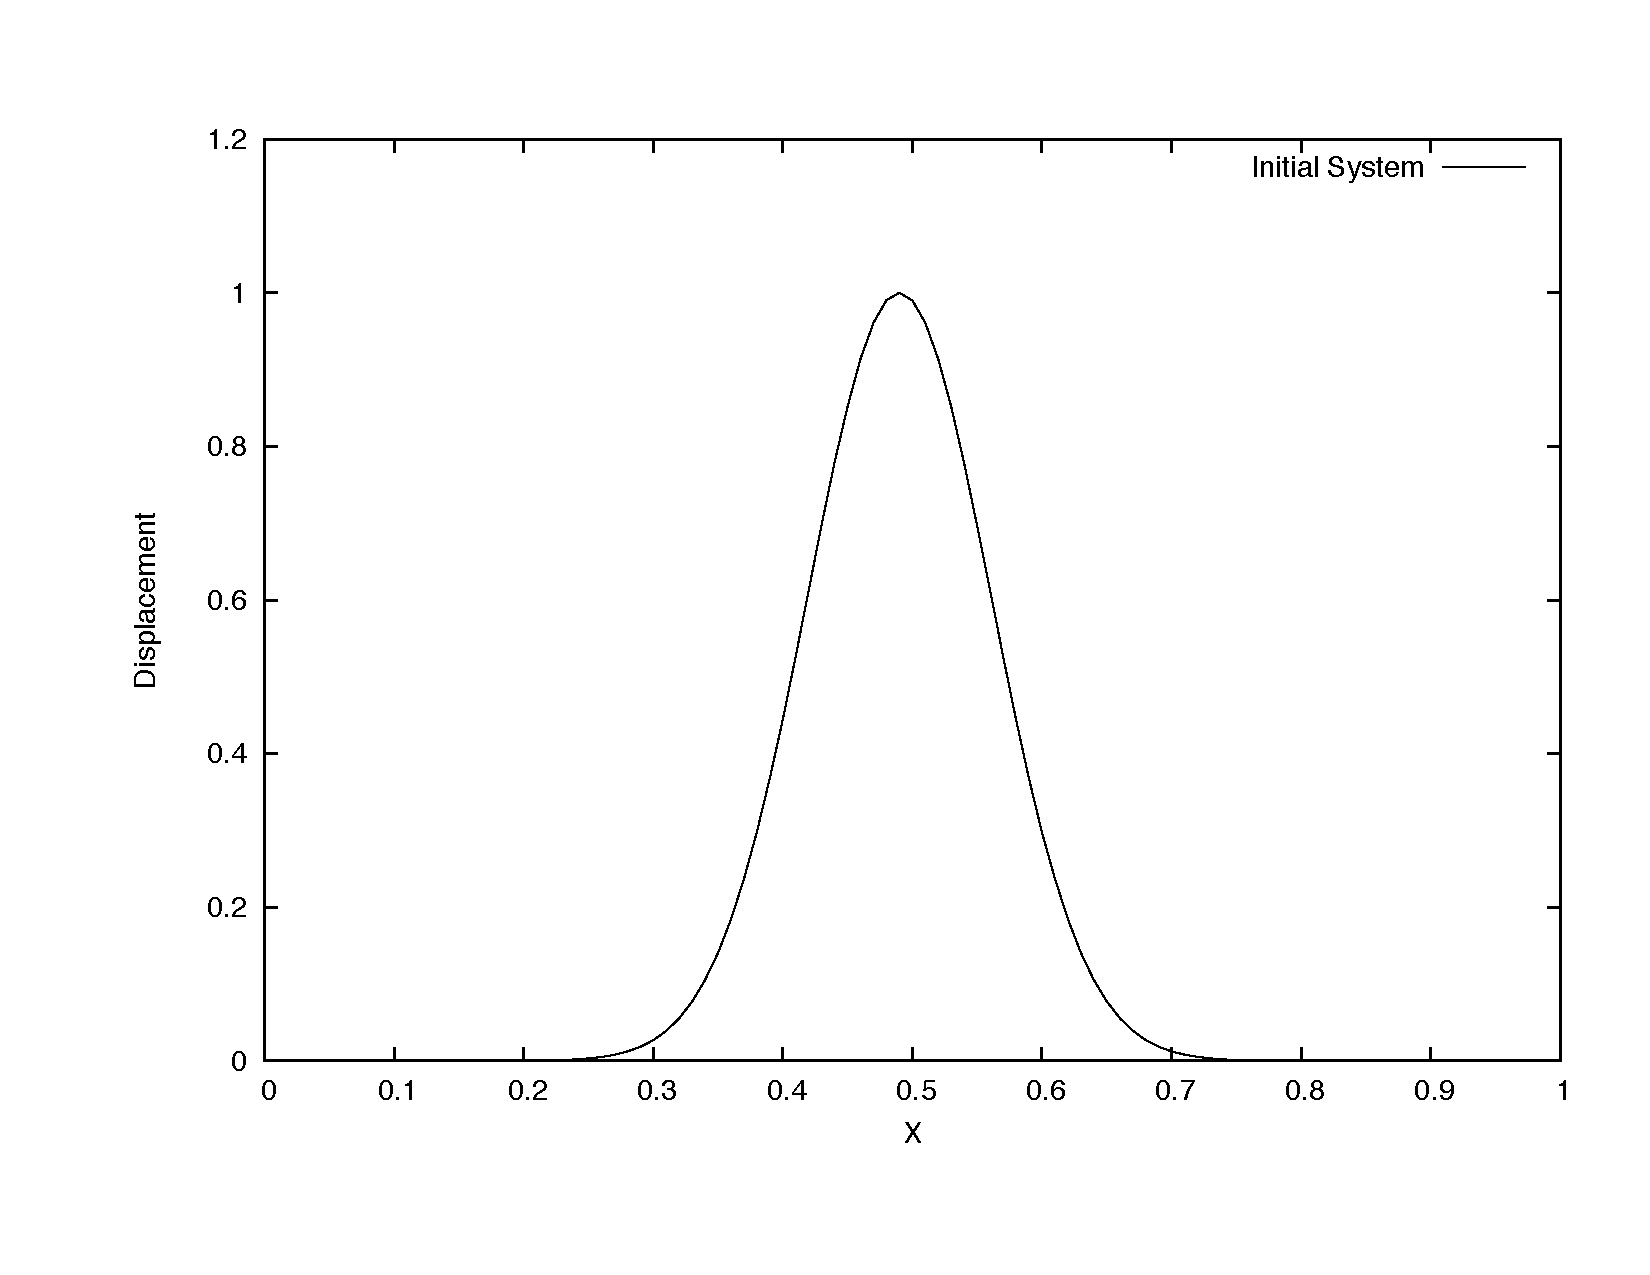
\includegraphics[width =110 mm, height = 60mm]{Ex_7_3_0.pdf}
\caption{Initial state of the 'bumped' piano wire with initial velocity.}
\label{fig:7_3_0}
\end{figure}
\begin{figure}[!h]
\centering
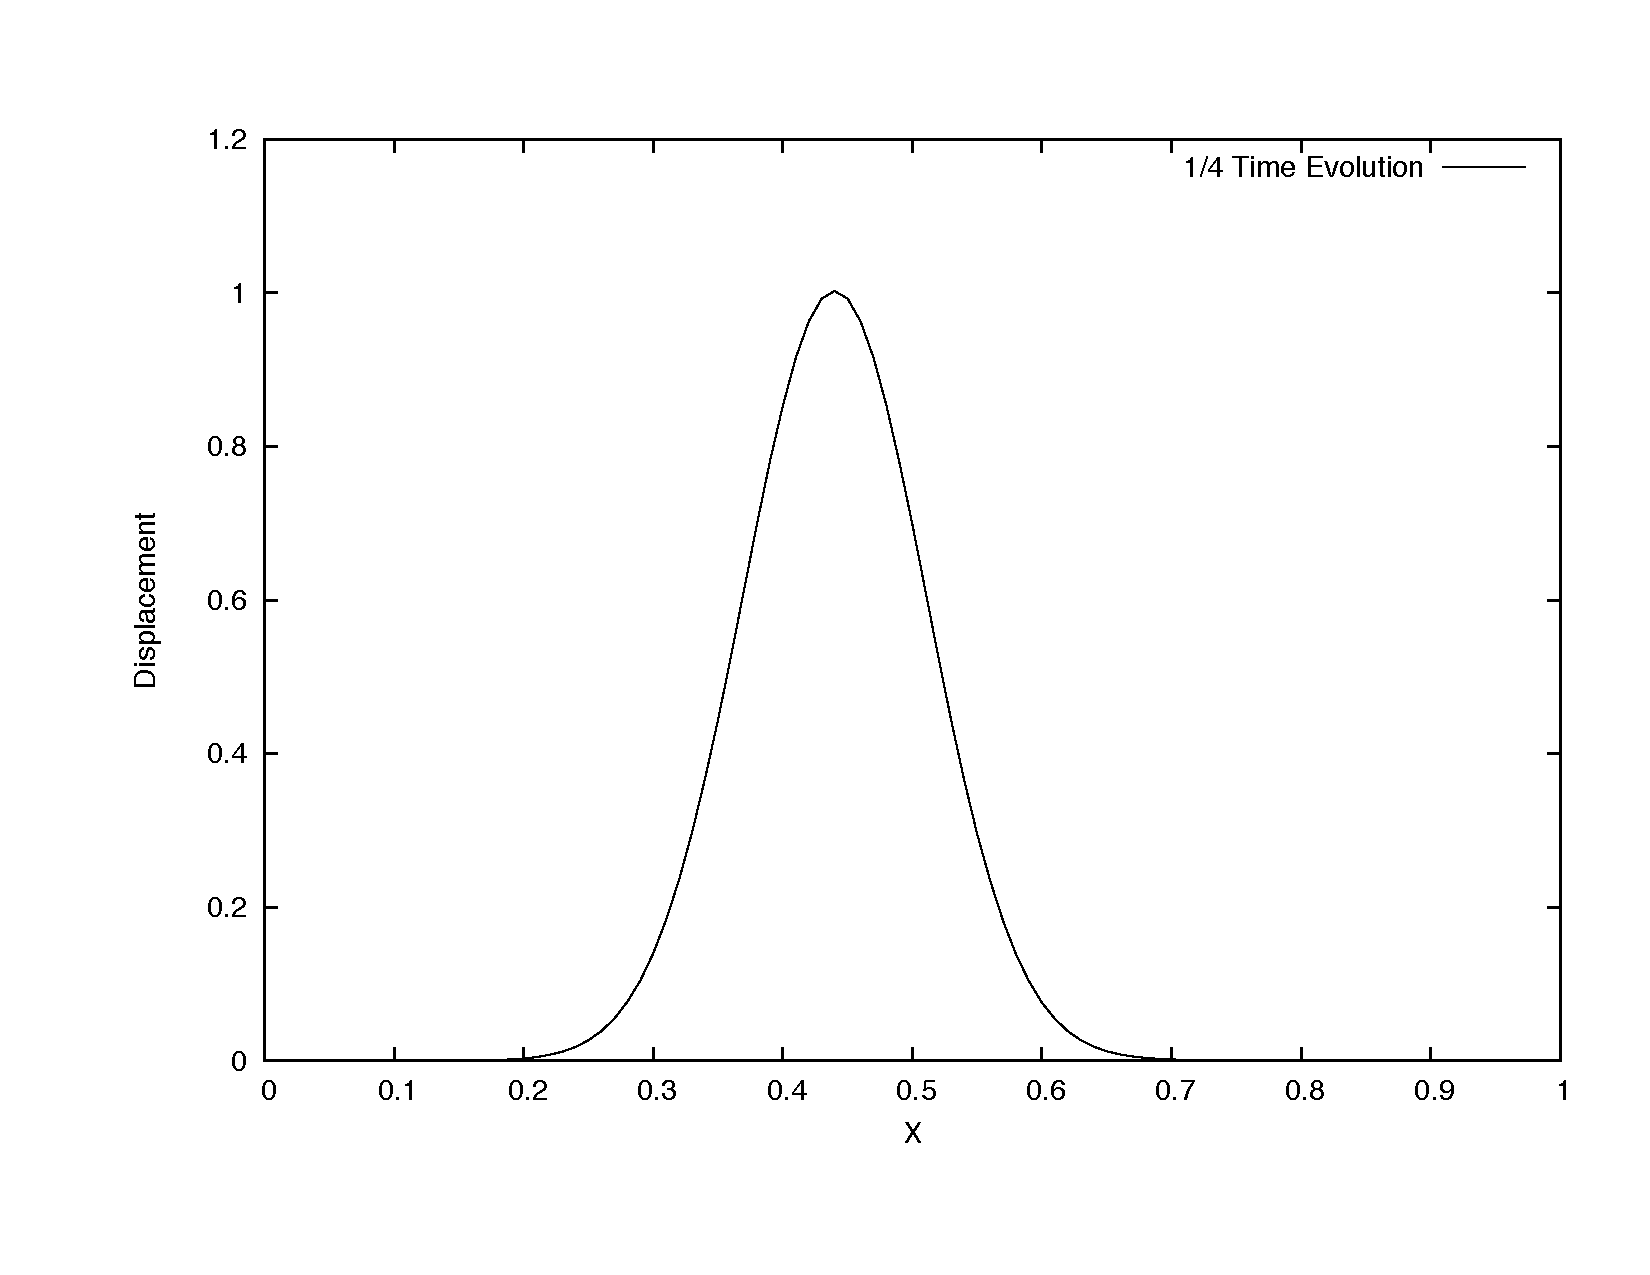
\includegraphics[width =110 mm, height = 60mm]{Ex_7_3_25.pdf}
\caption{'Bumped' piano wire after 1/4 time evolution with initial velocity.}
\label{fig:7_3_25}
\end{figure}
\begin{figure}[!h]
\centering
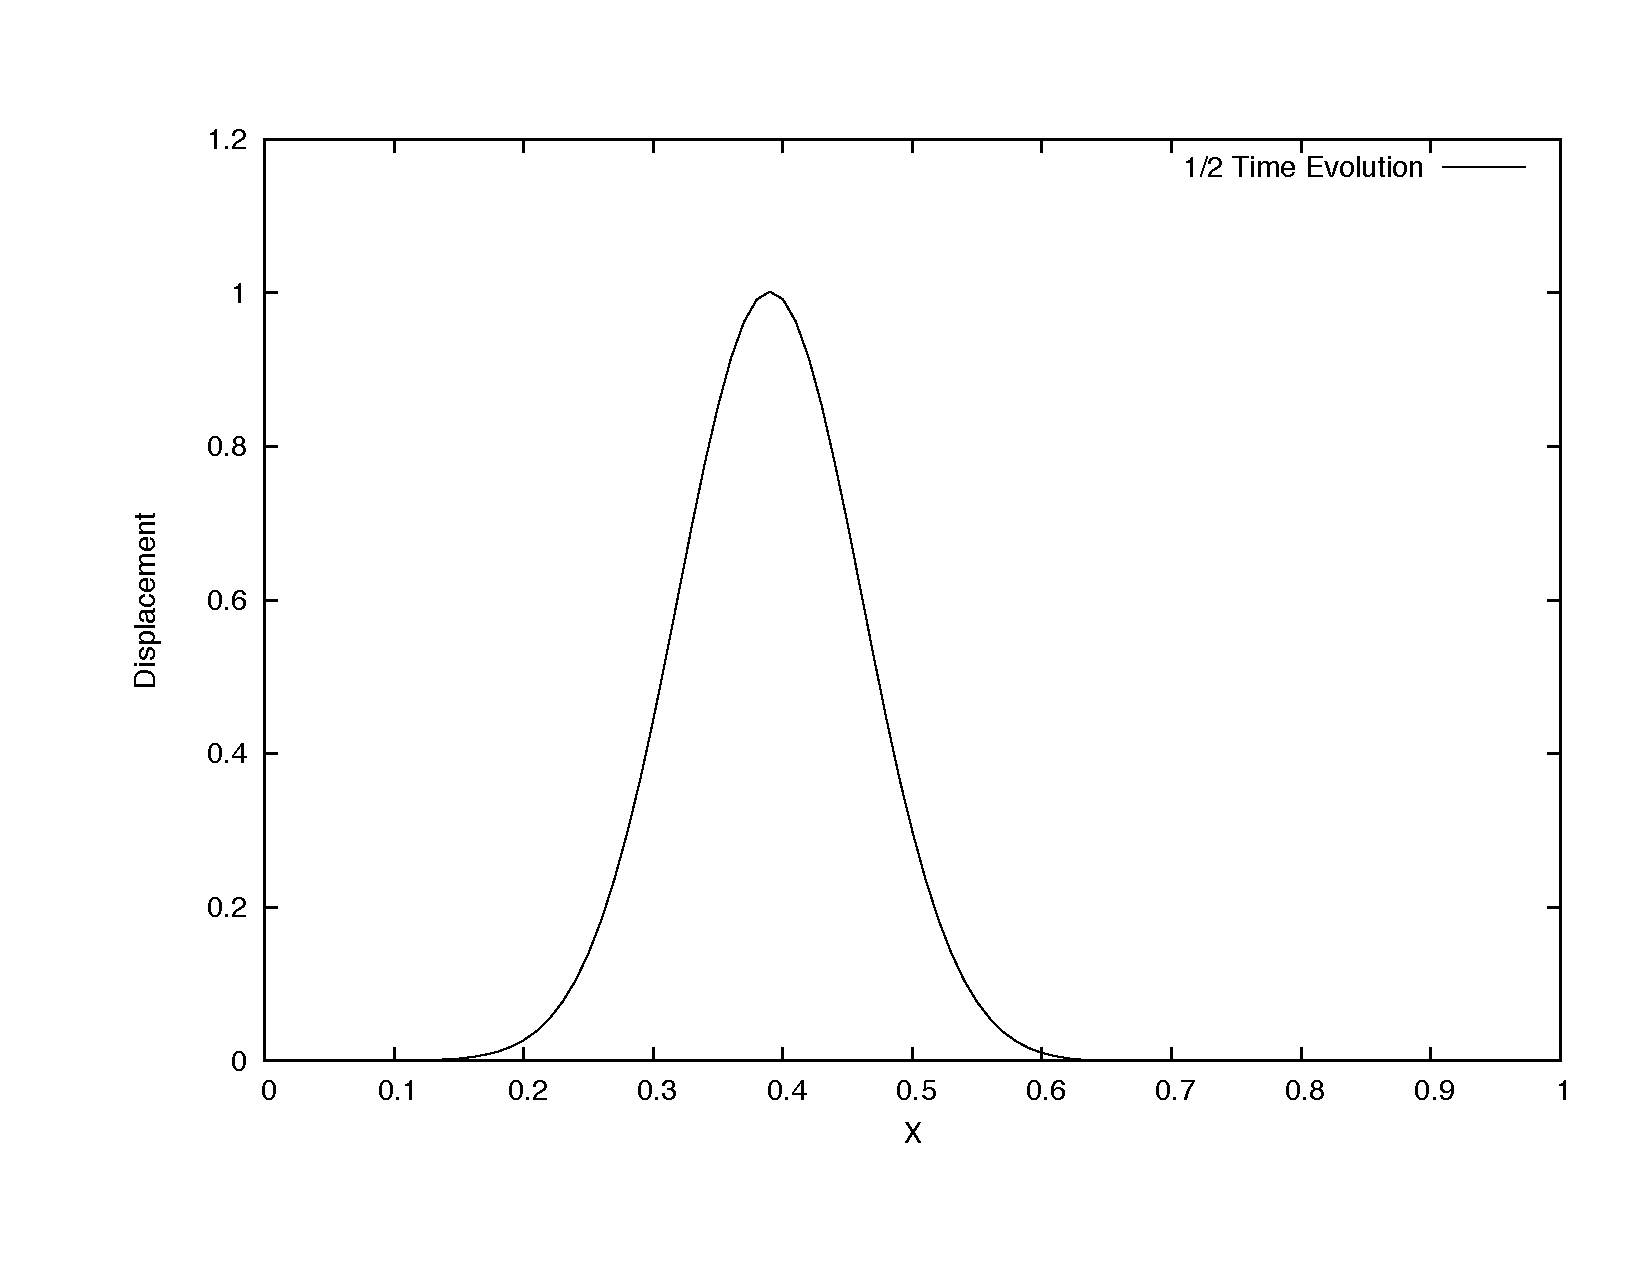
\includegraphics[width =110 mm, height = 60mm]{Ex_7_3_50.pdf}
\caption{'Bumped' piano wire after 1/2 time evolution with initial velocity.}
\label{fig:7_3_50}
\end{figure}
\begin{figure}[!h]
\centering
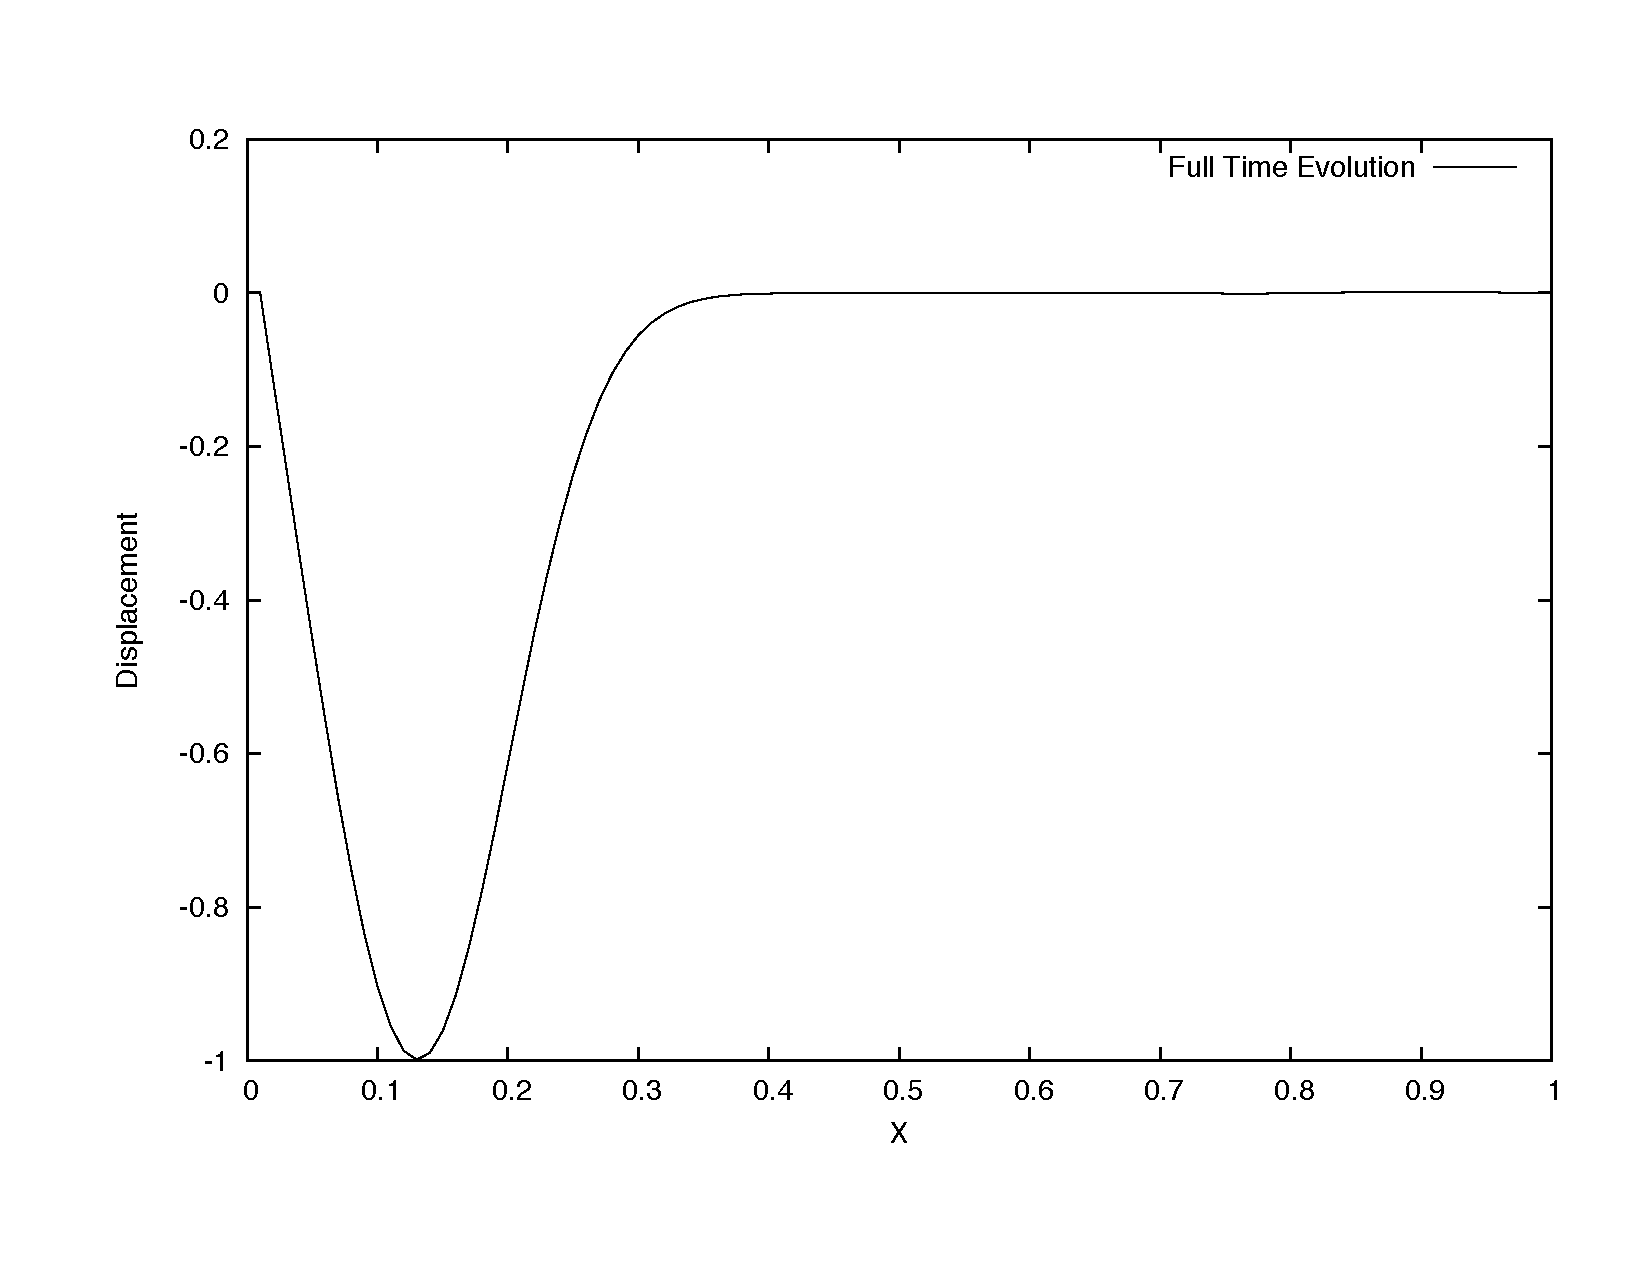
\includegraphics[width =110 mm, height = 50mm]{Ex_7_3_100.pdf}
\caption{Final state of the 'bumped' piano wire with initial velocity.}
\label{fig:7_3_100}
\end{figure}
This new system displays the logical behavior.  The wave packet begins at its initial position in the center of the wire and moves left.  After reaching the fixed endpoint, the wave is reflected back towards the center of the wire with its amplitude in the opposite direction.
\pagebreak
\subsection{Steady State Heat Equation}
The final application of the finite difference technique is the steady state equation.  This equation describes the conduction of heat through a material.  
\begin{equation}
\label{heat}
\nabla^2u(x,y,z,t)= \frac{1}{c^2}\frac{\partial u(x,y,z,t)}{\partial t}, c^2 = \frac{K}{\sigma \rho}
\end{equation}
where $K$ is the thermal conductivity, $\sigma$ is the specific heat, $\rho$ is the density, and $u(x,y,z,t)$ is the temperature.  Considering a thin plate, this equation reduces to a two diminutional Laplace equation.  For this application, the bottom and left edges of the plate were fixed at $100^\circ$ C and the right and top edges at $0^\circ$ C.
\begin{figure}[!h]
\centering
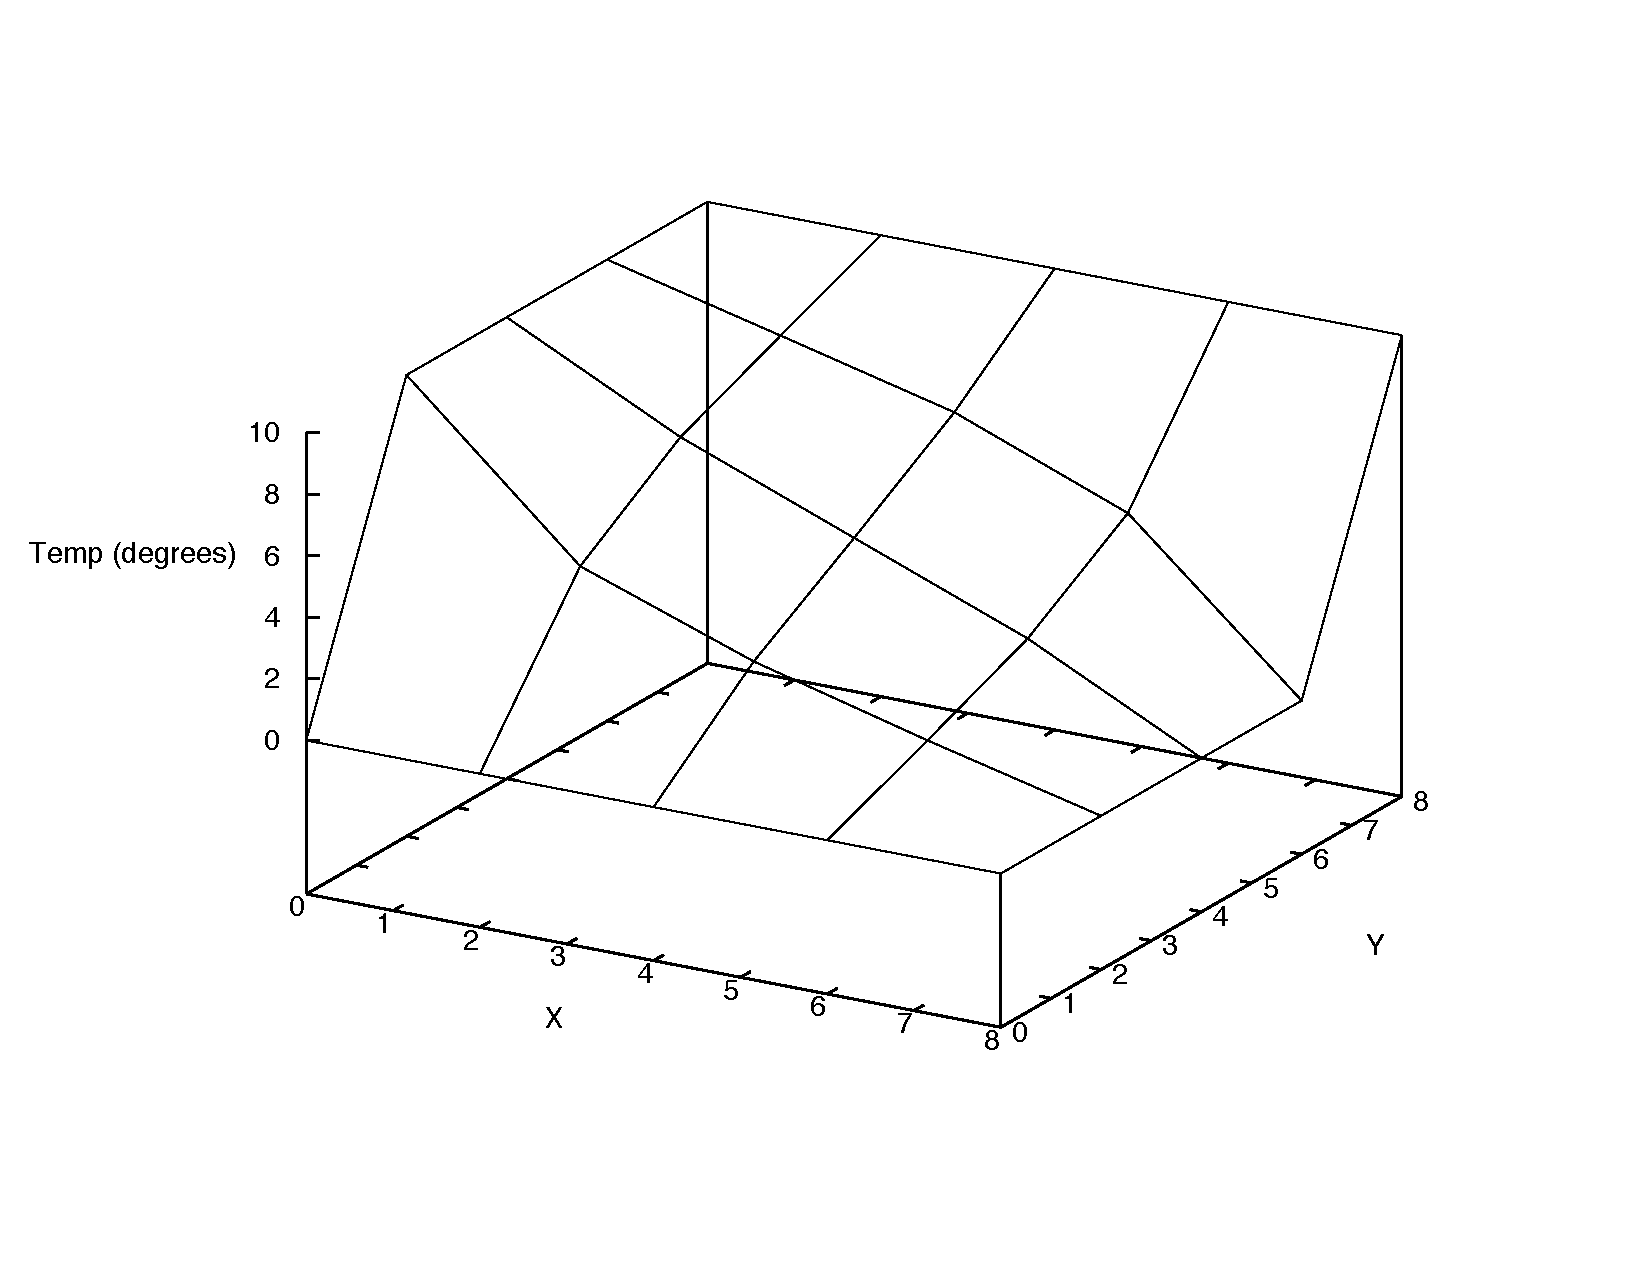
\includegraphics[width =110 mm, height = 70mm]{Ex_7_8.pdf}
\caption{Temperature distribution of a thin sheet.}
\label{fig:7_8}
\end{figure}

Unfortunately, due to the plotting technique, Figure \ref{fig:7_8} appears to have broken the boundary conditions imposed, however in reality the data does not.  This data matches what one would expect to observe:  the heat has dissipated from the hot edges to the cold edges in an exponential decay, as described by the heat equation.




\end{document}

